\documentclass[12pt]{article}

\usepackage[table, svgnames, dvipsnames, xcdraw]{xcolor}
\usepackage{makecell, cellspace, caption}
\usepackage{hyperref}
\usepackage{graphicx}
\usepackage{float}
\usepackage{enumitem}
\usepackage{pifont}
\usepackage{float}
\usepackage{fontawesome5}
\usepackage{longtable}
\usepackage{tabularx}
\usepackage[stable]{footmisc}
\usepackage[a4paper,
		bindingoffset=0in,
		left=0.8in,
		right=0.8in,
		top=0.8in,
		bottom=1.5in,
		footskip=.5in]{geometry}
\usepackage{xepersian}

\settextfont{Vazirmatn}
\setlatintextfont{Arial}
\linespread{1.25}

\author{متین اعظمی}
\author{محمد حسینی}
\author{عسل خائف}
\author{ارشیا شفیعی}
\author{شیدا عابدپور}
\author{امیرعلی لطفی}
\author{زهرا معصومی}
\title{سامانه کارا}

\begin{document}

	\begin{figure}
		\centering
		
\includegraphics[width=0.3\textwidth]{files/logo}
	\end{figure}
	\begin{center}
		دانشگاه اصفهان\\
		دانشکده مهندسی کامپیوتر
		\vspace{2\baselineskip}

		{\Huge \textbf{سامانه کارا}}\\

		\vspace{1\baselineskip}
		کاریابی هدفمند در سازمان‌ها، شرکت‌ها و صنایع\\

		\vspace{2\baselineskip}
		\textbf{پدیدآورندگان به ترتیب الفبا:}\\
		متین اعظمی\\
		محمد حسینی\\
		عسل خائف\\
		ارشیا شفیعی\\
		شیدا عابدپور\\
		امیرعلی لطفی\\
		زهرا معصومی\\
		\vspace{2\baselineskip}
		\textbf{«گروه 3»}\\
		\vspace{3\baselineskip}
		{\textbf{استاد راهنما:}}
		دکتر محمدرضا شعرباف\\
		\vspace{3\baselineskip}
		ترم پاییز 1401

	\end{center}

	\newpage
	\tableofcontents
	\newpage
	\listoftables
	\newpage
	\listoffigures
	\newpage

	\section{سند تبیین نیازمندی‌ها}

	\subsection{مقدمه}
	در این بخش به تبیین نیازمندی‌های سیستم می‌پردازیم که در قالب استاندارد 1998-830
	\textbf{\lr{\textbf{\hyperref[ref:std]{Std}} \textbf{\hyperref[ref:ieee]{IEEE}}}}
	بیان شده است.
	با توجه به افزایش روزافزون مسئله کاریابی، نیاز به بستری برای تسهیل و تسریع این فرایند حس می‌شود. بدیهی است که مدیریت این فرایند و اطمینان یافتن از درست طی شدن آن نیاز به برنامه‌ریزی دقیقی دارد.
	در این پروژه سامانه‌ای طراحی شده است که علاوه بر کمک به کارجویان جهت کاریابی آسان‌تر و جلوگیری از مراجعه حضوری به دفاتر کاریابی و استفاده از روش‌های سنتی، کمک به کارفرمایان جهت استخدام دقیق و بهتر کارجویان خود را در نظر داشته باشد.


	\subsubsection{هدف}
	سند تبیین نیازمندی‌های نرم‌افزار و یا به اختصار
	\textbf{\hyperref[ref:srs]{SRS}}،
	سندی است که در آن به شرح کامل جزئیات نیازمندی‌های سیستم، طریقه ارتباط آنها با سیستم و یا با یکدیگر، عوامل تاثیرگذار بر سیستم، واسط‌های گوناگونی که در بخش‌های مختلف سیستم به کار رفته است و کارکرد محصول از جنبه‌های مختلف می‌پردازد.
	به طور خلاصه، این سند دیدی جامع از محصول را به نمایش می‌گذارد و به سه گروه از افراد کمک می‌کند و نیازمندی‌های آن‌ها به دست آمده است:

	\begin{enumerate}
		\item
		\textbf{کارجویان:}
		این سند نشان‌ دهنده آن است که کارجو از سیستم چه انتظاراتی دارد و چه نیازمندی‌هایی باید برای این انتظارات در نظر گرفته شود. این کار باعث شده کارجو درک بهتری از نیازهای خود پیدا کرده و نیازهایش را مدیریت کند.
		\item
		\textbf{کارفرمایان:}
		این سند نشان دهنده آن است که کارفرما از سیستم چه انتظاراتی دارد و جهت تسهیل و تسریع روند استخدام چه نیازمندی‌هایی باید برای او در نظر گرفته شود. این کار باعث شده کارفرما درک بهتری از نیاز‌های خود پیدا کرده و آن‌ها را مدیریت کند.
		\item
		\textbf{مدیر سیستم:}
		این دسته از افراد نیز همانند کارجویان و کارفرمایان، باید دید کلی و جامعی از نیازمندی‌های سیستم داشته باشند. لذا این سند یک توافق اولیه میان کارجو و کارفرما و مدیر سیستم برای آنچه سیستم باید انجام دهد، به وجود می‌آورد و حلال مشکلات بسیاری خواهد بود.
	\end{enumerate}
	همچنین در آغاز پروژه به کمک این سند می‌توان پیش‌بینی اولیه‌ای از وضعیت زمان‌بندی و هزینه‌های پروژه انجام داد.

	\subsubsection{قلمرو}
	این پروژه یک سیستم نرم‌افزاری است که به هدف سرعت بخشیدن و بهبود فرایند کاریابی برنامه‌ریزی شده است.
	این سامانه، تحت عنوان "\textbf{کارا}" جهت ثبت آگهی، معرفی شرکت‌های مطرح، انجام آزمون‌های شخصیتی، ساخت رزومه مناسب، تخمین حقوق، ایجاد بستر ارتباط مجازی برای ایجاد پلی بین کارجو و کارفرما و هر قابلیتی که از نظر گروه به بهبود روند کاریابی به کارجو و کارفرما کمک می‌کند، طراحی شده است.
	انتظار می‌رود که این سامانه بتواند با دریافت مشخصات معتبر و احراز هویت، در فضایی امن، امکان استفاده کاربران از امکانات تارنما را به آن‌ها بدهد و در حیطه استخدام و کاریابی به کارفرمایان و کارجویان کمک شایانی کند.
	در این سامانه تا آنجایی که امکان داشته طراحی به صورتی انجام شده که عوام جامعه هم بتوانند با آن کار کنند، همچنین سعی شده تا محدودیت‌های افراد با شرایط خاص نیز در نظر گرفته شود. با این حال سامانه امکان بهبود و توسعه جهت بهتر شدن را دارد ولی به دلیل محدودیت زمانی موجود به بخش‌های اشاره شده در فوق بسنده کرده‌ایم.

	\subsubsection{تعاریف، سرنام‌ها و کوته‌نوشت‌ها}
	\begin{itemize}
		\item
		\textbf{SRS\label{ref:srs}}
		کوته‌شده عبارت
		\lr{Specification Requirement Software}
		است.
		\item
		\textbf{IEEE\label{ref:ieee}}
		کوته‌شده عبارت
		\lr{Institute of Electrical and Electronics Engineers}
		است.
		\item
		\textbf{STD\label{ref:std}}
		کوته‌شده واژه
		\lr{Standard}
		است.
		\item
		\textbf{HTTPS\label{ref:https}}
		کوته‌شده عبارت
		\lr{Hyper Text Transfer Protocol Secure}
		است که یک پروتکل ارتباطی برای انتقال امن اطلاعات در شبکه‌های کامپیوتری است که به صورت خاص در اینترنت استفاده می‌شود.
		\item
		\textbf{SSL\label{ref:ssl}}
		کوتاه‌شده عبارت
		\lr{Secure Socket Layer}
		است که پروتکلی است برای ردّ و بدل کردن سندهای خصوصی از طریق اینترنت.
		\item
		\textbf{HTML\label{ref:html}}
		یک زبان نشانه‌گذاری است که کوته‌شده واژه
		\lr{HyperText Markup Language}
		است.
		\item
		\textbf{CSS\label{ref:css}}
		کوتاه شده عبارت
		\lr{Cascading Style Sheets}
		است.
		\item
		\textbf{جاوا اسکریپت:\label{ref:js}}
		\lr{JavaScript}
		(به اختصار \lr{JS})
		یک زبان برنامه نویسی است که برای توسعه نرم‌افزارهای مرتبط با وب استفاده می‌شود.
		\item
		\textbf{مرورگر وب:\label{ref:browser}}
		نوعی نرم‌افزار کاربردی است که برای دریافت، نمایش، مرور و ارسال اطلاعات، جستجوی تارنماها در وب جهانی یا یک تارنمای محلی مورد استفاده قرار می‌گیرد.
		\item
		\textbf{پروتکل:\label{ref:protocol}}
		به معنی مجموعه‌ای از قوانین و رویه‌ها برای برقراری ارتباط است.
		\item
		\textbf{سیستم عامل:}
		نرم‌افزار سیستمی‌ای است که مدیریت منابع رایانه را به عهده گرفته و بستری را فراهم می‌سازد که نرم‌افزار کاربردی اجرا شده و از خدمات آن استفاده کنند.
		\item
		\textbf{سرور ابری:\label{ref:cs}}
		یک نوع سرور می‌باشد که در رایانش ابری ایجاد شده و بر روی بستر اینترنت برای بسیاری از کاربران ارائه می‌شود.
		\item
		\textbf{\lr{Web Server}\label{ref:ws}}:
		نرم‌افزاری کامپیوتری است که اصلی‌ترین وظیفه آن ارائه اطلاعات و سرویس‌های درخواست شده در قالب صفحات وب به کاربران است.
		\item
		\textbf{PDF\label{ref:pdf}}:
		کوته‌شده عبارت
		\lr{Portable Document Format}
		است.
		\item
		\textbf{JPG/JPEG\label{ref:jpg}}
		کوته‌شده عبارت
		\lr{Joint Photographic Expert Group}
		است.
		\item
		\textbf{SSD\label{ref:ssd}}
		کوته‌شده‌ عبارت
		\lr{Solid-State Drive}
		است.
		\item
		\textbf{Captcha\label{ref:captcha}}
		کوته‌شده عبارت
		\lr{Completely Automated Public Turing test to tell Computers and Humans Apart}
		می‌باشد.
		\item
		\textbf{رمزنگاری:\label{ref:enc}}
		ابزاری است که برای انتقال و نگه‌داری امن اطلاعات استفاده می‌شود. در واقع هدف رمزنگاری این است که داده را به گونه‌ای نگه‌داری یا ارسال کند که فقط کسانی که مجاز هستند، به اصل داده‌ها دسترسی داشته باشند.
		\item
		\textbf{یادگیری ماشین:\label{ref:ml}}
		معادل آن
		\lr{Machine Learning}
		است که مطالعه‌ی الگوریتم‌ها و مدل‌های آماری مورد استفاده‌ی سیستم‌های کامپیوتری است که به‌جای استفاده از دستورالعمل‌های واضح، از الگوها و استنباط برای انجام وظایف استفاده می‌کنند.
		\item
		\textbf{رابط کاربری گرافیکی:\label{ref:gui}}
		یک محیط گرافیکی که نرم‌افزارهای رایانه، برای راهنمایی و کاربری بهتر انسان بکار می‌گیرند.
		\item
		\textbf{طراحی واکنش‌گرا:‌\label{ref:responsive}}
		رابط کاربری گرافیکی‌ای که با تغییر اندازه صفحات، نوع چیدمان عناصر در صفحه را تغییر دهد.
		\item
		\textbf{کاربر‌پسند:}
		ویژگی نرم‌‏افزار یا سخت‏‌افزاری که کار کردن با آن و یادگیری استفاده از آن، برای کاربران تازه‏‌کار یا بی‌‏تجربه، ساده و آسان باشد.
		\item
		\textbf{مودم:}
		یک از ابزار رایانه‌ای است که برای اتصال دو رایانه به یکدیگر و شبکه‌های مختلف از راه خطوط گوناگون مخابراتی استفاده می‌شود.
		\item
		\textbf{کارت شبکه:‌}
		سخت‌افزار رایانه به صورت کارتی در شیارهای توسعه مادربورد رایانه قرار می‌گیرد و رایانه را به شبکه متصل می‌کند.
		\item
		\textbf{پایگاه‌داده:}
		مجموعه‌ای سازمان یافته از داده‌های ذخیره شده و الکترونیکی است.
		\item
		\textbf{سیستم مدیریت پایگاه‌داده:}
		معادل عبارت
		\lr{Database Management System}
		یا به اختصار DBMS است که نرم‌افزاری است که از مجموعه‌ای از ابزارها و بخش‌های مرتبط با هم به منظور فراهم آوردن امکان مدیریت کامل اطلاعات ذخیره شده در پایگاه‌داده تشکیل شده است.
		\item
		\textbf{دستیار صوتی:}
		یک عامل نرم‌افزاری است که با صوت به کاربر کمک می‌کند از سیستم استفاده کند.
		\item
		\textbf{\lr{QR Code}}
		کوته‌شده عبارت
		\lr{Quick-Response Code}
		و معادل فارسی آن "رمزینه پاسخ سریع" می‌باشد که یک رمزینه ماتریسی است که دربردارنده چیدمانی از نقطه‌های مربع‌شکل سیاه‌رنگ (با نام ماژول) بر روی زمینه سفید است. داده نهفته می‌تواند نوشته، نشانی وب، پیامک، شماره تلفن، اطلاعات کارت ویزیت یا داده دیگری باشد.
		\item
		\textbf{تارنوشت:}
		نوعی وبگاه است که حاوی اطلاعاتی مانند: گزارش روزانه، اخبار، یادداشت‌های شخصی یا مقالات علمی مورد نظر طراح آن است. در این سیستم تارنوشت به منظور انتشار نویسه‌های مدیر سیستم ایجاد شده است.
		\item
		\textbf{نویسه‌ تارنوشت:}
		یک نوشته در تارنوشت است. معادل انگلیسی آن
		\lr{Blog Post}
		می‌باشد.
		\item
		\textbf{شخص حقیقی:}
		هر انسانی که زنده است و در جامعه زندگی می‌کند یک شخص حقیقی نامیده می‌شود که این شخص دارای شخصیت و حقوق مخصوص به خود می‌باشد.
		\item
		\textbf{شخص حقوقی:}
		هر سازمان، نهاد، وزارتخانه یا مؤسسه‌ای است که فعالیت تجاری یا غیر‌تجاری خاصی را انجام می‌دهد.
		\item
		\textbf{کارجو:}
		یک شخص حقیقی است که به دنبال استخدام می‌باشد.
		\item
		\textbf{کارفرما:}
		یک شخصیت حقیقی یا شخصیت حقوقی است که به دنبال استخدام کارجو در موقعیت شغلی‌های  می‌باشد.
		\item
		\textbf{شرکت:}
		هر سازمان، نهاد، یا مو‌ٔسسه‌ای که توسط یک کارفرما در سیستم ثبت شده باشد.
		\item
		\textbf{پشتیبان تارنما:}
		شخصی حقیقی که وظیفه کمک و راهنمایی کاربران را به منظور استفاده از سیستم دارد.
		\item
		\textbf{پست الکترونیک معتبر:}
		هر رشته که ساختار درست یک پست الکترونیک را داشته باشد.
		\item
		\textbf{وضعیت روند رزومه:}
		هر رزومه ارسال شده در سیستم، در یکی از وضعیت‌های زیر قرار خواهد داشت:
		\begin{itemize}
			\item
			\textbf{ارسال شده:}
			وضعیت اولیه هر رزومه است که به معنای ارسال موفقیت آمیز رزومه از سمت کارجو به سمت کارفرما می‌باشد.
			\item
			\textbf{‌مشاهده شده توسط کارفرما:}
			رزومه توسط کارفرما دیده شده است؛ ولی هنوز تأیید نشده است.
			\item
			\textbf{در دست بررسی:}
			رزومه در اولویت بررسی سازمان قرار گرفته است و کارشناسان سازمان در حال بررسی بیشتر بر روی رزومه هستند.
			\item
			\textbf{تایید اولیه:}
			مرحله بررسی با موفقیت پشت سر گذاشته شده است و کارفرما رزومه را تایید اولیه کرده است.
			\item
			\textbf{دعوت به مصاحبه:}
			کارفرما پس از تایید اولیه، کارجو را به مصاحبه دعوت کرده است.
			\item
			\textbf{رد شده:}
			رزومه توسط کارفرما به هر دلیل رد شده است.
			\item
			\textbf{منجر به استخدام:}
			کارفرما پس از انجام مصاحبه، کارجو را استخدام کرده است.
			\item
			\textbf{لغو توسط کارجو:}
			کارجو درخواست استخدام خود را لغو کرده است و رزومه دیگر برای کارفرما نمایش داده نمی‌شود.
			\item
			\textbf{منقضی شده:}
			اگر کارفرما پس از گذشت ۴۵ روز از ارسال رزومه،‌ وضعیت نهایی آن را مشخص نکند، رزومه به این وضعیت تغییر می‌کند.
			\item
			\textbf{آگهی بسته شده:}
			اگر آگهی مربوطه بسته شده باشد، رزومه در هر وضعیتی که باشد به این وضعیت تغییر می‌کند.
		\end{itemize}
		\item
		\textbf{آزمونک‌های صحت‌سنجی:}
		آزمونک‌هایی که توسط سیستم به صورت آنلاین برای هر کارجو برگزار می‌شود و صحت تسلط کارجو بر یک مهارت را ارزیابی می‌کند.
		\item
		\textbf{توصیه‌نامه:}
		یک فایل الکترونیکی به فرمت \textbf{\hyperref[ref:pdf]{PDF }} که در آن یک کارجو برای کار در یک موقعیت شغلی توصیه شده است.
		\item
		\textbf{اشتراک ویژه:}
		کاربران سیستم با پرداخت هزینه‌‌‌، اشتراک ویژه سیستم را تهیه می‌کنند که با این اشتراک مجموعه‌ای از قابلیت‌های سیستم برای آن‌ها فعال می‌شود.
		\item
		\textbf{اسناد و اطلاعات محرمانه:}
		این اسناد شامل هر مدرک ارسالی توسط کارجویان و کارفرمایان و اطلاعات وارد شده آن‌ها در سیستم می‌باشد.
		\item
		\textbf{سیستم پیشنهاد دهنده موقعیت‌های شغلی:}
		یک عامل نرم‌افزاری است که با استفاده از داده‌های جمع‌آوری شده از سوی یک کارجو نظیر سوابق جستجو، رزومه، و آگهی‌های نشان شده، موقعیت‌های شغلی جدید مناسب آن کارجو را به دست می‌آورد و به کارجو پیشنهاد می‌دهد.
		\item
		\textbf{تالار گفتگو:}
		یک محیط مجازی است که کاربران سیستم می‌توانند به صورت آنلاین در آن با یکدیگر به گفتگو بپردازند.
		\item
		\textbf{گفتگو سریع با پشتیبان:}
		هر کاربر در سیستم از طریق این ویژگی می‌تواند به صورت آنلاین با پشتیبان سامانه در ارتباط باشد.
		\item
		\textbf{ماشین حساب حقوق:}
		یک عامل نرم‌افزاری است که با پردازش بر روی داده‌های وارد شده از سوی دیگر کاربران، که شامل عنوان شغلی؛ سطح ارشدیت؛ سابقه کاری؛ حقوق دریافتی می‌باشد، می‌تواند با دریافت عنوان شغلی، سطح ارشدیت و سابقه کاری یک کاربر، یک حقوق تخمین زده شده پیشنهادی اعلام کند.
		\item
		\textbf{وزارت صمت:}
		سرواژه "وزارت صنعت، معدن و تجارت".
		\item
		\textbf{نماد شرکت:}
		هر تصویر که نشانگر هویت یک سازمان می‌باشد.
		\item
		\textbf{پیش‌نویس آگهی:}
		یک نسخه منتشر نشده از آگهی شغلی که فقط برای کارفرمای مربوطه قابل مشاهده می‌باشد.
		\item
		\textbf{تور مجازی:‌}
		نمایش فضاهای مختلف به صورت ۳۶۰ درجه و فراگیر به بینندگان بوده و با شبیه‌سازی حضور بازدیدکننده در فضای مربوطه جزئیات متعددی از آن فضا را به تصویر می‌کشد.
		\item
		\textbf{یادگیری عمیق:}
		\lr{Deep Learning}
		بخشی از روش‌های \textbf{\hyperref[ref:ml]{یادگیری ماشین}} است که بر روش‌هایی تمرکز دارد که مبتنی بر شبکه‌های عصبی مصنوعی هستند. یادگیری عمیق به رایانه‌ها می‌آموزد آنچه را که به طور طبیعی برای انسان انجام می‌شود، انجام دهند.
		\item
		\textbf{سیستم‌های توصیه کننده:}
		\lr{Recommender Systems}
		با تحلیل رفتار کاربر خود، اقدام به پیشنهاد مناسب‌ترین اقلام (داده، اطلاعات، کالا و…) می‌نماید.
		\item
		\textbf{خوشه‌بندی:}
		\lr{Clustering}
		گروه‌بندی مجموعه‌ای از اشیاء انجام می‌شود، اینکار به این صورت است که اشیاء در یک گروه (به نام خوشه) در مقایسه با دیگر دسته‌ها (خوشه‌ها) مشابه‌تر هستند.
		\item
		\textbf{تشخیص گفتار:}
		\lr{Speech Recognition}
		به معنای استفاده از رایانه و هوش مصنوعی برای تشخیص کلمات و عبارت موجود در صوت انسان و تبدیل آنها به متن به عنوان خروجی است.
		\item
		\textbf{پردازش زبان‌های طبیعی:}
		\lr{Natural Language Processing}
		عبارت است از استفاده از
		\href{https://fa.wikipedia.org/wiki/%D8%B1%D8%A7%DB%8C%D8%A7%D9%86%D9%87}{رایانه}
		برای پردازش
		\href{https://fa.wikipedia.org/wiki/%D8%B2%D8%A8%D8%A7%D9%86_%DA%AF%D9%81%D8%AA%D8%A7%D8%B1%DB%8C}{زبان گفتاری}
		و
		\href{https://fa.wikipedia.org/wiki/%D8%B2%D8%A8%D8%A7%D9%86_%D9%86%D9%88%D8%B4%D8%AA%D8%A7%D8%B1%DB%8C}{زبان نوشتاری}. بدین معنی که رایانه‌ها را قادر سازیم که گفتار یا نوشتار تولید شده در قالب و ساختار یک زبان طبیعی را تحلیل و درک نموده یا آن را تولید نمایند.
		\item
		\textbf{\lr{Chat GPT}:}
		\lr{Chat GPT}
		به معنای
		\lr{Generative Pre-trained Transformer}
		از مدل‌های زبانی هستند که عموماً بر روی مجموعه بزرگی از داده‌های متنی آموزش داده شده‌اند تا متنی شبیه انسان تولید کنند. آنها با استفاده از چندین بلوک از معماری ترانسفورماتور ساخته شده اند.
	\end{itemize}
	\subsubsection{مراجع}
	\begin{itemize}
		\item
		کونگ، دیوید سی: مهندسی نرم‌افزار شئ‌گرا (یک متدولوژی چابک یکنواخت) جلد اوّل. ترجمه: دکتر بهمن زمانی و دکتر افسانه فاطمی، ۱۳۹۴.
		\item
		\lr{Charles Edeki, International Journal of Computer Science and Mobile Applications, Vol.1 Issue. 3, September- 2013, pg. 13-17.}
		\item
		\lr{\textbf{\hyperref[ref:ieee]{IEEE} \textbf{\hyperref[ref:std]{Std}}} 830-1998 \textbf{\hyperref[ref:ieee]{IEEE}} Recommended Practice for Software Requirements Specifications, In \textbf{\hyperref[ref:ieee]{IEEE}} Xplore Digital Library.\\
			\href{http://ieeexplore.ieee.org/Xplore/guesthome.jsp}{http://ieeexplore.ieee.org/Xplore/guesthome.jsp }}
		\item
		\lr{Software engineering: a practitioner's approach, Pressman, Roger S. Palgrave macmillan, 2005.}

	\end{itemize}

	\subsubsection{طرح کلی}
	نیازمندی‌ها و محدودیت‌ها پس از شناسایی در قالب سند
	\textbf{\hyperref[ref:srs]{SRS}}
	طراحی شده است. در این سند ابتدا به شرح کلی مطالب شامل چشم انداز محصول، کارکرد محصول، مشخصات کاربر، قیود، مفروضات و وابستگی‌ها می‌پردازیم. سپس به بررسی نیازمندی‌هایی از جمله نیازمندی‌های کارکردی و کارایی، قیود طراحی، صفت‌های سیستم نرم‌افزاری و سایر نیازمندی‌ها پرداخته می‌شود.

	\newpage
	\subsection{شرح کلی}
	\textbf{کارا}، سامانه‌ای الکترونیکی و قابل دسترسی بر بستر شبکه است. این سامانه به منظور استفاده برای کارجویان و کارفرمایان، جهت بهبود فرآیند کاریابی و استخدام به صورت الکترونیکی راه اندازی شده است. از اهداف این سامانه می‌توان به کاهش مراجعه اشخاص به دفاتر کاریابی و تسریع و بهبود فرایند استخدام اشاره کرد.

	\subsubsection{چشم‌انداز محصول}
	این سامانه با هدف و چشم‌انداز هوشمند‌سازی و هدفمند کردن کاریابی در سازمان‌ها، شرکت‌ها و صنایع مختلف توسعه داده شده است. هدف این سامانه این است که روند آشنایی \textbf{کارفرما} و \textbf{کارجو} با یکدیگر را تا حد امکان ساده کند و همچنین شبکه‌ای از \textbf{شرکت}‌ها، کارجویان، و کارفرمایان پیاده‌سازی کند تا ارتباط و تعامل بین کاربران را افزایش دهد. از امکانات این سامانه می‌توان به پیشنهاد هوشمندانه کارجویان مناسب، طبق نیاز‌های استخدامی کارفرما و پیشنهاد هدفمندانه موقعیت‌های شغلی مناسب به کارجو طبق اطلاعات شخص اشاره کرد.
	در ادامه واسط‌های مختلف این سامانه را بیان می‌کنیم.
	\begin{enumerate}
		\item
		\textbf{واسط‌های سیستم\footnote{\lr{System Interfaces}}}\\
		در این بخش، ارتباط سیستم اصلی با سیستم‌های خارجی و نحوه تعامل و اشتراک‌گذاری اطلاعات بین این سیستم‌ها بررسی می‌شود.
		\begin{itemize}
			\item
			سامانه جهت احراز هویت افراد ثبت‌نامی، نیازمند دسترسی به پایگاه‌داده ثبت احوال است.
			\item
			سامانه جهت احراز هویت اتباع خارجی ثبت‌نامی، نیازمند دسترسی به پایگاه‌داده اتباع خارجی وزارت امور خارجه است.
			\item
			سامانه جهت تایید و اعتبارسنجی شرکت‌ها و سازمان‌‌های ثبت‌نامی، نیازمند دسترسی به پایگاه‌داده وزارت صنعت، معدن و تجارت است.
			\item
			سامانه جهت تایید پست الکترونیک یا شماره همراه با استفاده از کد تایید، ویرایش و بازیابی رمز‌عبور، ارسال اعلان‌های تارنما و سیستم اطلاع‌رسانی موقعیت‌های شغلی،‌ نیازمند سرویس پیام کوتاه و سرویس پست الکترونیک است.
			\item
			برخی قابلیت‌های سامانه نیازمند پرداخت وجه بوده، لذا سامانه نیازمند دسترسی به درگاه پرداخت اینترنتی است.
			\item
			سامانه جهت احراز هویت مالک شماره همراه نیازمند دسترسی به پایگاه‌داده سازمان تنظیم مقررات و ارتباطات رادیویی دارد.
			\item
			سامانه جهت ورود و ثبت‌نام کاربران با کمک حساب کاربری گوگل و لینکدین نیازمند ارتباط با صفحه ورود به حساب گوگل یا لینکدین است.
		\end{itemize}
		\item
		\textbf{واسط‌های کاربر\footnote{\lr{User Interfaces}}}\\
		در این سامانه کاربران باید بتوانند با توجه به سطح دسترسی خود و با استفاده از اتصال به شبکه اینترنت، از هر دو طریق موبایل و رایانه شخصی، از امکانات سامانه استفاده کنند. همچنین رابط کاربری باید به شیوه‌ای طراحی شود که کار با آن ساده باشد و نیاز به آموزش اضافه‌ای نداشته باشد.

		\item
		\textbf{واسط‌های سخت‌افزاری\footnote{\lr{Hardware Interfaces}}}\\
		این سامانه نیاز به ‌خصوصی به سخت‌افزار‌ها ندارد، با این حال فهرستی از واسط‌های مورد نیاز آمده است.
		\begin{itemize}
			\item
			تجهیزات اولیه اینترنتی برای دسترسی به اینترنت نظیر مودم و کارت شبکه
			\item
			گوشی هوشمند با قابلیت اتصال به اینترنت، رایانه‌های شخصی و یا هر سخت‌افرازی که توانایی اجرای نرم‌افزارهایی نظیر \textbf{\hyperref[ref:browser]{مرورگر }}ها را داشته باشد.
			\item
			جهت احراز هویت، هر کاربر نیازمند حداقل یک تلفن همراه یا رایانه شخصی دارای سیم کارت، به منظور دریافت پیامک و استفاده از امکانات سامانه است.
			\item
			هر دستگاهی با قابلیت شناسایی \lr{QR Code}
			\item
			میکروفون برای ضبط رزومه صوتی یا استفاده از دستیار صوتی
			\item
			سرور (برای مدیریت و پردازش داده‌ها)
		\end{itemize}

		\item
		\label{vaset-nrm}\textbf{واسط‌های نرم‌افزاری\footnote{\lr{Software Interfaces}}}\\
		برای استفاده از سامانه،‌ لازم است کاربرها از \textbf{\hyperref[ref:browser]{مرورگر }}‌هایی نظیر Chrome،Firefox ،Microsoft Edge و یا هر مرورگری که از تکنولوژی‌های \textbf{\hyperref[ref:html]{HTML}}،\textbf{\hyperref[ref:css]{CSS}}  و \textbf{\hyperref[ref:js]{JavaScript}} پشتیبانی می‌کند،‌ استفاده کنند.\\
		با توجه به حجم بالای داده‌ها، از سیستم مدیریت پایگاه‌داده MySQL و MongoDB استفاده می‌شود.\\
		این سامانه
		\textbf{\hyperref[ref:responsive]{طراحی واکنش‌گرا}}
		دارد و قابلیت تغییر حالت مؤلفه‌های رابط کاربری خود را در انواع دستگاه‌های مختلف دارد. برای سیستم‌های پیشنهاد دهنده و دستیار صوتی معلولین و پشتیبان از تکنولوژی‌ها و الگوریتم‌های زیر استفاده می‌شود:
		\begin{itemize}
			\item
			Machine Learning
			\item
			Deep Learning
			\item
			Recommender Systems (Content-based filtering)
			\item
			Clustering
			\item
			Speech recognition
			\item
			Natural language processing
			\item
			Generative pre-trained transformer
		\end{itemize}

		\item
		\textbf{واسط‌های ارتباطی\footnote{\lr{Communication Interfaces}}}\\
		این سامانه از \textbf{\hyperref[ref:protocol]{پروتکل }}‌های امن \textbf{\hyperref[ref:https]{HTTPS}} و \textbf{\hyperref[ref:ssl]{SSL}} برای برقراری ارتباط ایمن با سرور بهره می‌برد تا برای \textbf{\hyperref[ref:browser]{مرورگر }}ها امن تشخیص داده شود. این سامانه از شماره تلفن همراه (از طریق پیامک) و پست الکترونیک ثبت شده در هنگام ثبت‌نام کاربر، برای امور اطلاع‌‌رسانی به کاربران استفاده می کند.\\
		هر کدام از کاربران با توجه به سطح دسترسی، با رابط کاربری خاص خود در سامانه مواجه است.

		\item
		\textbf{واسط‌های حافظه\footnote{\lr{Memory Interfaces}}}\\
		این سیستم جهت پاسخ‌دهی سریع به هر نوع کاربر، باید از یک سیستم حافظه‌ای بسیار سریع بهره ببرد و از ساختمان داده‌های مناسب جهت دسترسی‌های مختلف و نیازهای مختلف کاربران به اطلاعات ذخیره شده استفاده کند.\\
		بدیهی است که این سامانه به حافظه قابل توجه و پردازش سريع اطلاعات نیازمند است؛ که به این جهت از حافظه \textbf{\hyperref[ref:ssd]{SSD}} استفاده خواهیم کرد. با توجه به تخمین‌های انجام شده، به ازای هر ده‌هزار کاربر، ۵۰۰ گیگابایت حافظه مورد نیاز است. لازم به ذکر است که در صورت افزایش تعداد کاربران، حافظه‌ مورد نیاز سیستم به نسبت افزایش خواهد یافت.\\
		برای این سیستم پایگاه‌داده عظیمی در نظر گرفته‌ایم. با توجه به ذخیره تمامی اطلاعات در این پایگاه‌‌داده، می‌توان با استفاده از ابزار‌های مخصوص دسترسی به اطلاعات در پایگاه‌های داده در زمان بسیار کوتاهی به اطلاعات مشخصی از یک کاربر خاص دسترسی پیدا کرد.
		\item
		\textbf{واسط‌های عملیات\footnote{\lr{Operations Interfaces}}}\\
		اطلاعات پایگاه‌داده سامانه به صورت خودکار به وبگاه داده می‌شود و همچنین در آن نوشته می‌شود و عملیات دستی در آن وجود ندارد.\\
		سرورهای سامانه به صورت مجزا هستند و به صورت روزانه در سرورهای دیگر پشتیبان‌گیری می‌شود، همچنین مدارک بارگذاری شده همه کاربران به صورت مادام‌العمر روی سرور‌ها باقی می‌ماند.\\
		برای اجرایی شدن این سیستم، به سرورهای قدرتمند برای پردازش و ذخیره‌سازی داده‌ها نیاز است. ترجیحاً یک سرور، کار پردازش اطلاعات و یک سرور مجزای دیگر در جهت پشتیبان‌گیری و ذخیره داده‌ها استفاده شود.\\
		هر کاربر باید بتواند به تاریخچه رزومه‌ها و استخدام‌های مربوط به خود دسترسی داشته باشد.\\
		تمامی اطلاعات مربوط به احراز هویت، همچنین اطلاعات شخصی افراد \textbf{\hyperref[ref:enc]{رمزنگاری}} شده و در پایگاه‌داده ذخیره خواهند شد.\\
		سیستم پیشنهاد دهنده می‌تواند توسط پیامک و پست الکترونیکی اطلاعات جدیدی برای کاربران ارسال کند.\\
		بازبینی تغییرات کلی سیستم باید چندین بار طی شبانه روز تکرار شود. این تغییرات شامل به‌روزرسانی آگهی‌های ثبت شده، به‌روزرسانی لیست افراد شاغل در هر سازمان، به‌روزرسانی صفحه کاربران و به‌روزرسانی محتوای تارنما در هر روز است.

		\item
		\textbf{نیازمندی‌های سازگاری با محل نصب}\\
		این سامانه روی تمام دستگاه‌هایی که دارای \textbf{\hyperref[ref:browser]{مرورگر }} (در "واسط‌های نرم‌افزاری" اشاره شده است) است، اجرا می‌شود و نیازی به نصب ندارد.\\
		ابزارهایی مانند موبایل، تبلت و دستگاه‌هایی که از سیستم عامل‌های مرسوم همانند Android، iOS وWindows Phone  پشتیبانی می‌کنند، در صورتی که حاوی یک مرورگر برای دسترسی به تارنمای سامانه باشند، می‌توانند از این سامانه استفاده نمایند.\\
		تمامی لپ‌تاپ‌ها، رایانه‎‌های شخصی و هر دستگاهی که با استفاده از سیستم عامل‌های Windows،Linux  یا Mac به نحوی دارای یک مرورگر اینترنت باشد، باید بتواند به تارنما دسترسی پیدا کند.
	\end{enumerate}

	\subsubsection{کارکرد محصول}
	سیستم در کل شامل ویژگی‌های زیر است:
	\begin{itemize}
		\item
		این سامانه نحوه مشاهده آگهی‌های شغلی و ارسال رزومه برای آن‌ها را آسان‌تر می‌کند.
		\item
		این سامانه ثبت‌نام کارفرمایان و کارجویان را در سیستم آسان‌تر می‌کند.
		\item
		این سامانه اطلاع‌رسانی درباره وضعیت روند درخواست شغلی را آسان‌تر می‌کند.
		\item
		این سامانه امکان پیشنهاد آگهی‌های شغلی متناسب با رزومه و سوابق فرد را به کارجو فراهم می‌کند.
		\item
		این سامانه احراز‌ هویت کاربران و اعتبارسنجی سازمان‌ها را آسان‌تر می‌کند.
		\item
		این سامانه امکان استفاده نابینایان و سایر افراد کم‌توان را از قابلیت‌های آن فراهم‌ می‌کند.
		\item
		این سامانه امکان پیشنهاد هدفمندانه کارجو‌های مناسب را برای آگهی‌های شغلی مرتبط را برای کارفرما فراهم می‌کند.
		\item
		این سامانه امکان ارزیابی و صحت‌سنجی مهارت‌های کارجو را آسان‌تر می‌کند.
		\item
		این سامانه ارتباط مستقیم بین کارفرما هر آگهی شغلی با کارجو را فراهم می‌کند.
		\item
		این سامانه امکان به اشتراک‌گذاری نظرات کارجویان درباره یک کارفرما را در تالار گفتگو فراهم می‌کند.
		\item
		این سامانه امکان ارتباط مستقیم بین کارجویان و کارفرمایان را از طریق پیام خصوصی آسان‌تر می‌کند.
		\item
		این سامانه امکان ساخت رزومه و شخصی‌سازی آن‌ را برای کارجو آسان‌تر می‌کند.
	\end{itemize}

	\subsubsection{مشخصات کاربر}
	سامانه دارای چهار نوع کاربر است، به طوری که کارجو و کارفرما دارای دو وضعیت می‌باشند:
	\begin{itemize}
		\item
		کارجو
		\begin{itemize}
			\item
			کارجوی احراز‌ هویت نشده
			\item
			کارجوی احراز‌ هویت شده
		\end{itemize}
		به طور کلی این نوع کاربران شامل موارد زیر می‌شوند:
		\begin{itemize}
			\item
			عموم مردم
			\item
			دانشجویان
			\item
			افراد نیازمند شغل
			\item
			…
		\end{itemize}
		\item
		کارفرما
		\begin{itemize}
			\item
			کارفرمای احراز‌ هویت نشده
			\item
			کارفرمای احراز‌ هویت شده
		\end{itemize}
		به طور کلی این نوع کاربران شامل موارد زیر می‌شوند:

		\begin{itemize}
			\item
			موسسات و شرکت‌های خصوصی
			\item
			موسسات و شرکت‌های دولتی
			\item
			…
		\end{itemize}
		\item
		مهمان
		\item
		مدیر سیستم
	\end{itemize}

	\subsubsection{قیود و محدودیت‌ها\footnote{\lr{Constraints \& Limitations}}}
	\begin{itemize}
		\item
		سامانه باید مجوز‌های لازم برای ایجاد تارنمای کاریابی را از وزارت کار و امور اجتماعی اخذ کند.
		\item
		سامانه باید اعتماد‌سازی لازم جهت اعتماد کارجویان و کارفرمایان را برای به اشتراک گذاشتن و قرار‌دادن اطلاعات و مدارک خود در سامانه را انجام دهد.
		\item
		با توجه به اینکه اطلاعات شخصی، شغلی و … کارجویان و همچنین مدارک و اطلاعات شرکت‌ها و کارفرما در سیستم ذخیره شده است، سیستم باید از امنیت بالایی برخوردار باشد.
		\item
		سامانه باید در ۲۴ ساعت شبانه‌روز قابل دسترسی باشد.
		\item
		سامانه فقط با استفاده از \textbf{\hyperref[ref:browser]{مرورگر }}‌های معتبر قابل اجرا خواهد‌ بود.
		\item
		با توجه به این که سیستم نیاز به اطلاع‌رسانی در بخش‌های مختلف سیستم دارد، سیستم باید از منابع و زیرساخت‌های مناسب در جهت تسریع پاسخگویی، کارآمدتر شدن و عدم اختلال در آن استفاده کند.
		\item
		با توجه به وجود امکان پیام خصوصی و تالار گفتگو، سیستم باید زیرساخت‌های کارایی و امنیتی مورد‌نیاز برای این فرایند‌ها را آماده کند.
		\item
		با توجه به تکنولوژی‌های به‌روز و متعددی که در بخش‌های مختلف سیستم استفاده شده است، سیستم باید نیروی انسانی متخصص لازم جهت به‌روزرسانی، پشتیبانی و اشکال‌زدایی را فراهم کند.
		\item
		این سامانه به دلیل گستردگی زیاد و وجود تیم‌های مختلف برای بخش‌های مختلف نیازمند استفاده از فرایند‌ها و متدولوژی‌های چابک است.
		\item
		سامانه باید مجوزهای لازم برای ایجاد تالار‌های گفتگو و پیام‌های خصوصی را از وزارت فرهنگ و ارشاد، وزارت ارتباطات و … کسب کند.
		\item
		سامانه باید فضای تالار‌های گفتگو و پیام‌های خصوصی را طبق قوانین فضای مجازی و مصادیق محتوای مجرمانه کنترل کند.
		\item
		با توجه به گستردگی سامانه، نیاز است که با مشتری در رابطه با بودجه و زمان تحویل پروژه به توافق رسید.
	\end{itemize}

	\subsubsection{مفروضات و وابستگی‌ها\footnote{\lr{Assumptions \& Dependencies}}}
	\textbf{مفروضات:}
	\begin{itemize}
		\item
		کاربر حداقل سواد خواندن و نوشتن را برای استفاده از سیستم دارد. (درغیر این‌صورت می‌تواند از دستیار صوتی سیستم استفاده کند.)
		\item
		کاربر برای استفاده از سیستم، به اینترنت و دستگاهی برای اتصال به اینترنت دسترسی دارد.
		\item
		کاربر باید حداقل دانش برای کار با دستگاه‌های مختلف (تلفن همراه، لپ‌تاپ و…) و \textbf{\hyperref[ref:browser]{مرورگر }}ها را داشته باشد.
		\item
		برای استفاده از دستیار صورتی یا رزومه صوتی، سیستم کاربر نیازمند میکروفون می‌باشد.
		\item
		اتباع خارجی برای ثبت‌نام در سیستم نیازمند کد تابعیت هستند.
	\end{itemize}
	\textbf{وابستگی‌ها:}
	\begin{itemize}
		\item
		به دلیل حجم بالای اطلاعات، سیستم به پایگاه‌داده‌های کلان وابسته است.
		\item
		برای احراز هویت، اطلاعات پایگاه‌داده‌های سازمان ثبت احوال (یا وزارت امور خارجه)، وزارت صمت و اداره مخابرات مورد‌ نیاز است.
	\end{itemize}

	\newpage
	\subsection{نیازمندی‌های خاص}
	با توجه به ابعاد و گستردگی سامانه، بر اساس درخواست‌های مشتری و صلاح دید و پیشنهادات تیم توسعه، نیازمندی‌های متفاوت و متعددی شناسایی و استخراج شد که در ادامه به صورت مفصل آن‌ها را شرح خواهیم داد.
	\subsubsection{نیازمندی‌های کارکردی\footnote{\lr{Functional Requirements}}}
	\begin{itemize}
		\item
		نیازمندی‌های مدیر سامانه
		\begin{enumerate}
			\renewcommand{\labelenumi}{-R\arabic{enumi}}
			\item سیستم باید امکان پاسخگویی به پرسش‌های گفتگو سریع با پشتیبان را به مدیر سامانه بدهد.
			\item سیستم باید امکان تعریف دوره‌های آموزشی جدید را به مدیر سامانه بدهد.
			\item سیستم باید امکان رد یا تایید نتایج آزمونک‌های صحت‌سنجی مهارت را به مدیر سامانه بدهد.
			\item سیستم باید امکان رد یا تایید مدرک نهایی دوره‌های آموزشی را به مدیر سامانه بدهد.
			\item سیستم باید امکان مشاهده اسناد و اطلاعات محرمانه کاربران را به مدیر سامانه بدهد.
			\item سیستم باید امکان رد یا تایید مدارک آپلود شده توسط کارفرما را برای ثبت‌نام در سامانه به مدیر سامانه بدهد.
			\item سیستم باید امکان بررسی مشکلات ثبت شده توسط کارجویان برای هر آگهی را به مدیر سامانه بدهد.
			\begin{enumerate}
				\renewcommand{\labelenumii}{-R\arabic{enumi}.\arabic{enumii}}
				\item سیستم باید امکان ارسال درخواست بررسی مجدد آگهی توسط کارفرما را به مدیر سامانه بدهد.
			\end{enumerate}
			\item سیستم باید امکان افزودن نویسه به تارنوشت را به مدیر سامانه بدهد.
			\item سیستم باید امکان سلب دسترسی کاربران را به مدیر سامانه بدهد.
			\item سیستم باید امکان مشاهده تراکنش‌های سامانه را به مدیر سامانه بدهد.
			\item سیستم باید امکان ایجاد کد هدیه جهت استفاده کاربران از امکانات سامانه را به مدیر سامانه بدهد.
			\begin{enumerate}
				\renewcommand{\labelenumii}{-R\arabic{enumi}.\arabic{enumii}}
				\item سیستم باید امکان ارسال کد هدیه توسط وارد کردن ایمیل کاربر مورد نظر را به کارفرما بدهد.
			\end{enumerate}
			\item سیستم باید امکان ثبت پیام در سامانه را به مدیر سامانه بدهد.
			\item سیستم باید امکان کنترل و بررسی پیام‌ها و نظرات ثبت شده در سامانه (تارنما - تالار گفتگو - آگهی‌ها - گفتگوی سریع) را به مدیر سامانه بدهد.
			\item سیستم باید امکان تعریف حساب کاربری با عنوان "پشتیبان سامانه" را به مدیر سیستم بدهد.
			\begin{enumerate}
				\renewcommand{\labelenumii}{-R\arabic{enumi}.\arabic{enumii}}
				\item سیستم باید امکان دسترسی دادن کارفرما به پشتیبان سامانه جهت پاسخگویی به پیام‌ها (تارنما - تالار گفتگو - آگهی‌ها - گفتگوی سریع با پشتیبان) را به مدیر سیستم بدهد.
				\item سیستم باید امکان افزودن نویسه به تارنوشت را به پشتیبان سامانه بدهد.
			\end{enumerate}
		\end{enumerate}
		\item
		نیازمندی‌های بازدید‌کننده
		\begin{enumerate}
			\renewcommand{\labelenumi}{-R\arabic{enumi}}
			\setcounter{enumi}{14}
			\item سامانه باید امکان ثبت‌نام اولیه کاربران با استفاده از اطلاعات پایه را به کاربر بدهد.
			\begin{enumerate}
				\renewcommand{\labelenumii}{-R\arabic{enumi}.\arabic{enumii}}
				\item سیستم باید هنگام ثبت‌نام اولیه با دریافت یک‌ پست الکترونیک معتبر یا شماره همراه معتبر و رمز عبور و وارد کردن کد \textbf{\hyperref[ref:captcha]{کپچا}}، کد تأیید را به آن پست الکترونیک یا شماره همراه ارسال کند.
				\item سیستم باید قابلیت تأیید کاربر با وارد کردن (توسط کاربر) کد امنیتی ارسال شده به کاربر را در هنگام ثبت‌نام داشته باشد.
				\item سیستم باید قابلیت تشخیص پست الکترونیک یا شماره همراه تکراری را داشته باشد.
				\item سیستم باید قابلیت ثبت‌نام اولیه از طریق حساب‌های لینکدین / گوگل را داشته باشد.
				\item سیستم باید امکان انتخاب نقش را به کاربر بدهد.
			\end{enumerate}
			\item سامانه باید امکان ورود کاربران با استفاده از پست الکترونیک یا شماره همراه معتبر و رمز عبور و کد \textbf{\hyperref[ref:captcha]{کپچا}} را داشته باشد.
			\item سیستم باید امکان بازیابی رمز عبور را به کمک پست الکترونیک یا شماره همراه به کاربر بدهد.
			\item سیستم باید امکان تغییر رمز عبور را به کمک پست الکترونیک یا شماره همراه به کاربر بدهد.
			\item سیستم باید امکان مشاهده یک حقوق تخمین زده شده بر حسب مهارت‌ها، سابقه شغلی و عنوان شغلی، توسط داده‌های ماشین حساب حقوق، به کاربر بدهد.
			\item سیستم باید امکان استفاده از دستیار صوتی را به کاربران دارای معلولیت بدهد.
			\item سیستم باید امکان استفاده از گفتگوی سریع با پشتیبان را به کاربر بدهد.
			\begin{enumerate}
				\renewcommand{\labelenumii}{-R\arabic{enumi}.\arabic{enumii}}
				\item سیستم باید امکان وارد کردن شماره موبایل یا پست الکترونیک را در گفتگوی سریع با پشتیبان برای مطلع شدن از پاسخ پشتیبان تارنما به کاربر بدهد.
			\end{enumerate}
		\end{enumerate}
		\item
		نیازمندی‌های کارجو
		\begin{enumerate}
			\renewcommand{\labelenumi}{-R\arabic{enumi}}
			\setcounter{enumi}{21}
			\item سیستم باید امکان تکمیل و ویرایش اطلاعات شخصی را در پنل کاربری به کارجو بدهد.
			\begin{enumerate}
				\renewcommand{\labelenumii}{-R\arabic{enumi}.\arabic{enumii}}
				\item سیستم باید امکان تکمیل و ویرایش اطلاعات فردی شامل: نام و نام خانوادگی / پست الکترونیک / شماره موبایل / استان محل سکونت / آدرس محل سکونت (اختیاری) / وضعیت تأهل / سال تولد / جنسیت / کد ملی (یا کد اتباع) / توضیحات معلولیت (در صورت وجود) را به کارجو بدهد.
				\item سیستم باید امکان بارگذاری تصویر نمایه را به کارجو بدهد.
				\item سیستم باید امکان تکمیل اطلاعات تحصیلی شامل: رشته تحصیلی / مؤسسه آموزشی / مقطع / تاریخ شروع و پایان / توضیحات (اختیاری) را به کارجو بدهد.
				\item سیستم باید امکان تکمیل و ویرایش اطلاعات تحصیلی شامل: رشته تحصیلی / مؤسسه آموزشی / مقطع / تاریخ شروع و پایان را به کارجو بدهد.
				\item سیستم باید امکان تکمیل و ویرایش اطلاعات سوابق شغلی شامل: عنوان شغلی / نام شرکت محل کار / تاریخ اشتغال / نوع همکاری / توضیحات اختیاری / در پنل کارفرما ثبت شود یا خیر را به کارجو بدهد.
				\item سیستم باید امکان جستجو و انتخاب مهارت‌های حرفه‌ای را از فهرست مهارت‌ها را به کارجو بدهد.
				\item سیستم باید امکان وارد کردن زبان‌های دارای تسلط را به کارجو بدهد.
				\item سیستم باید امکان وارد کردن ترجیحات شغلی را به کارجو بدهد.
				\item سیستم باید امکان بارگذاری مدارک و فایل‌‌ها را به کارجو بدهد.
				\item سیستم باید امکان وارد کردن اطلاعات را به دو زبان فارسی و انگلیسی به کارجو بدهد.
			\end{enumerate}
			\item سیستم باید امکان مشاهده آگهی‌های شغلی را به کارجو بدهد.
			\begin{enumerate}
				\renewcommand{\labelenumii}{-R\arabic{enumi}.\arabic{enumii}}
				\item سیستم باید امکان مشاهده آگهی‌های شغلی نشان شده را به صورت مجزا به کارجو بدهد.
			\end{enumerate}
			\item سیستم باید امکان احراز هویت از طریق تطبیق کد ملی (یا کد اتباع) و تاریخ تولد شخص بر اساس اطلاعات دریافت شده از سازمان ثبت احوال (یا وزارت امور خارجه) را داشته باشد.
			\item سیستم باید امکان احراز هویت از طریق تطبیق کد ملی (یا کد اتباع) و شماره همراه برای تایید مالکیت شماره همراه را بر اساس اطلاعات دریافت شده از شرکت مخابرات ایران را داشته باشد.
			\item سیستم باید امکان مشاهده اطلاعات مربوط به آگهی‌های شغلی (عنوان شغلی / شهر / نوع همکاری (تمام وقت - پاره وقت - پروژه‌ای) / سبک تعامل (حضوری - دورکاری - ترکیبی) / سطح ارشدیت (تازه کار - کارشناس - کارشناس ارشد - سرپرست و مدیر میانی - مدیر ارشد) / سابقه کار / حوزه فعالیت / بازه حقوق / زمان انتشار آگهی / مزایا و تسهیلات / امکان استخدام معلولین / وضعیت سربازی / آزمون‌های شخصیتی مورد نیاز / فرم‌های مورد نیاز) را به کارجو بدهد.
			\item سیستم باید امکان جستجو سریع در آگهی‌ها را با استفاده از کلیدواژه‌های مورد نظر را داشته باشد.
			\item سیستم باید امکان جستجو پیشرفته در آگهی‌ها را با استفاده از پالایه‌های گروه شغلی / شهر / نوع همکاری (تمام وقت - پاره وقت - پروژه‌ای) / سبک تعامل (حضوری - دورکاری - ترکیبی) / سطح ارشدیت (تازه کار - کارشناس - کارشناس ارشد - سرپرست و مدیر میانی - مدیر ارشد) / سابقه کار / حوزه فعالیت / بازه حقوق / زمان انتشار آگهی / مزایا و تسهیلات / امکان استخدام معلولین / وضعیت سربازی) را داشته باشد.
			\item سیستم باید امکان ارسال رزومه برای هر آگهی را به کاربر بدهد.
			\begin{enumerate}
				\renewcommand{\labelenumii}{-R\arabic{enumi}.\arabic{enumii}}
				\item سیستم باید امکان نمایش وضعیت (ارسال شده / مشاهده شده توسط کارفرما / در دست بررسی / تایید اولیه / رد شده / دعوت به مصاحبه / منجر به استخدام / لغو توسط کارجو / منقضی شده / آگهی بسته شده) روند درخواست شغلی را به کاربر بدهد.
			\end{enumerate}
			\item سیستم باید امکان لغو رزومه برای هر درخواست شغلی را به کارجو بدهد.
			\item سیستم باید امکان مطلع شدن از تغییرات آگهی‌هایی که کارجو برای آن‌ها رزومه ارسال کرده است را به کارجو بدهد.
			\item سیستم باید امکان ارسال گروهی رزومه به چندین موقعیت شغلی را به صورت همزمان داشته باشد.
			\item سیستم باید امکان مشاهده و مرتب سازی آگهی‌ها را بر اساس حقوق، زمان انتشار و درصد تطابق با رزومه را داشته باشد.
			\item سیستم باید امکان مشاهده آگهی‌های دارای برچسب فوری را به صورت مجزا و با اولویت بیشتر به کارجو بدهد.
			\item سیستم باید امکان ذخیره جستجوهای دلخواه کارجو را در پایگاه‌داده به کارجو بدهد.
			\item سیستم باید امکان نمایش آگهی‌های شغلی جدید را طبق سوابق جستجوهای ذخیره شده در پایگاه‌داده به کارجو بدهد.
			\item سیستم باید امکان نشان کردن آگهی‌های شغلی مورد نظر را به کارجو بدهد.
			\item سیستم باید امکان پیشنهاد موقعیت‌های شغلی جدید مرتبط با رزومه و موقعیت‌های شغلی نشان شده کارجو را داشته باشد.
			\begin{enumerate}
				\renewcommand{\labelenumii}{-R\arabic{enumi}.\arabic{enumii}}
				\item سیستم باید امکان انتخاب بازه زمانی (روزانه / هفتگی / ماهانه) ارسال موقعیت‌های شغلی جدید را به کارجو بدهد.
				\item سیستم باید امکان ارسال آگهی پیشنهادی را به کارجو از طریق پست الکترونیک داشته باشد.
				\item سیستم باید امکان ثبت بازخورد را در رابطه با آگهی پیشنهادی به کارجو بدهد.
			\end{enumerate}
			\item سیستم باید امکان ارزیابی مهارت از طریق آزمونک‌های صحت‌سنجی سامانه را به کارجو بدهد.
			\item سیستم باید امکان مشاهده درصد تطابق رزومه با موقعیت شغلی مورد نظر را به کارجو بدهد.
			\item سیستم باید امکان نمایش آگهی‌های شغلی مشابه را با آگهی در حال مشاهده از طریق سیستم پیشنهاد دهنده داشته باشد.
			\item سیستم باید امکان نمایش تعداد رزومه‌های ارسال شده برای هر آگهی شغلی را داشته باشد.
			\item سیستم باید امکان ثبت مشکلات آگهی (جعلی بودن / دسته‌بندی اشتباه / محتوای نامناسب / سایر و توضیحات بیشتر) را به کارجو بدهد.
			\item سیستم باید امکان مشاهده صفحه کارفرمای هر آگهی را به کارجو بدهد.
			\item سیستم باید امکان گفتگو در تالار گفتگو صفحه کارفرما را به کارجو بدهد.
			\begin{enumerate}
				\renewcommand{\labelenumii}{-R\arabic{enumi}.\arabic{enumii}}
				\item سیستم باید امکان ثبت پیام‌های کارجویان را به صورت شناس یا ناشناس در تالار گفتگو بدهد.
			\end{enumerate}
			\item سیستم باید امکان مشاهده فهرست افراد دارای سابقه شغلی در هر شرکت را به کارجو بدهد.
			\begin{enumerate}
				\renewcommand{\labelenumii}{-R\arabic{enumi}.\arabic{enumii}}
				\item سیستم باید امکان دسته‌بندی این افراد را بر حسب موقعیت شغلی/ مدت زمان اشتغال / وضعیت تأییدیه کارفرما را داشته باشد.
				\item سیستم باید امکان دسترسی به صفحه این افراد را به کارجو بدهد.
			\end{enumerate}
			\item سیستم باید امکان ارسال و مشاهده پیام‌های خصوصی را به کارجو بدهد.
			\item سیستم باید امکان پیشنهاد دادن یک آگهی را به یک کارجوی دیگر در قالب یک پیام خصوصی با وارد کردن پست الکترونیک آن فرد به کارجو بدهد.
			\item سیستم باید امکان درخواست توصیه‌نامه را از دیگر کارجویان و کارفرمایان و ثبت آن در رزومه (در صورت پرداخت هزینه اشتراک ویژه) به کارجو بدهد.
			\item سیستم باید امکان انجام آزمون‌های شخصیتی را (در صورت پرداخت هزینه اشتراک ویژه) به کارجو بدهد.
			\item سیستم باید امکان افزودن نتایج آزمون‌های شخصیتی به پنل کاربری و رزومه را به کارجو بدهد.
			\item سیستم باید امکان ساخت رزومه را به دو زبان فارسی و انگلیسی، برحسب اطلاعات داخل صفحه کاربری به کارجو بدهد.
			\item سیستم باید امکان نمایش درصد تکمیل رزومه را داشته باشد.
			\item سیستم باید امکان شخصی سازی قالب رزومه را (در صورت پرداخت هزینه اشتراک ویژه) به کارجو بدهد.
			\item سیستم باید امکان بارگیری فایل رزومه را به کارجو بدهد.
			\item سیستم باید امکان دریافت یک QR Code برای دسترسی به رزومه را به کارجو بدهد.
			\item سیستم باید امکان ساخت رزومه، با استخراج اطلاعات از روی یک فایل بارگذاری شده، طبق الگوریتم‌های هوش مصنوعی را داشته باشد.
			\item سیستم باید امکان دریافت رزومه را از روی حساب لینکدین کارجو داشته باشد.
			\item سیستم باید امکان مشاهده نویسه‌های تارنوشت را به کارجو بدهد.
			\item سیستم باید امکان ثبت نظر و امتیازدهی را برای هر نویسه به کارجو بدهد.
			\item سیستم باید امکان گذراندن دوره‌های آموزشی سامانه را به کارجو بدهد.
			\begin{enumerate}
				\renewcommand{\labelenumii}{-R\arabic{enumi}.\arabic{enumii}}
				\item سیستم باید امکان مشاهده اطلاعات دوره (عنوان دوره - رزومه مدرس - تعداد جلسات - تعداد ساعات) را به کارجو بدهد.
				\item سیستم باید امکان اضافه کردن مدرک این دوره‌ها به رزومه کارجو بدهد.
			\end{enumerate}
			\item سیستم باید امکان مشاهده فهرست ۵۰ شرکت برتر حاضر در تارنما را به کارجو بدهد.
			\item سیستم باید امکان ثبت حقوق دریافتی، سابقه کاری و عنوان شغلی را در ماشین حساب حقوق به کارجو بدهد.
			\item سیستم باید امکان مشاهده یک حقوق تخمین زده شده برحسب مهارت‌ها، سابقه شغلی و عنوان شغلی یک کارجو، توسط داده‌های ماشین حساب حقوق، به آن کارجو بدهد.
			\item سیستم باید امکان آپلود رزومه صوتی را به کارجویان دارای معلولیت بدهد.
		\end{enumerate}
		\item
		نیازمندی‌های کارفرما
		\begin{enumerate}
			\renewcommand{\labelenumi}{-R\arabic{enumi}}
			\setcounter{enumi}{65}
			\item سیستم باید امکان وارد کردن شناسه ملی سازمان برای اعتبارسنجی سازمان توسط وزارت صمت را به کارفرما بدهد.
			\begin{enumerate}
				\renewcommand{\labelenumii}{-R\arabic{enumi}.\arabic{enumii}}
				\item سیستم باید امکان بارگذاری مدارک مربوط به سازمان شامل گواهینامه مالیاتی، روزنامه رسمی شرکت، روزنامه آخرین تغییرات هیئت مدیره، نماینده مدیرعامل یا معاونت انسانی، گواهی ثبتی(استعلام) پستی و کارت ملی مدیرعامل را به کارفرما بدهد.
			\end{enumerate}
			\item سیستم باید امکان تکمیل و ویرایش اطلاعات سازمان را در پنل کاربری به کارفرما بدهد.
			\begin{enumerate}
				\renewcommand{\labelenumii}{-R\arabic{enumi}.\arabic{enumii}}
				\item سیستم باید امکان تکمیل و ویرایش اطلاعات اولیه (نام سازمان/ آدرس تارنما سازمان/ شهر/ تعداد کارکنان سازمان/ انتخاب حوزه فعالیت (حداکثر سه مورد)/ توصیف کوتاه در مورد سازمان/ توضیحات بیشتر) سازمان را به کارفرما بدهد.
				\item سیستم باید امکان تکمیل و ویرایش اطلاعات تکمیلی سازمان (روزنامه رسمی شرکت)، سال تاسیس، نوع فعالیت (شرکت ایرانی داخلی/ شرکت ایرانی خارجی / داخلی-خارجی/ شعبه‌ای از یک شرکت خارجی-سفارت‌خانه)، نوع مالکیت (خصوصی/ دولتی/ غیرانتفاعی/ مردم‌نهاد / خیریه) مزایا و تسهیلات سازمانی را به کارفرما بدهد.
				\item سیستم باید امکان بارگذاری نماد شرکت را به کارفرما بدهد.
			\end{enumerate}
			\item سیستم باید امکان ثبت آگهی با مشخصات (عنوان شغلی / شهر / نوع همکاری (تمام وقت - پاره وقت - پروژه‌ای) / سبک تعامل (حضوری - دورکاری - ترکیبی) / سطح ارشدیت (تازه کار - کارشناس - کارشناس ارشد - سرپرست و مدیر میانی - مدیر ارشد) / سابقه کار / حوزه فعالیت / بازه حقوق / زمان انتشار آگهی / مزایا و تسهیلات / امکان استخدام معلولین / وضعیت سربازی / آزمون‌های شخصیتی مورد نیاز / فرم‌های مورد نیاز) را به کارفرما بدهد.
			\item سیستم باید امکان افزودن برچسب فوری را برای هر آگهی (در صورت پرداخت هزینه اشتراک ویژه) به کارفرما بدهد.
			\item سیستم باید امکان ثبت آگهی به صورت پیش‌نویس را داشته باشد.
			\item سیستم باید امکان مشاهده آگهی‌های ثبت شده سازمان را به صورت طبقه بندی شده (وضعیت آگهی/ بازه زمانی ثبت/فوری و غیر فوری/ بیشترین تعداد رزومه) به کارفرما بدهد.
			\item سیستم باید امکان مشاهده رزومه‌های ثبت شده برای هر آگهی سازمان را به کارفرما بدهد.
			\item سیستم باید امکان تغییر وضعیت رزومه ارسالی یک کارجو را برای هر آگهی سازمان به کارفرما بدهد.
			\item سیستم باید امکان مشاهده مشکلات ثبت شده برای هر آگهی سازمان که به تایید مدیر سامانه درآمده را به کارفرما بدهد.
			\begin{enumerate}
				\renewcommand{\labelenumii}{-R\arabic{enumi}.\arabic{enumii}}
				\item سیستم باید امکان تصحیح این مشکلات را به کارفرما بدهد.
			\end{enumerate}
			\item سیستم باید امکان مطلع شدن از انصراف ثبت رزومه توسط کارجو را در صورت مشاهده رزومه توسط کارفرما، به کارفرما بدهد.
			\item سیستم باید امکان مشاهده صفحه کاربری هر کارجو را به کارفرما بدهد.
			\item سیستم باید امکان پاسخگویی به پیام‌های کارجویان را در تالار گفتگوی خود برای کارفرما فراهم کند.
			\item سیستم باید امکان مشاهده و پاسخگویی به پیام‌های خصوصی را به کارفرما بدهد.
			\item سیستم باید امکان جستجو در بین رزومه‌های ایجاد شده (استان محل سکونت / آدرس محل سکونت (اختیاری) / وضعیت تأهل / سال تولد / جنسیت /  رشته تحصیلی / مؤسسه آموزشی / مقطع / عنوان شغلی / نام شرکت محل کار / مهارت‌های حرفه‌ای / زبان‌های دارای تسلط / ترجیحات شغلی) را به کارفرما بدهد.
			\item سیستم باید امکان نشان کردن رزومه‌ها را به کارفرما بدهد.
			\item سیستم باید امکان نوشتن یادداشت برای هر رزومه را به کارفرما بدهد.
			\item سیستم باید امکان دسته‌بندی رزومه‌ها را براساس نیازهای شخصی به کارفرما بدهد.
			\item سیستم باید امکان ارسال پیشنهاد همکاری به یک کارجو را برای هر آگهی به کارفرما بدهد.
			\item سیستم باید امکان تعیین آزمون‌های شخصیتی مورد نیاز برای هر آگهی را به کارفرما بدهد.
			\item سیستم باید امکان تعریف فرم‌های پرسشنامه را برای هر آگهی به کارفرما بدهد.
			\item سیستم باید امکان بارگیری رزومه کارجویان را به کارفرما بدهد.
			\item سیستم باید امکان دریافت یک QR Code را برای دسترسی به صفحه کارفرما، به کارفرما بدهد.
			\item سیستم باید امکان مشاهده نویسه‌های تارنوشت را به کارفرما بدهد.
			\item سیستم باید امکان ثبت نظر و امتیازدهی را برای هر نویسه به کارفرما بدهد.
			\item سیستم باید امکان ثبت درخواست برای تایید برند کارفرما توسط مدیر سامانه را به کارفرما بدهد.
			\item سیستم باید امکان بارگذاری پیوند تور مجازی را به کارفرما بدهد.
			\item سیستم باید امکان ایجاد کد هدیه برای کارجو توسط وارد کردن پست الکترونیک و به جهت استفاده از امکانات سامانه به کارفرما بدهد.
			\item سیستم باید امکان تأیید سابقه اشتغال افراد حاضر در فهرست کارکنان سازمان را به کارفرما بدهد.
			\item سیستم باید امکان تغییر سطح ارشدیت و عنوان شغلی شاغلین در سازمان را به کارفرما بدهد.
			\item سیستم باید امکان بارگذاری رزومه افراد دارای سابقه شغلی در سازمان را به کارفرما بدهد.
			\item سیستم باید امکان مشاهده فهرست تغییرات پیشنهادی سطح ارشدیت و عنوان شغلی شاغلین در سازمان که بر اساس رزومه‌های بارگذاری شده توسط کارفرما تهیه شده است را به کارفرما بدهد.
			\item سیستم باید امکان مشاهده فهرست کارجویان پیشنهادی سامانه که به کمک تحلیل رزومه‌های موجود در سامانه کارجویان به دست آمده است را به کارفرما بدهد.
		\end{enumerate}
	\end{itemize}

	\subsubsection{نیازمندی‌های کارایی}

	\textbf{کارایی:}
	\begin{itemize}
		\item
		سیستم باید در ۲۴ ساعت شبانه‌روز در دسترس باشد.
		\item
		سیستم باید آمادگی پاسخگویی به پنج هزار کاربر در لحظه را داشته باشد و درخواست‌های کاربران را بدون وقفه مدیریت کند.
	\end{itemize}

	\textbf{کیفیت:}
	\begin{itemize}
		\item
		سیستم باید در ۹۹ درصد زمان‌ها در دسترس باشد و در صورت از دسترس خارج شدن با نمایش پیغام مناسب، کاربران را از علت خطا آگاه کند. همچنین تخمین زمانی که سامانه به حالت عادی خود باز خواهد گشت در آن ذکر شود.
	\end{itemize}

	\textbf{امنیت:}
	\begin{itemize}
		\item
		سیستم باید برای ثبت‌نام و ورود کاربر، از کد \textbf{\hyperref[ref:captcha]{کپچا}} استفاده کند تا ربات نتواند وارد سیستم شود.
		\item
		سیستم باید به هنگام ثبت‌نام همه کاربران به حساب خود، رمز موقتی را به شماره تلفن همراه یا پست الکترونیک کاربر ارسال نماید که این رمز موقت فقط پنج دقیقه اعتبار دارد.
		\begin{itemize}
			\item
			سیستم پیامکی باید بتواند رمز موقت را حداکثر ظرف یک دقیقه برای کاربر ارسال کند.
		\end{itemize}
	\end{itemize}

	\textbf{واسط:}
	\begin{itemize}
		\item
		سیستم باید از طریق \textbf{\hyperref[ref:browser]{مرورگر }}ها و دستگاه‌های مختلف قابل دسترسی باشد.
		\item
		سیستم باید از رابط کاربری ساده‌ای استفاده کند که تمامی کاربران توانایی استفاده از آن را داشته باشند.
	\end{itemize}

	\subsubsection{نیازمندی‌های واسط خارجی\footnote{\lr{External Interface Requirements}}}
	نیازمندی‌های واسط خارجی، سخت افزار، نرم‌افزار یا عناصر پایگاه داده را مشخص می کند که یک سیستم یا جزء باید با آنها ارتباط برقرار کند. این بخش اطلاعاتی را برای اطمینان از برقراری ارتباط صحیح سیستم با اجزای خارجی می‌دهد که توضیحات مربوطه در بخش چشم‌انداز محصول به طور کامل و مفصل آمده است.

	\subsubsection{قیود طراحی\footnote{\lr{Design constraints}}}
	محدودیت‌های طراحی، محدودیت‌هایی هستند که بر راه‌حل طراحی اعمال می‌شوند. این محدودیت‌ها معمولا توسط مشتری، سازمان توسعه و یا مقررات خارجی تحمیل می‌شوند.

	برخی از این قیود عبارت‌اند از:
	\begin{itemize}
		\item
		سیستم باید کاملاً واکنش‌گرا باشد.
		\item
		اصول طراحی Flat-Design (طراحی مسطح-طراحی دوبعدی) باید رعایت شود.
		\item
		اصول طراحی سبک جهت افزایش سرعت سیستم باید رعایت شود.
		\item
		از روانشناسی رنگ‌ها، جهت ایجاد احساس بهتر برای کاربر هنگام کار با سیستم استفاده شود.
		\item
		سامانه باید برای استفاده افراد دارای اختلال بینایی قابل استفاده بوده و مطابق اصول طراحی تارنمای کاربر‌پسند برای افراد نابینا، مدل‌سازی شود.
		\item
		رزومه‌ها باید در فرمت \textbf{\hyperref[ref:pdf]{PDF }} به دو زبان فارسی و انگلیسی نمایش داده شوند.
		\item
		نمایش روند وضعیت درخواست شغل باید مطابق خواست کارجویان و کارفرمایان باشد.
		\item
		در ثبت تاریخ و ساعات، باید از تاریخ شمسی و ساعت رسمی سیستم هر کاربر استفاده شود.
	\end{itemize}

	\subsubsection{صفات سیستم نرم‌افزاری\footnote{\lr{Software System Attributes}}}
	ویژگی‌های کیفیت نرم‌افزار، ویژگی‌هایی هستند که اندازه‌گیری عملکرد یک محصول نرم‌افزاری را توسط متخصصان آزمون نرم‌افزار تسهیل می‌کنند و شامل ویژگی‌هایی مانند در دسترس بودن، قابلیت اطمینان بودن، امنیت، توسعه‌پذیری و... می‌باشند.
	\begin{itemize}
		\item
		\textbf{در دسترس بودن\footnote{\lr{Availability}}:}\\
		سیستم باید در هر زمانی که کاربر به آن نیاز دارد، در دسترس باشد و بتواند کار خودش را به بهترین شکل ممکن انجام دهد؛ مگر در زمان‌های بروزرسانی، تعمیر و نگهداری، که در صورت در دسترس نبودن سیستم در این مواقع کاربران باید از این عدم کارکرد سیستم مطلع شوند. علاوه بر این، مدت زمان عدم دسترسی به سیستم نیز باید به صورت یک صفحه زمان‌سنج به کاربر نمایش داده شود. دوره نگهداری باید کوتاه و از قبل برنامه‌ریزی شده باشد.
		\item
		\textbf{قابل اطمینان بودن:}\\
		سیستم باید عملکرد درستی داشته باشد و داده‌ها را به درستی منتقل کند. سیستم باید دارای ویژگی‌های پشتیبان‌گیری و بازیابی باشد. در صورتی که اطلاعات آسیب ببیند یا پاک شود، اطلاعات سیستم باید از طریق نسخه‌های پشتیبان ذخیره شده بازیابی شوند. سیستم باید در تمامی شرایط اعم از دریافت ورودی نامعتبر، درخواست‌های بیش از حد مجاز و مشکلات پیش‌بینی نشده به فعالیت عادی خود ادامه دهد، بتواند خطاهای رخ داده را مدیریت کند و با پیام مناسب به کاربر اطلاع دهد.
		\item
		\textbf{امنیت:}\\
		به منظور افزایش امنیت ارتباط سرور با سیستم کاربر، باید از \textbf{\hyperref[ref:protocol]{پروتکل }}‌های امنیتی مانند \textbf{\hyperref[ref:ssl]{SSL}} و \textbf{\hyperref[ref:https]{HTTPS}} استفاده شود.
		\item
		\textbf{توسعه پذیری\footnote{\lr{Extensibility}}:}\\
		توسعه پذیری سیستم باید به خوبی در برابر توسعه میزان وظایف، پاسخگو باشد و باید بتوان وظایف محول شده به آن را افزایش داد. در این صورت سیستم قادر خواهد بود سطح عملکرد یا بازده خود را حتی برای انجام وظایف در دراز مدت افزایش دهد.
		\item
		\textbf{سازگاری:}\\
		طراحی سیستم باید به صورت واکنش‌گرا و قابل استفاده بر روی تمامی
		\textbf{\hyperref[ref:browser]{مرورگر }}
		های رایج باشد.
		\item
		\textbf{قابلیت استفاده:}\\
		\textbf{\hyperref[ref:gui]{رابط کاربری گرافیکی}} باید به راحتی توسط کاربران با هر پیش‌زمینه فنی قابل یادگیری و استفاده باشد. باید به همراه سیستم، مستندات قابل فهم و یا یک راهنمای داخلی جهت آشنایی با عملکردهای موجود در سیستم برای کاربران فراهم شود.
		\item
		\textbf{پشتیبانی فنی:}\\
		سیستم باید از یک تیم پشتیبانی برخوردار باشد که در صورت بروز هرگونه خطای فنی، در اسرع وقت به عیب‌یابی و رفع مشکل اقدام کند.

	\end{itemize}

	\newpage

	\section{قوانین کسب و کار}
	این قوانین، بیانیه‌هایی هستند که نحوه انجام عملیات معین و محدودیت‌های احتمالی که سیستم باید اعمال کند را، شرح می‌دهند. در ادامه به بیان مفصل این قوانین می‌پردازیم:
	\begin{itemize}
		\item
		بر اساس نیاز مشتری، سطوح کاربری به سه دسته تقسیم شده که در ادامه آن‌ها را نام برده‌ایم:
		\begin{itemize}
			\item
			کارجو
			\item
			کارفرما
			\item
			مدیر سیستم
		\end{itemize}
		\item
		ثبت‌نام اولیه سیستم کارجویان و کارفرمایان از‌طریق پست الکترونیک یا شماره همراه معتبر و غیر‌تکراری و رمز‌عبور شخصی صورت می‌گیرد.
		\item
		کاربران امکان ثبت‌نام اولیه از طریق حساب گوگل و لینکدین را دارند.
		\item
		ورود به سیستم برای کارجویان و کارفرمایان از طر‌یق پست الکترونیک یا شماره همراه معتبر و رمز‌عبور و کد \textbf{\hyperref[ref:captcha]{کپچا}} صورت می‌گیرد.
		\item
		در‌ صورت فراموشی رمز‌عبور، بازیابی آن از طریق پست الکترونیک یا شماره همراه توسط صورت می‌گیرد.
		\item
		تأیید و نهایی شدن ثبت‌نام در سامانه برای کارجو و کارفرما، نیازمند احراز هویت است.
		\begin{itemize}
			\item
			احراز هویت کارجو از طریق تطبیق کد ملی (یا کد اتباع) و تاریخ تولد شخص و تطبیق کد ملی (یا کد اتباع) و شماره همراه برای تایید مالکیت شماره همراه انجام می‌شود.
			\item
			احراز هویت کارفرما از طریق شناسه ملی و مدارک و اطلاعات مربوط به سازمان انجام می‌شود.
		\end{itemize}
		\item
		در ‌صورتی که کاربر فاقد تلفن همراه و پست الکترونیکی باشد، باید این موضوع را به پشتیبان سامانه گزارش کند تا تمهیدات لازم برای ثبت‌نام کاربر انجام شود.
		\item
		اختصاص حساب کاربری برای یک شرکت یا سازمان با درخواست بالاترین مقام اجرایی یا نماینده قانونی آن است.
		\item
		کارفرما بایستی محتوای آگهی‌های شغلی را مطابق قوانین ذکر شده در تارنما تنظیم کند، درغیر‌ این‌صورت آگهی مورد نظر حذف خواهد شد.
		\item
		در‌صورت هرگونه تغییر در رزومه و اطلاعات کارجو یا شرایط و اطلاعات کارفرما و آگهی‌های شغلی، کاربران موظف‌اند تغییرات ایجاد شده را بلافاصله در سامانه ثبت نمایند. درغیر این‌صورت با محدودیت‌هایی در استفاده از سیستم روبه‌رو خواهند شد.
		\item
		کارجو موظف است به آزمون‌های شخصیتی و فرم‌های مورد نیاز آگهی‌های شغلی به درستی و در صحت کامل پاسخ دهد. درغیر این‌صورت با دریافت خطا و محدودیت‌هایی در استفاده از سیستم روبه‌رو خواهند شد.
		\item
		وضعیت روند ارسال و بررسی رزومه با ثبت زمان و سایر جزئیات ذخیره می‌شود و توسط کارشناسان سیستم مورد ارزیابی قرار می‌گیرد و در صورت عدم رعایت توافق‌نامه‌ها و قوانین توسط کارجو یا کارفرما، کاربر با محدودیت‌هایی در استفاده از سیستم روبه‌رو خواهد شد.
		\item
		کارجو و کارفرما موظف‌اند در استفاده از تالارهای گفت‌گو و پیام خصوصی قوانین فضای مجازی و مصادیق محتوای مجرمانه را رعایت کنند. درغیر این‌صورت با دریافت خطا و محدودیت‌هایی در استفاده از سیستم روبه‌‌رو خواهند شد.
		\item
		کارجو و کارفرما موظف هستند که قوانین استفاده از قابلیت‌های سیستم مانند دستیار صوتی، ماشین حساب حقوق و … رعایت کنند. درغیر این‌صورت با دریافت خطا و محدودیت‌هایی در استفاده از آن‌ها روبه‌رو خواهند شد.
		سیستم مسئولیتی در قبال آگهی‌های پیشنهاد شده به کارجو ندارد و کارجو موظف است آگهی‌های شغلی پیشنهاد شده را به‌طور دقیق مورد بازبینی و مورد بررسی قرار دهد.
		سیستم مسئولیتی در قبال کارجو‌های پیشنهاد شده به کارفرما برای یک آگهی شغلی را ندارد و کارفرما موظف است کارجو‌های پیشنهاد شده را بطور دقیق مورد بازبینی و مورد بررسی قرار دهد.
		\item
		کارجو در یک شبانه روز حداکثر ۲۰ درخواست ارسال رزومه می‌تواند داشته باشد. در‌ صورت قرار گرفتن در شرایط ضروری و نیاز به درخواست‌های بیشتر کارجو می‌تواند این موضوع را به دستیار صوتی سامانه گزارش کند تا در صورت امکان تمهیدات لازم برای آن انجام شود.
		\item
		کارفرما در یک شبانه روز حداکثر ۳۰ درخواست آگهی شغلی می‌تواند داشته باشد. در‌ صورت قرار گرفتن در شرایط ضروری و نیاز به درخواست‌های بیشتر کارفرما می‌تواند این موضوع را به دستیار صوتی سامانه گزارش کند تا در صورت امکان تمهیدات لازم برای آن انجام شود.
		\item
		در‌ صورت بارگذاری مدارک اشتباه یا وارد کردن اطلاعات نادرست برای سازمان، در ابتدا سیستم به کارفرما هشدار و درصورت عدم تصحیح سیستم سازمان و کارفرما مورد‌ نظر را حذف خواهد کرد.
		\item
		در صورت دریافت خطاهای بیش از حد استاندارد و عدم رعایت قوانین، سیستم به کاربر هشدار و در‌ صورت تکرار حساب کاربری شخص را حذف خواهد کرد.
		\item
		سامانه باید در صورت لزوم، به کاربر خطا نمایش دهد.
		\begin{itemize}
			\item
			هنگام تکمیل اطلاعات در هر مرحله، کاربر باید اطلاعات را دقیقا با فرمت خواسته شده توسط سیستم، وارد کند، درغیر این‌صورت خطا دریافت می کند.
			\item
			در صورت نیاز، کاربر باید به توافق‌نامه‌های موجود در سیستم متعهد شود؛ درغیر این‌صورت نمی‌تواند به قابلیت مورد نظر دسترسی پیدا کند.
		\end{itemize}
	\end{itemize}

	\newpage
	\section{برنامه تکرار و برنامه مرحله}
\begin{center}
	\begin{longtable}{|c|c|c|c|c|}
		\caption{برنامه تکرار و برنامه مرحله}
		\label{tab:tekrar}
		\endfirsthead
		\endhead
		\hline
		نیازمندی & وابستگی‌ها & تکرار اول & تکرار دوم & تکرار سوم \\
		&& 8 هفته & ‌8 هفته &‌ 8 هفته\\

		\hline
		R1 & R21 &‌ \ding{51} & &\\
		\hline
		R2 & - &  &  & \ding{51} \\
		\hline
		R3 & R39 &  & \ding{51} & \\
		\hline
		R4 & R60 &  &  & \ding{51} \\
		\hline
		R5 & R22-R66 & \ding{51} &  & \\
		\hline
		R6 & R22-R66 & \ding{51} &  & \\
		\hline
		R7 & R43 &  & \ding{51} & \\
		\hline
		R8 & R88 &  &  & \ding{51} \\
		\hline
		R9 & - & \ding{51} &  & \\
		\hline
		R10 & - &  & \ding{51} & \\
		\hline
		R11 & - &  &  & \ding{51} \\
		\hline
		R12 & - & \ding{51} &  & \\
		\hline
		R13 & R21 - R45 - R47 - R60 - R77 - R78 & \ding{51} &  & \\
		\hline
		R14 & - & \ding{51} &  & \\
		\hline
		R15 & - & \ding{51} &  & \\
		\hline
		R16 & R15 & \ding{51} &  & \\
		\hline
		R17 & R15 & \ding{51} &  & \\
		\hline
		R18 & R15 & \ding{51} &  & \\
		\hline
		R19 & - &  &  & \ding{51} \\
		\hline
		R20 & - &  &  & \ding{51} \\
		\hline
		R21 & - & \ding{51} &  & \\
		\hline
		R22 & R15 & \ding{51} &  & \\
		\hline
		R23 & R37 & \ding{51} &  & \\
		\hline
		R24 & R15 & \ding{51} &  & \\
		\hline
		R25 & R15 & \ding{51} &  & \\
		\hline
		R26 & R68 & \ding{51} &  & \\
		\hline
		R27 & R68 &  & \ding{51} & \\
		\hline
		R28 & R68 & \ding{51} &  & \\
		\hline
		R29 & - & \ding{51} &  & \\
		\hline
		R30 & R29 &  & \ding{51} & \\
		\hline
		R31 & R74 &  & \ding{51} & \\
		\hline
		R32 & R29 &  &  & \ding{51} \\
		\hline
		R33 & - & \ding{51} &  & \\
		\hline
		R34 & R69 &  &  & \ding{51} \\
		\hline
		R35 & R27 - R28 &  &  & \ding{51} \\
		\hline
		R36 & R35 &  &  & \ding{51} \\
		\hline
		R37 & R33 &  & \ding{51} & \\
		\hline
		R38 & R37 - R52 &  & \ding{51} & \\
		\hline
		R39 & - &  & \ding{51} & \\
		\hline
		R40 & R52 &  & \ding{51} & \\
		\hline
		R41 & - &  &  & \ding{51} \\
		\hline
		R42 & R29 &  &  & \ding{51} \\
		\hline
		R43 & - &  & \ding{51} & \\
		\hline
		R44 & - & \ding{51} &  & \\
		\hline
		R45 & R44 & \ding{51} &  & \\
		\hline
		R46 & R22 &  &  & \ding{51} \\
		\hline
		R47 & - & \ding{51} &  & \\
		\hline
		R48 & R15 - R47 &  &  & \ding{51} \\
		\hline
		R49 & R52 &  &  & \ding{51} \\
		\hline
		R50 & - &  &  & \ding{51} \\
		\hline
		R51 & R50 &  &  & \ding{51} \\
		\hline
		R52 & R22 & \ding{51} &  & \\
		\hline
		R53 & R52 & \ding{51} &  & \\
		\hline
		R54 & R52 &  &  & \ding{51} \\
		\hline
		R55 & R52 & \ding{51} &  & \\
		\hline
		R56 & - &  &  & \ding{51} \\
		\hline
		R57 & R22 &  &  & \ding{51} \\
		\hline
		R58 & - &  &  & \ding{51} \\
		\hline
		R59 & R14 &  & \ding{51} & \\
		\hline
		R60 & R59 &  & \ding{51} & \\
		\hline
		R61 & R2 &  &  & \ding{51} \\
		\hline
		R62 & - &  & \ding{51} & \\
		\hline
		R63 & - &  & \ding{51} & \\
		\hline
		R64 & R63 &  & \ding{51} & \\
		\hline
		R65 & - &  & \ding{51} & \\
		\hline
		R66 & R15 & \ding{51} &  & \\
		\hline
		R67 & R66 & \ding{51} &  & \\
		\hline
		R68 & - & \ding{51} &  & \\
		\hline
		R69 & R68 &  & \ding{51} & \\
		\hline
		R70 & - &  & \ding{51} & \\
		\hline
		R71 & R68 & \ding{51} &  & \\
		\hline
		R72 & R29 & \ding{51} &  & \\
		\hline
		R73 & R29 & \ding{51} &  & \\
		\hline
		R74 & R7 &  & \ding{51} & \\
		\hline
		R75 & R30 - R72 &  & \ding{51} & \\
		\hline
		R76 & R22 & \ding{51} &  & \\
		\hline
		R77 & R45 &  & \ding{51} & \\
		\hline
		R78 & - &  & \ding{51} & \\
		\hline
		R79 & R52 &  & \ding{51} & \\
		\hline
		R80 & R72 &  & \ding{51} & \\
		\hline
		R81 & - &  &  & \ding{51} \\
		\hline
		R82 & - &  & \ding{51} & \\
		\hline
		R83 & R78 &  &  & \ding{51} \\
		\hline
		R84 & - &  &  & \ding{51} \\
		\hline
		R85 & - &  &  & \ding{51} \\
		\hline
		R86 & R22 & \ding{51} &  & \\
		\hline
		R87 & R67 &  &  & \ding{51} \\
		\hline
		R88 & R14 &  &  & \ding{51} \\
		\hline
		R89 & R88 &  &  & \ding{51} \\
		\hline
		R90 & - &  &  & \ding{51} \\
		\hline
		R91 & - &  &  & \ding{51} \\
		\hline
		R92 & R11 &  &  & \ding{51} \\
		\hline
		R93 & R22 &  & \ding{51} & \\
		\hline
		R94 & R93 &  & \ding{51} & \\
		\hline
		R95 & - &  & \ding{51} & \\
		\hline
		R96 & R95 &  & \ding{51} & \\
		\hline
		R97 & R29 &  & \ding{51} & \\
		\hline
		مجموع&  & 34 & 31 & 32 \\
		\hline
	\end{longtable}
\end{center}
	\newpage
	\section{مدل‌سازی دامنه}
	\subsection{شرح کلی}
	مدل‌سازی دامنه، یک فرایند مفهوم‌سازی است. این فرایند به شناسایی مفاهیم مهم دامنه، ویژگی‌های آن‌ها و ارتباط بین این‌ مفاهیم کمک می‌کند. این‌ فرایند در پنج مرحله جمع‌آوری اطلاعات دامنه‌ی کاربرد، طوفان فکری، دسته‌بندی نتایج طوفان فکری، به تصویر کشیدن مدل دامنه\footnote{\lr{Domain Model}} و مرور مدل دامنه انجام می‌شود که حاصل آن در یک نمودار به نام مدل دامنه به تصویر کشیده می‌شود. مدل‌سازی دامنه به تیم توسعه جهت درک کاربرد و دامنه‌ی آن کمک می‌کند. این فرایند، امکان انتقال برداشت‌های تیم توسعه به مشتری و همچنین گرفتن بازخورد از آن‌ها را می‌دهد.

	\subsection{فرآیند مدل‌سازی دامنه}
این فرایند طی پنج گام زیر انجام می‌پذیرد:
	\begin{itemize}
		\item جمع‌آوری اطلاعات دامنه‌ی کاربرد
		\item طوفان فکری
		\item دسته‌بندی نتایج طوفان فکری
		\item به تصویر کشیدن مدل دامنه
		\item مرور مدل دامنه
	\end{itemize}
برای ایجاد یک مدل دامنه خوب، ممکن است لازم باشد که این گام‌ها چندین بار تکرار شوند. در ادامه، گزارشی از فعالیت‌های انجام شده در هر‌ گام آمده است.
	\subsubsection{جمع‌آوری اطلاعات دامنه کاربر}
	در این گام، با استفاده از تکنیک‌های جمع آوری اطلاعات از جمله بررسی سوابق موجود، مطالعه رویه‌ها و فرم‌های موجود، اطلاعاتی پیرامون دامنه کاربرد جمع‌آوری شد همچنین کلیه‌ی مستندات مربوط به مصاحبه با کارجویان‌‌، کارفرمایان و مهندسین نرم افزار مجددا بررسی شد. درنهایت نتایج به عنوان خروجی این گام تهیه شد.

	\subsubsection{طوفان فکری \footnote{Brainstorming}}
	پس از گام فوق، اعضای تیم در یک جلسه سه ساعته طوفان فکری شرکت کردند. این جلسه جهت شناسایی مفاهیم و عبارات خاص دامنه تشکیل شد.\\
	به این صورت که اعضا به‌صورت انفرادی و با توجه به ۹ قانون اصلی، بخشی از نیازمندی و مستندات موجود را بررسی کردند و سپس در در نیمه‌ی دوم جلسه نتایج هر بخش گردآوری شد تا خروجی آن در قالب جدول طوفان فکری ثبت شود.

	\subsubsection{دسته‌بندی نتایج طوفان فکری}
	در سومین گام از مدل‌سازی دامنه، عبارت‌های فهرست شده در گام قبل با توجه به قوانین موجود در کتاب، به کلاس‌ها، ویژگی‌ها، مقادیر ویژگی‌ها و روابط دسته‌بندی می‌شوند.
	نتایج این گام در جدول زیر نشان داده شده است.

	\begin{longtable}{|c|c|c|}
		\caption{جدول دسته‌بندی نتایح طوفان فکری}
		\label{tab:tofan}
		\endfirsthead
		\endhead
		\hline
		\textbf{لیست طوفان فکری} & \textbf{نتیجه دسته‌بندی} & \textbf{قانون} \\
		\hline
		کاربر &
		\lr{(C)User}
		& 1-الف \\
		\hline
		ایمیل &
		\lr{(A)Email}
		& 1-ه  \\
		\hline
		پسورد &
		\lr{(A)Password}
		& 1-ه   \\
		\hline
		شماره تلفن &
		\lr{(A)Phone Number}
		& 1-ه   \\
		\hline
		پیوند عکس نمایه &
		\lr{(A)Picture Link}
		& 1-ه   \\
		\hline
		مدیر &
		\lr{(I)Admin}
		& 9     \\
		\hline
		پشتیبان &
		\lr{(I)Support}
		& 9     \\
		\hline
		نام &
		\lr{(A)First Name}
		& 1-ه   \\
		\hline
		نام خانوادگی &
		\lr{(A)Last Name}
		& 1-ه   \\
		\hline
		جنسیت &
		\lr{(A)Gender}
		& 1-ه   \\
		\hline
		کاربر بازدید کننده &
		\lr{(I)Visitor}
		& 9     \\
		\hline
		آدرس &
		\lr{(A)Address}
		& 1-ه   \\
		\hline
		شهر &
		\lr{(A)City}
		& 1-ه   \\
		\hline
		کارجو &
		\lr{(I)Applicant}
		& 9     \\
		\hline
		نام &
		\lr{(A)First Name}
		& 1-ه   \\
		\hline
		نام خانوادگی &
		\lr{(A)Last Name}
		& 1-ه   \\
		\hline
		جنسیت &
		\lr{(A)Gender}
		& 1-ه   \\
		\hline
		وضعیت تأهل &
		\lr{(A)Marital Status}
		& 2-ب   \\
		\hline
		کد ملی &
		\lr{(A)National ID}
		& 1-ه   \\
		\hline
		سال تولد &
		\lr{(A)Birth Year}
		& 2-ب   \\
		\hline
		زبان‌ها &
		\lr{(A)Languages}
		& 1-ه   \\
		\hline
		ترجیحات شغلی &
		\lr{(A)Job Preferences}
		& 1-ه   \\
		\hline
		کارفرما &
		\lr{(I)Employer}
		& 9     \\
		\hline
		شناسه سازمان &
		\lr{(A)Organization ID}
		& 1-ه   \\
		\hline
		نام &
		\lr{(A)Title}
		& 1-ه   \\
		\hline
		آدرس تارنما &
		\lr{(A)Website}
		& 1-ه   \\
		\hline
		شهر &
		\lr{(A)City}
		& 1-ه   \\
		\hline
		تعداد کارمندان &
		\lr{(A)Employee Count}
		& 5-الف \\
		\hline
		حوزه فعالیت &
		\lr{(A)Field}
		& 1-ه   \\
		\hline
		توضیحات &
		\lr{(A)Description}
		& 1-ه   \\
		\hline
		سال تأسیس &
		\lr{(A)Founded At}
		& 2-ب   \\
		\hline
		نوع فعالیت &
		\lr{(A)Work Model}
		& 2-ب   \\
		\hline
		نوع مالکیت &
		\lr{(A)Organization Type}
		& 2-ب   \\
		\hline
		تالار گفتگو &
		\lr{(AG)Chat Room}
		& 7     \\
		\hline
		آزمونک صحت‌سنجی &
		\lr{(C)Skill Quiz}
		& 1-الف \\
		\hline
		عنوان &
		\lr{(A)Title}
		& 1-ه   \\
		\hline
		تعداد سؤالات &
		\lr{(A)Question Count}
		& 5-الف \\
		\hline
		تعداد دفعات مجاز انجام &
		\lr{(A)Number of Times}
		& 5-الف \\
		&\lr{ Allowed to Take}&\\
		\hline
		سند برای کارفرما &
		\lr{(AG)Employer Document}
		& 7     \\
		\hline
		عنوان &
		\lr{(A)Title}
		& 1-ه   \\
		\hline
		فرمت &
		\lr{(A)Format}
		& 1-ه   \\
		\hline
		تاریخ بارگذاری &
		\lr{(A)Uploaded at}
		& 2-ب   \\
		\hline
		حجم &
		\lr{(A)Size}
		& 5-الف \\
		\hline
		مدرک برای رزومه &
		\lr{(AG)Resume Document}
		& 7     \\
		\hline
		عنوان &
		\lr{(A)Title}
		& 1-ه   \\
		\hline
		فرمت &
		\lr{(A)Format}
		& 1-ه   \\
		\hline
		تاریخ آپلود &
		\lr{(A)Uploaded at}
		& 2-ب   \\
		\hline
		حجم &
		\lr{(A)Size}
		& 1-ه   \\
		\hline
		آگهی شغلی &
		\lr{(AG)Job Post}
		& 7     \\
		\hline
		عنوان &
		\lr{(A)Title}
		& 1-ه   \\
		\hline
		فوری &
		\lr{(A)Is Urgent}
		& 4     \\
		\hline
		شهر &
		\lr{(A)City}
		& 1-ه   \\
		\hline
		نوع همکاری &
		\lr{(A)Cooperation Type}
		& 1-ه   \\
		\hline
		سبک تعامل &
		\lr{(A)Work Model}
		& 2-ب   \\
		\hline
		سطح ارشدیت &
		\lr{(A)Seniority Level}
		& 1-ه   \\
		\hline
		حوزه فعالیت &
		\lr{(A)Field}
		& 1-ه   \\
		\hline
		حد بالای حقوق &
		\lr{(A)Maximum Salary}
		& 1-ه   \\
		\hline
		حد پایین حقوق &
		\lr{(A)Minimum Level}
		& 1-ه   \\
		\hline
		زمان انتشار آگهی &
		\lr{(A)Publish Date}
		& 2-ب   \\
		\hline
		مزایا و تسهیلات &
		\lr{(A)Benefits}
		& 1-ه   \\
		\hline
		امکان استخدام معلولین &
		\lr{(A)Can Hire Disables}
		& 4     \\
		\hline
		وضعیت سربازی &
		\lr{(A)Military Service Status}
		& 1-ه   \\
		\hline
		سال سابقه کار &
		\lr{(A)Expected Experience}
		& 5-الف \\
		\hline
		منقضی شده &
		\lr{(A)Is Expired}
		& 4     \\
		\hline
		تعداد درخواست‌های &
		\lr{(A)Application Count}
		& 5-الف \\
		شغلی ارسال شده&&\\
		\hline
		ماشین حساب حقوق &
		\lr{(C)Salary Calculator}
		& 1-الف \\
		\hline
		دوره آموزشی &
		\lr{(C)Course}
		& 1-الف \\
		\hline
		عنوان &
		\lr{(A)Title}
		& 1-ه   \\
		\hline
		نام مدرس &
		\lr{(A)Tutor Name}
		& 1-ه   \\
		\hline
		تعداد جلسات &
		\lr{(A)Lecture Count}
		& 5-الف \\
		\hline
		تعداد ساعات &
		\lr{(A)Length}
		& 5-الف \\
		\hline
		تارنوشت &
		\lr{(C)Weblog}
		& 1-الف \\
		\hline
		تعداد نویسه &
		\lr{(A)Post Count}
		& 5-الف \\
		\hline
		کد هدیه &
		\lr{(C)Gift Code }
		& 1-الف \\
		\hline
		تاریخ انقضا &
		\lr{(A)Expiration Date}
		& 2-ب   \\
		\hline
		ارزش &
		\lr{(A)Value}
		& 1-ه   \\
		\hline
		کد &
		\lr{(A)Code}
		& 1-ه   \\
		\hline
		مشکل آگهی &
		\lr{(AG)Job Post Issue}
		& 7     \\
		\hline
		عنوان &
		\lr{(A)Title}
		& 1-ه   \\
		\hline
		توضیحات &
		\lr{(A)Description}
		& 1-ه   \\
		\hline
		آزمون شخصیتی &
		\lr{(AG)Personality Test}
		& 7     \\
		\hline
		عنوان &
		\lr{(A)Title}
		& 1-ه   \\
		\hline
		تاریخ انقضا &
		\lr{(A)Expiration Date}
		& 2-ب   \\
		\hline
		هزینه &
		\lr{(A)Price}
		& 1-ه   \\
		\hline
		دسته‌بندی &
		\lr{(A)Category}
		& 1-ه   \\
		\hline
		نظر برای نویسه &
		\lr{(AG)Blog Post Comment}
		& 7     \\
		&\lr{(User, Blog Post) } & \\
		\hline
		ایمیل &
		\lr{(A)Email}
		& 1-ه   \\
		\hline
		متن &
		\lr{(A)Body}
		& 1-ه   \\
		\hline
		تاریخ ایجاد &
		\lr{(A)Created At}
		& 2-ب   \\
		\hline
		وضعیت گذراندن دوره آموزشی &
		\lr{(AC)Course State}
		& 1-ج   \\
		&\lr{(Course, Applicant)}&\\
		\hline
		درصد تکمیل &
		\lr{(A)Completion Percentage }
		& 2-ب   \\
		\hline
		فرم پیشنهاد همکاری &
		\lr{(AC)Job Offer Form }
		& 1-ج   \\
		&\lr{(Employer,Applicant)}&\\
		\hline
		توضیحات &
		\lr{(A)Description}
		& 1-ه   \\
		\hline
		پرسشنامه &
		\lr{(AG)Questionnaire}
		& 7     \\
		\hline
		عنوان &
		\lr{(A)Title}
		& 1-ه   \\
		\hline
		تعداد سؤالات &
		\lr{(A)Question Count}
		& 5-الف \\
		\hline
		محتوا & \lr{(A)Content} & 1-ه   \\
		\hline
		درخواست توصیه‌نامه & \lr{(AC)Recommendation Letter Request} &
        1-ج \\
		&\lr{ (Employer|Applicant, Applicant)} &‌ \\
		\hline
		تعریف دوره آموزشی &
		\lr{(AS)Create Course}
		& 3     \\
		\hline
		پیام &
		\lr{(AC)Message(User, User)}
		& 1-ج   \\
		\hline
		بدنه &
		\lr{(A)Body }
		& 1-ه   \\
		\hline
		تاریخ ارسال &
		\lr{(A)Sent At }
		& 2-ب   \\
		\hline
		ایمیل &
		\lr{(A)Email }
		& 1-ه   \\
		\hline
		پیام خصوصی &
		\lr{(AS)Private Message}
		& 3     \\
		\hline
		نتیجه آزمونک صحت سنجی &
		\lr{(AC)Skill Quiz Result }
		& 1-ج   \\
		&\lr{(Skill Quiz, Applicant)}&\\
		\hline
		درصد تسلط &
		\lr{(A)Mastery Percentage }
		& 1-ه   \\
		\hline
		تاریخ تکمیل &
		\lr{(A)Completed At}
		& 2-ب   \\
		\hline
		رزومه &
		\lr{(AG)Résumé }
		& 7     \\
		\hline
		درباره من &
		\lr{(A)About Me}
		& 1-ه   \\
		\hline
		نویسه &
		\lr{(AG)Blog Post}
		& 7     \\
		\hline
		امتیاز &
		\lr{(A)Score}
		& 1-ه   \\
		\hline
		عنوان &
		\lr{(A)Title} & 1-ه   \\
		\hline
		بدنه & \lr{(A)Body} & 1-ه   \\
		\hline
		نویسنده & \lr{(A)Author} & 1-ه   \\
		\hline
		تاریخ انتشار & \lr{(A)Publish Date} & 2-ب   \\
		\hline
		تعداد بازدید & \lr{(A)Views} & 5-الف \\
		\hline
		اطلاعات تحصیلی & \lr{(AG)Education Details} & 7     \\
		\hline
		رشته & \lr{(A)Major} & 1-ه   \\
		\hline
		مؤسسه & \lr{(A)Institution} & 1-ه   \\
		\hline
		مقطع & \lr{(A)Grade} & 1-ه   \\
		\hline
		تاریخ شروع & \lr{(A)Start Date} & 2-ب   \\
		\hline
		تاریخ پایان & \lr{(A)End Date} & 2-ب   \\
		\hline
		توضیحات & \lr{(A)Description} & 1-ه   \\
		\hline
		مهارت شغلی & \lr{(AG)Job Skill} & 7     \\
		\hline
		عنوان & \lr{(A)Title} & 1-ه   \\
		\hline
		دسته‌بندی & \lr{(A)Category} & 1-ه   \\
		\hline
		نتیجه آزمون شخصیتی &
		\lr{(AC)Personality Test Result}
		& 1-ج   \\
		& \lr{(Personality Test, Applicant)} & \\
		\hline
		تاریخ تکمیل &
		\lr{(A)Completed At }
		& 2-ب   \\
		\hline
		نتیجه &
		\lr{(A)Result }
		& 1-ه   \\
		\hline
		سابقه شغلی & \lr{(AG)Job Experience} & 7     \\
		\hline
		عنوان & \lr{(A)Title} & 1-ه   \\
		\hline
		نام شرکت & \lr{(A)Company Name} & 1-ه   \\
		\hline
		تاریخ شروع & \lr{(A)Start Date} & 2-ب   \\
		\hline
		تاریخ پایان & \lr{(A)End Date} & 2-ب   \\
		\hline
		نوع تعامل & \lr{(A)Cooperation Type} & 1-ه   \\
		\hline
		توضیحات & \lr{(A)Description} & 1-ه   \\
		\hline
		درخواست شغلی &
		\lr{(AC)Job Application}
		& 1-ج   \\
		&\lr{(Job Post, Applicant)}&\\
		\hline
		وضعیت & \lr{(A)Status} & 1-ه   \\
		\hline
		درصد انطباق & \lr{(A)Match Score} & 1-ه   \\
		\hline
		یادداشت & \lr{(A)ُNote} & 1-ه   \\
		\hline
		ارزیابی مهارت & \lr{(AS)Take Skill Quiz} & 3     \\
		\hline
		رد یا تایید نتیجه آزمونک & \lr{(AS)Control Skill Quiz Result} & 3     \\
		\hline
		مشاهده اطلاعات کاربران & \lr{(AS)View User Information} & 3     \\
		\hline
		ثبت‌نام & \lr{(AS)Register} & 3     \\
		\hline
		ورود & \lr{(AS)Log In} & 3     \\
		\hline
		مدرک آپلود شده & \lr{(AG)Uploaded Document} & 7     \\
		\hline
		عنوان & \lr{(A)Title} & 1-ه   \\
		\hline
		فرمت & \lr{(A)Format} & 1-ه   \\
		\hline
		تاریخ آپلود & \lr{(A)Uploaded At} & 2-ب   \\
		\hline
		حجم & \lr{(A)Size} & 1-ه   \\
		\hline
		آپلود اسناد کارفرما & \lr{(AS)Upload Employer Document} & 3     \\
		\hline
		سلب دسترسی کاربر & \lr{(AS)Revoke User Access} & 3     \\
		\hline
		ارسال پیام خصوصی & \lr{(AS)Send Private Message} & 3     \\
		\hline
		کنترل و بررسی نظر & \lr{(AS)Review} & 3     \\
		\hline
		ثبت پشتیبان در سیستم & \lr{(AS)Add Support} & 3     \\
		\hline
		ارسال کد تایید & \lr{(AS)Send Verification Code} & 3     \\
		\hline
		بازیابی رمز عبور‌‌ & \lr{(AS)Reset Password} & 3     \\
		\hline
		تغییر اطلاعات کاربر & \lr{(AS)Edit User Information} & 3     \\
		\hline
		اطلاع نوتیفیکیشن پیام & \lr{(AS)Push Notification} & 3     \\
		\hline
		جستجو و انتخاب مهارت حرفه‌ای & \lr{(AS)Search and Select Skill} & 3     \\
		\hline
		نشان کردن آگهی شغلی & \lr{(AS)Bookmark Job Post} & 3     \\
		\hline
		مشاهده آگهی شغلی & \lr{(AS)View Job Post} & 3     \\
		\hline
		احراز هویت & \lr{(AS)Authentication} & 3     \\
		\hline
		انجام آزمون شخصیتی & \lr{(AS)Take Personality Test} & 3     \\
		\hline
		جستجو آگهی شغلی & \lr{(AS)Search Job Post} & 3     \\
		\hline
		تغییر وضعیت درخواست شغلی &
		\lr{(AS)Change Job Application}
		& 3     \\
		&\lr{State}&\\
		\hline
		لغو درخواست شغلی & \lr{(AS)Cancel Job Application} & 3     \\
		\hline
		مطلع شدن از تغییرات آگهی‌ & \lr{(AS)Notify Job Post changes} & 3     \\
		\hline
		مرتب سازی آگهی شغلی & \lr{(AS)Sort Job Post} & 3     \\
		\hline
		مشاهده درصد تطابق رزومه & \lr{(AS)View matching percentage} & 3     \\
		\hline
		مشاهده اطلاعات کارفرما & \lr{(AS)View Employer Information} & 3     \\
		\hline
		مشاهده اطلاعات کارجو & \lr{(AS)View Applicant Information} & 3     \\
		\hline
		ساخت رزومه & \lr{(AS)Create Reéumé} & 3     \\
		\hline
		افزودن نویسه به تارنوشت & \lr{(AS)Create Blog Post} & 3     \\
		\hline
		مشاهده نویسه به تارنوشت & \lr{(AS)View Blog Post} & 3     \\
		\hline
		ارسال نظر برای نویسه‌ی تارنوشت & \lr{(AS)Comment} & 3     \\
		\hline
		مشاهده دوره آموزشی & \lr{(AS)View Course} & 3     \\
		\hline
		شرکت کردن دوره آموزشی & \lr{(AS)Take Course} & 3     \\
		\hline
		مشاهده حقوق تخمین زده شده & \lr{(AS)View Estimated Salary} & 3     \\
		\hline
		ثبت اطلاعات کارجو &
		\lr{(AS)Submit Applicant Info } & 3 \\
		در ماشین حساب حقوق &
		\lr{in Salary Calculator} & \\
		\hline
		ثبت آگهی شغلی & \lr{(AS)Job}  & 3     \\
		\hline
		طبقه بندی آگهی شغلی & \lr{(AS)Sort Job Posts} & 3     \\
		\hline
		مشاهده درخواست شغلی & \lr{(AS)View Job Application} & 3     \\
		\hline
		بررسی مشکل آگهی شغلی & \lr{(AS)Review Job Post issue} & 3     \\
		\hline
		ویرایش آگهی & \lr{(AS)Edit Job Post} & 3     \\
		\hline
		جستجو در بانک کارجو & \lr{(AS)Search Applicants} & 3     \\
		\hline
		نشان کردن کارجو & \lr{(AS)Mark Applicant} & 3     \\
		\hline
		طبقه بندی کارجو & \lr{(AS)Sort Applicants} & 3     \\
		\hline
		ارسال پیشنهاد همکاری & \lr{(AS)Send Job Offer} & 3     \\
		\hline
		تعیین آزمون شخصیتی & \lr{(AS)Define Personal Tests} & 3     \\
		\hline
		تعیین فرم‌های پرسش‌نامه & \lr{(AS)Create Questionnaire} & 3     \\
		\hline
		بارگیری رزومه & \lr{(AS)Download Résumé} & 3     \\
		\hline
		تایید سوابق شغلی & \lr{(AS)Verify Job Experiences} & 3     \\
		\hline
		ویرایش کارمند & \lr{(AS)Edit Employee} & 3     \\
		\hline
		تعریف کارمند & \lr{(AS)Add Employee} & 3     \\
		\hline
		کارمند & \lr{(AG)Employee} & 7     \\
		\hline
		نام & \lr{(A)First Name} & 1-ه   \\
		\hline
		نام خانوادگی & \lr{(A)Last Name} & 1-ه   \\
		\hline
		جنسیت & \lr{(A)Gender} & 1-ه   \\
		\hline
		تاریخ تولد & \lr{(A)Birth Date} & 2-ب   \\
		\hline
		عنوان شغلی & \lr{(A)Job Title} & 1-ه   \\
		\hline
		سطح ارشدیت & \lr{(A)Seniority Level} & 1-ه   \\
		\hline
		تاریخ استخدام & \lr{(A)Employment Date} & 2-ب   \\
		\hline
		شغل & \lr{(AG)Job} & 7     \\
		\hline
		عنوان & \lr{(A)Title} & 1-ه   \\
		\hline
		دسته‌بندی & \lr{(A)Category} & 1-ه   \\
		\hline
	\end{longtable}

	\subsubsection{به تصویر کشیدن مدل دامنه}
	در این گام، نتیجه‌ی کلاس‌بندی، با استفاده از یک نمودار کلاس، تصویرسازی می‌شود. با توجه به این که در این نمودار هیچ عملیاتی نشان داده نمی‌شود، نمودار کلاس، یک مدل ایستا\footnote{\lr{Static Model}} نامیده می‌شود. شکل زیر تصویر نمودار کلاس طراحی شده با استفاده از ابزار
	 \lr{Paradigm Visual}
	را نشان می‌دهد:
	\begin{figure}
		\centering
		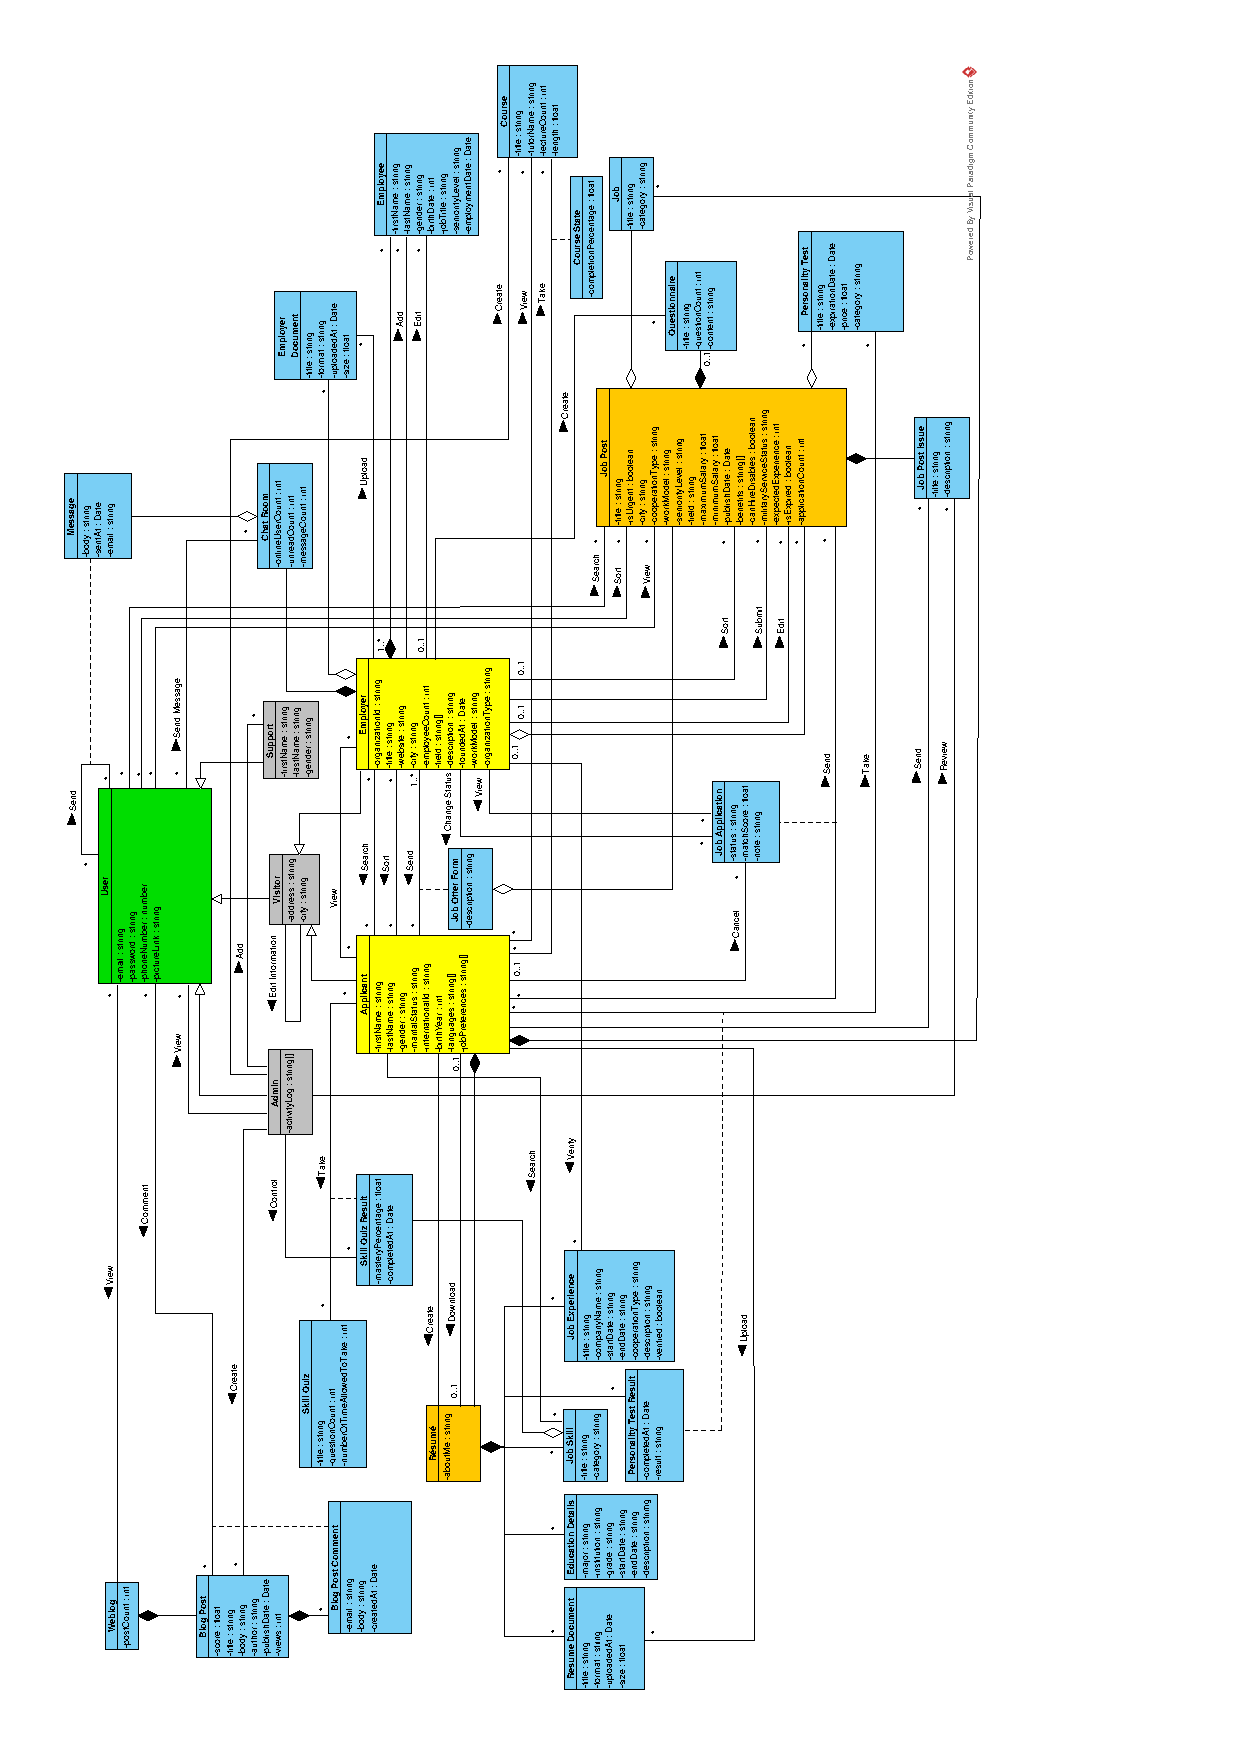
\includegraphics[width=1.2\textwidth, height=0.9\textheight]{files/Project_OOAD_Phase2_DiagramClass_V5_rotated}
		\caption{نمودار مدل دامنه}
		\label{fig:classdiagram}
	\end{figure}

	\newpage
	\subsubsection{مرور مدل دامنه}
	جهت شناسایی و تصحیح خطاها و موارد غیرعادی، مدل دامنه در دو جلسه یک ساعته توسط اعضا تیم مرور و بررسی شد. در این مرور مواردی از جمله در برداشتن بیشتر کلاس‌های مهم دامنه کاربرد، در برداشتن همه‌ روابط مهم دامنه کاربرد، شامل یک یا چند کلاس طراحی یا پیاده‌سازی بودن مدل دامنه، نمایش صفات مهم در کلاس‌ها، مناسب و قابل فهم بودن نام صفات و کلاس‌ها و روابط بررسی شدند.\\
	همچنین در آخر این جلسه با همفکری همه اعضای گروه، تصمیم بر اضافه کردن چند کلاس کاربردی جهت قابل فهم کردن مدل دامنه شد.

	\newpage
	\section{طراحی معماری}
	\subsection{شرح کلی}
	به سبک طراحی ساختار یک سیستم، شامل برقراری ارتباط و تعامل بین زیرسیستم‌ها و اجزای آن، معماری نرم‌افزاری یک سیستم یا زیرسیستم گفته می‌شود. طراحی معماری، یک فرایند تصمیم‌گیری برای تعیین معماری نرم‌افزار سیستم تحت توسعه است که می‌تواند به عنوان مجموعه‌ای از تصمیم‌های طراحی نیز تعریف گردد. معماری یک سیستم نرم‌افزاری، بر تعدادی از ویژگی‌های سیستم شامل کارایی، بهره‌وری، امنیت و قابلیت نگه‌داری بسیار مؤثر است و همچنین عامل تعیین کننده‌ای در طول چرخه عمر آن است.

	\subsection{فرآیند طراحی معماری}
	فرایند طراحی معماری برای یک سیستم یا زیرسیستم نرم‌افزاری، یک فرایند شناختی تصمیم گیری است. این فرایند باید عوامل زیادی را در نظر بگیرد چرا که نوع سیستمی که می‌خواهد توسعه داده شود و اهداف طراحی، بر انتخاب سبک معماری مؤثرند. یک سیستم متشکل از تعدادی زیرسیستم است که این زیرسیستم‌ها خود شامل زیرسیستم‌ها یا اجزای سطوح پایین‌تری هستند. از این رو طراحی معماری یک فرایند بازگشتی\footnote{Recursive} محسوب می‌شود. لازم است که فرایند طراحی به‌طور بازگشتی تا همه‌ی سطوح پایین‌تر این سلسله مراتب انجام بگیرد، تا جایی که اجزای قرار گرفته در برگ‌های سلسله مراتب به‌راحتی طراحی و پیاده‌سازی گردند. فرایند طراحی معماری شامل گام‌های زیر است که هر یک از آن‌ها در ادامه به اختصار توضیح داده خواهند شد.

	\begin{enumerate}
		\renewcommand{\labelenumi}{گام \arabic{enumi}.}
		\item
	تعیین اهداف طراحی
		\item
	تعیین نوع سیستم
		\item
	به کارگیری یک سبک معماری
		\item
	تبیین عملیات، واسط‌ها و رفتار تعاملی زیرسیستم‌ها
		\item
	بازبینی طراحی معماری
	\end{enumerate}

	\subsubsection{اهداف طراحی معماری}
	یک طراحی معماری خوب برای یک سیستم، لزوماً برای سیستم دیگر مناسب نیست. بنابراین، اهداف طراحی معماری برای سیستم در حال توسعه باید مشخص شود و برای هدایت فرایند طراحی به کار برده شود. یک هدف طراحی معماری، یک ویژگی یا جنبه‌ای از سیستم را که باید در زمان طراحی مورد نظر قرار بگیرد مشخص می‌کند. اهداف طراحی معماری این سیستم به شرح زیر است:

	\begin{itemize}
		\item
		سامانه باید در برابر تغییرات احتمالی در داده‌ها یا نیازمندی‌ها به گونه‌ای باشد که تا حد امکان نیاز به تغییرات مکرر در طراحی معماری آن به‌وجود نیاید.
		\item
سیستم باید توانایی پردازش داده‌ها با حجم بالا را داشته باشد.
		\item
		عملکرد سیستم باید مطابق با قیود در نظر گرفته شده باشد و از اطمینان زیادی برخوردار باشد.
		\item
		از آن جایی که اطلاعات حیاتی کاربران در سیستم نگهداری می‌شود، سیستم باید از داده‌ها در برابر دسترسی‌های غیرمجاز محافظت کند.
		\item
سیستم باید در برابر خطاهای احتمالی تحمل‌پذیر باشد.
		\item
این سامانه باید به تمام درخواست‌های کاربران پاسخ مناسب دهد.
		\item
		برای پشتیبانی از سیستم و احتمال تغییر در آن و نیز به روزرسانی سیستم، زیرسیستم‌ها باید به گونه‌ای تعیین شوند که مستقل از یکدیگر باشند یا وابستگی کمی به یکدیگر داشته باشند.
		\item
		سامانه نیاز به اعتبارسنجی اطلاعات ورودی توسط کاربر را دارد.
		\item
		سامانه نیاز به یک واحد کنترل، جهت کنترل سطوح دسترسی و نقش کاربران دارد.
	\end{itemize}

	\subsubsection{تعیین نوع سیستم}
	نوع یک سیستم، مدل‌سازی، تحلیل، طراحی، پیاده‌سازی و آزمون سیستم را به شدت تحت تاثیر خود قرار می‌دهد. به همین دلیل باید در زمان طراحی معماری نرم افزار برای یک سیستم، به نوع آن توجه نمود.
	با توجه به اهداف طراحی معماری ذکر شده و ویژگی‌های سیستم که عبارتند از:

	\begin{itemize}
		\item برقرای تعامل بین کاربر و سامانه به منظور انجام دنباله‌ای از درخواست‌ها
		\item کنشگرهای این سیستم انسان‌ها هستند و تعامل با کنشگر شروع می‌شود و به کنشگر نیز ختم می‌شود.
		\item تعامل تنها با یک کنشگر در فرایند مربوط به یک مورد کاربرد
		\item کنشگر خدماتی را درخواست می‌کند و سیستم این خدمات را فراهم می‌نماید که این ویژگی نوعی رابطه مشتری - خادم را تداعی می‌کند.
	\end{itemize}
	این سامانه یک سیستم تعاملی است و معماری آن باید متناسب با این نوع سیستم در نظر گرفته شود.

	\subsubsection{استفاده از سبک‌های معماری}
	انواع مختلف سیستم‌ها، به معماری‌های متفاوت نرم‌افزار نیازمندند. بنابراین باید با توجه به سیستم در حال توسعه، سبک معماری مناسب انتخاب شود.\\
	با توجه به اهداف طراحی معماری و تعاملی بودن این سیستم، مناسب‌ترین سبک معماری برای سیستم، معماری N لایه است.\\
	این سبک معماری اجزای سیستم را به لایه‌های نسبتاً مستقل با اتصال ضعیف، تقسیم می‌نماید. هر لایه یک وظیفه و عملکرد خوش‌تعریف دارد و تأثیرات بر لایه‌های دیگر را کاهش می‌دهد. تفکیک لایه‌ها اجازه‌ی مدیریت و دستیابی به هر لایه را به صورت مستقیم می‌دهد. همچنین این معماری مدیریت زیرساخت‌های نرم‌افزاری را ساده می‌کند. زمانی که معماری به چند لایه تقسیم می‌شود تغییراتی که ایجاد می‌شود ساده‌تر و کم هزینه‌تر از حالت معمول خواهد بود.\\
	این معماری در حالت معمول از لایه‌های زیر تشکیل می‌شود:
	\begin{enumerate}
		\item لایه نمایش\footnote{\lr{Presentation Layer}}:
		این لایه مسئول نمایش واسط گرافیکی کاربر و پاسخ‌های سیستم به کاربران است.
		\item لایه کسب و کار\footnote{\lr{Business Object Layer}}:
		این لایه مسئول پردازش تراکنش‌های کسب‌کار است که با موارد کاربرد نشان داده شده‌اند.
		\item لایه انباره ی مانا\footnote{\lr{Persistence Storage Layer}}:
		این لایه از اشیایی تشکیل می‌شود که عملیات مربوط به پایگاه داده مانند ذخیره و بازیابی اشیا را فراهم می‌نمایند.
		\item لایه ارتباط شبکه\footnote{\lr{Network Communication Layer}}:
		این لایه عملیات مربوط به ارتباطات شبکه را فراهم می‌سازد.
	\end{enumerate}
	\begin{figure}[H]
		\centering
		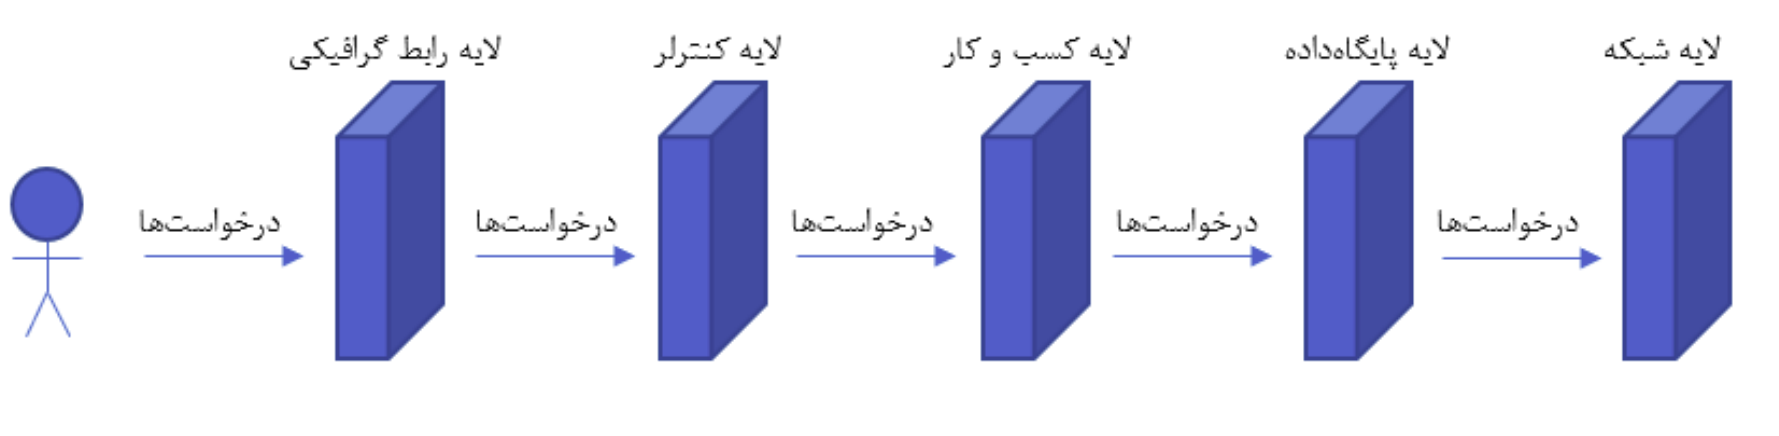
\includegraphics[width=0.9\linewidth]{files/2}
		\caption{تعامل لایه‌ها در معماری N لایه}
		\label{fig:2}
	\end{figure}

	\subsubsection{تعیین واسط‌ها و عملیات زیرسیستم‌ها}
	در این گام، واسط‌های بین زیرسیستم‌ها مشخص می‌گردند. ورودی و خروجی هر زیرسیستم شامل تعداد، انواع و ترتیب پارامترهای ورودی و خروجی در توصیف این واسط‌ها تعریف می‌گردند. به علاوه، رفتار تعاملی بین زیر سیستم‌ها (به معنای رشته پیام‌هایی که باید بین آن‌ها تبادل گردد) در این مرحله تعیین می‌شود.\\
	همچنین در این گام نیازمندی‌های نرم‌افزار و اهداف طراحی آن، به زیر سیستم‌ها و مؤلفه‌های معماری تخصیص داده می‌شود.
	معماری این سیستم از لایه‌های زیر تشکیل می‌شود که از بالا به پایین به صورت زیر می‌باشد:

	\begin{enumerate}
	\item \lr{\textbf{Presentation Layer}}
	این لایه اولین و بالاترین لایه است که در سایت نشان داده می‌شود. این لایه نمایش اطلاعات و اجزای گرافیک سیستم را بر عهده دارد و محتوا را به کاربران نهایی از طریق گرافیک نمایش می‌دهد. این لایه از طریق هر نوع دستگاه مانند کامپیوتر، لپ تاپ، موبایل و... قابل دسترس است. به طور کلی می‌توان کلاس‌های عضو این لایه را به دو زیرسیستم که خود جزئی از لایه نمایش هستند تقسیم نمود:

	\begin{itemize}
		\item \lr{\textbf{Interface User}}
	که رابط گرافیکی و ظاهر سامانه در آن پیاده‌سازی می‌شود.
		\item \lr{\textbf{Logic Presentation}}
		که مسئول برخی عملیات‌های محاسباتی در لایه نمایش است.
	\end{itemize}
	همچنین وظیفه انجام تعامل با کاربر و انتقال درخواست‌ها به لایه کسب و کار نیز بر عهده این لایه است.

	\item \lr{\textbf{Business Layer}}
	این لایه به منظور پردازش اطلاعات و اجرای محاسبات منطقی در سیستم ایجاد شده است. زیرسیستم‌های عضو این لایه به شرح زیر است:

	\begin{itemize}
		\item \lr{\textbf{Object Control}}
	پل ارتباطی بخش ظاهری و درونی سیستم است که هدف آن پیاده‌سازی API مناسب و بدون وابستگی به شیوه انجام عملیات در بخش
	  \lr{Business Logic}
	  است.

		\item \lr{\textbf{Business Logic}}
		 قلب یک برنامه کاربردی (نرم‌افزار) به حساب می‌آید. در این لایه اطلاعات دریافتی از لایه نمایش پردازش می‌شوند. همچنین، این زیرسیستم می‌تواند داده‌های لایه داده را نیز ویرایش یا حذف کند یا داده جدید به آن اضافه کند. لایه منطق با انجام پردازش دقیق، عملکرد اصلی برنامه را کنترل می‌کند. ارتباط با لایه داده نیز از طریق فراخوانی API\footnote{Application Programming Interface} انجام می‌شود.
	\end{itemize}

	\item \lr{\textbf{Data Layer}}
	در این لایه به هدف ذخیره و بازیابی اشیا، یک پایگاه‌داده\footnote{Database} مورد استفاده قرار می‌گیرد که داده‌های پردازش شده به وسيله لایه میانی به نام DBMS\footnote{Database Management System} در این لایه ذخیره و مدیریت خواهد شد. این لایه درخواست‌هایی از لایه بالاتر از خود دریافت می‌کند که این درخواست‌ها می‌توانند شامل عملیاتی مانند حذف، اضافه، ویرایش یا خواندن اطلاعات بر روی پایگاه داده باشد و در نهایت نتیجه را به لایه بالایی خود ارسال می‌کند. لایه نمایش و لایه داده نمی‌توانند مستقیماً با هم در ارتباط باشند.

	\item \lr{\textbf{Network Layer}}
	وظیفه این لایه است که چگونگی رسیدن داده‌ها به مقصد را تعیین کند. این لایه وظایفی از قبیل آدرس‌دهی، مسیریابی و پروتکل‌های منطقی را عهده‌دار است. این لایه مسیرهای منطقی\footnote{\lr{Logic Path}} بین مبدأ و مقصد ایجاد می‌کند که به اصطلاح مدارهای مجازی\footnote{\lr{Virtual Circuits}} نام‌گذاری می‌شوند. این مدارها باعث می‌شوند که هر بسته اطلاعاتی بتواند راهی برای رسیدن به مقصدش پیدا کند. لایه شبکه همچنین وظیفه مدیریت خطا در خود، ترتیب‌دهی بسته‌های اطلاعاتی و کنترل ازدحام را نیز برعهده دارد.

	\end{enumerate}

	\subsection{نمودار بسته\footnote{\lr{Package Diagram}}}
	برای استفاده از مزایای معماری نرم‌افزار برای فعالیت‌های توسعه، تیم نرم‌افزاری به راهی برای سازمان‌دهی مصنوعات تولید شده در طول فرایند توسعه نیازمند است. نمودار بسته، سازوکاری برای این امر فراهم می‌نماید.
	\begin{figure}[H]
		\centering
		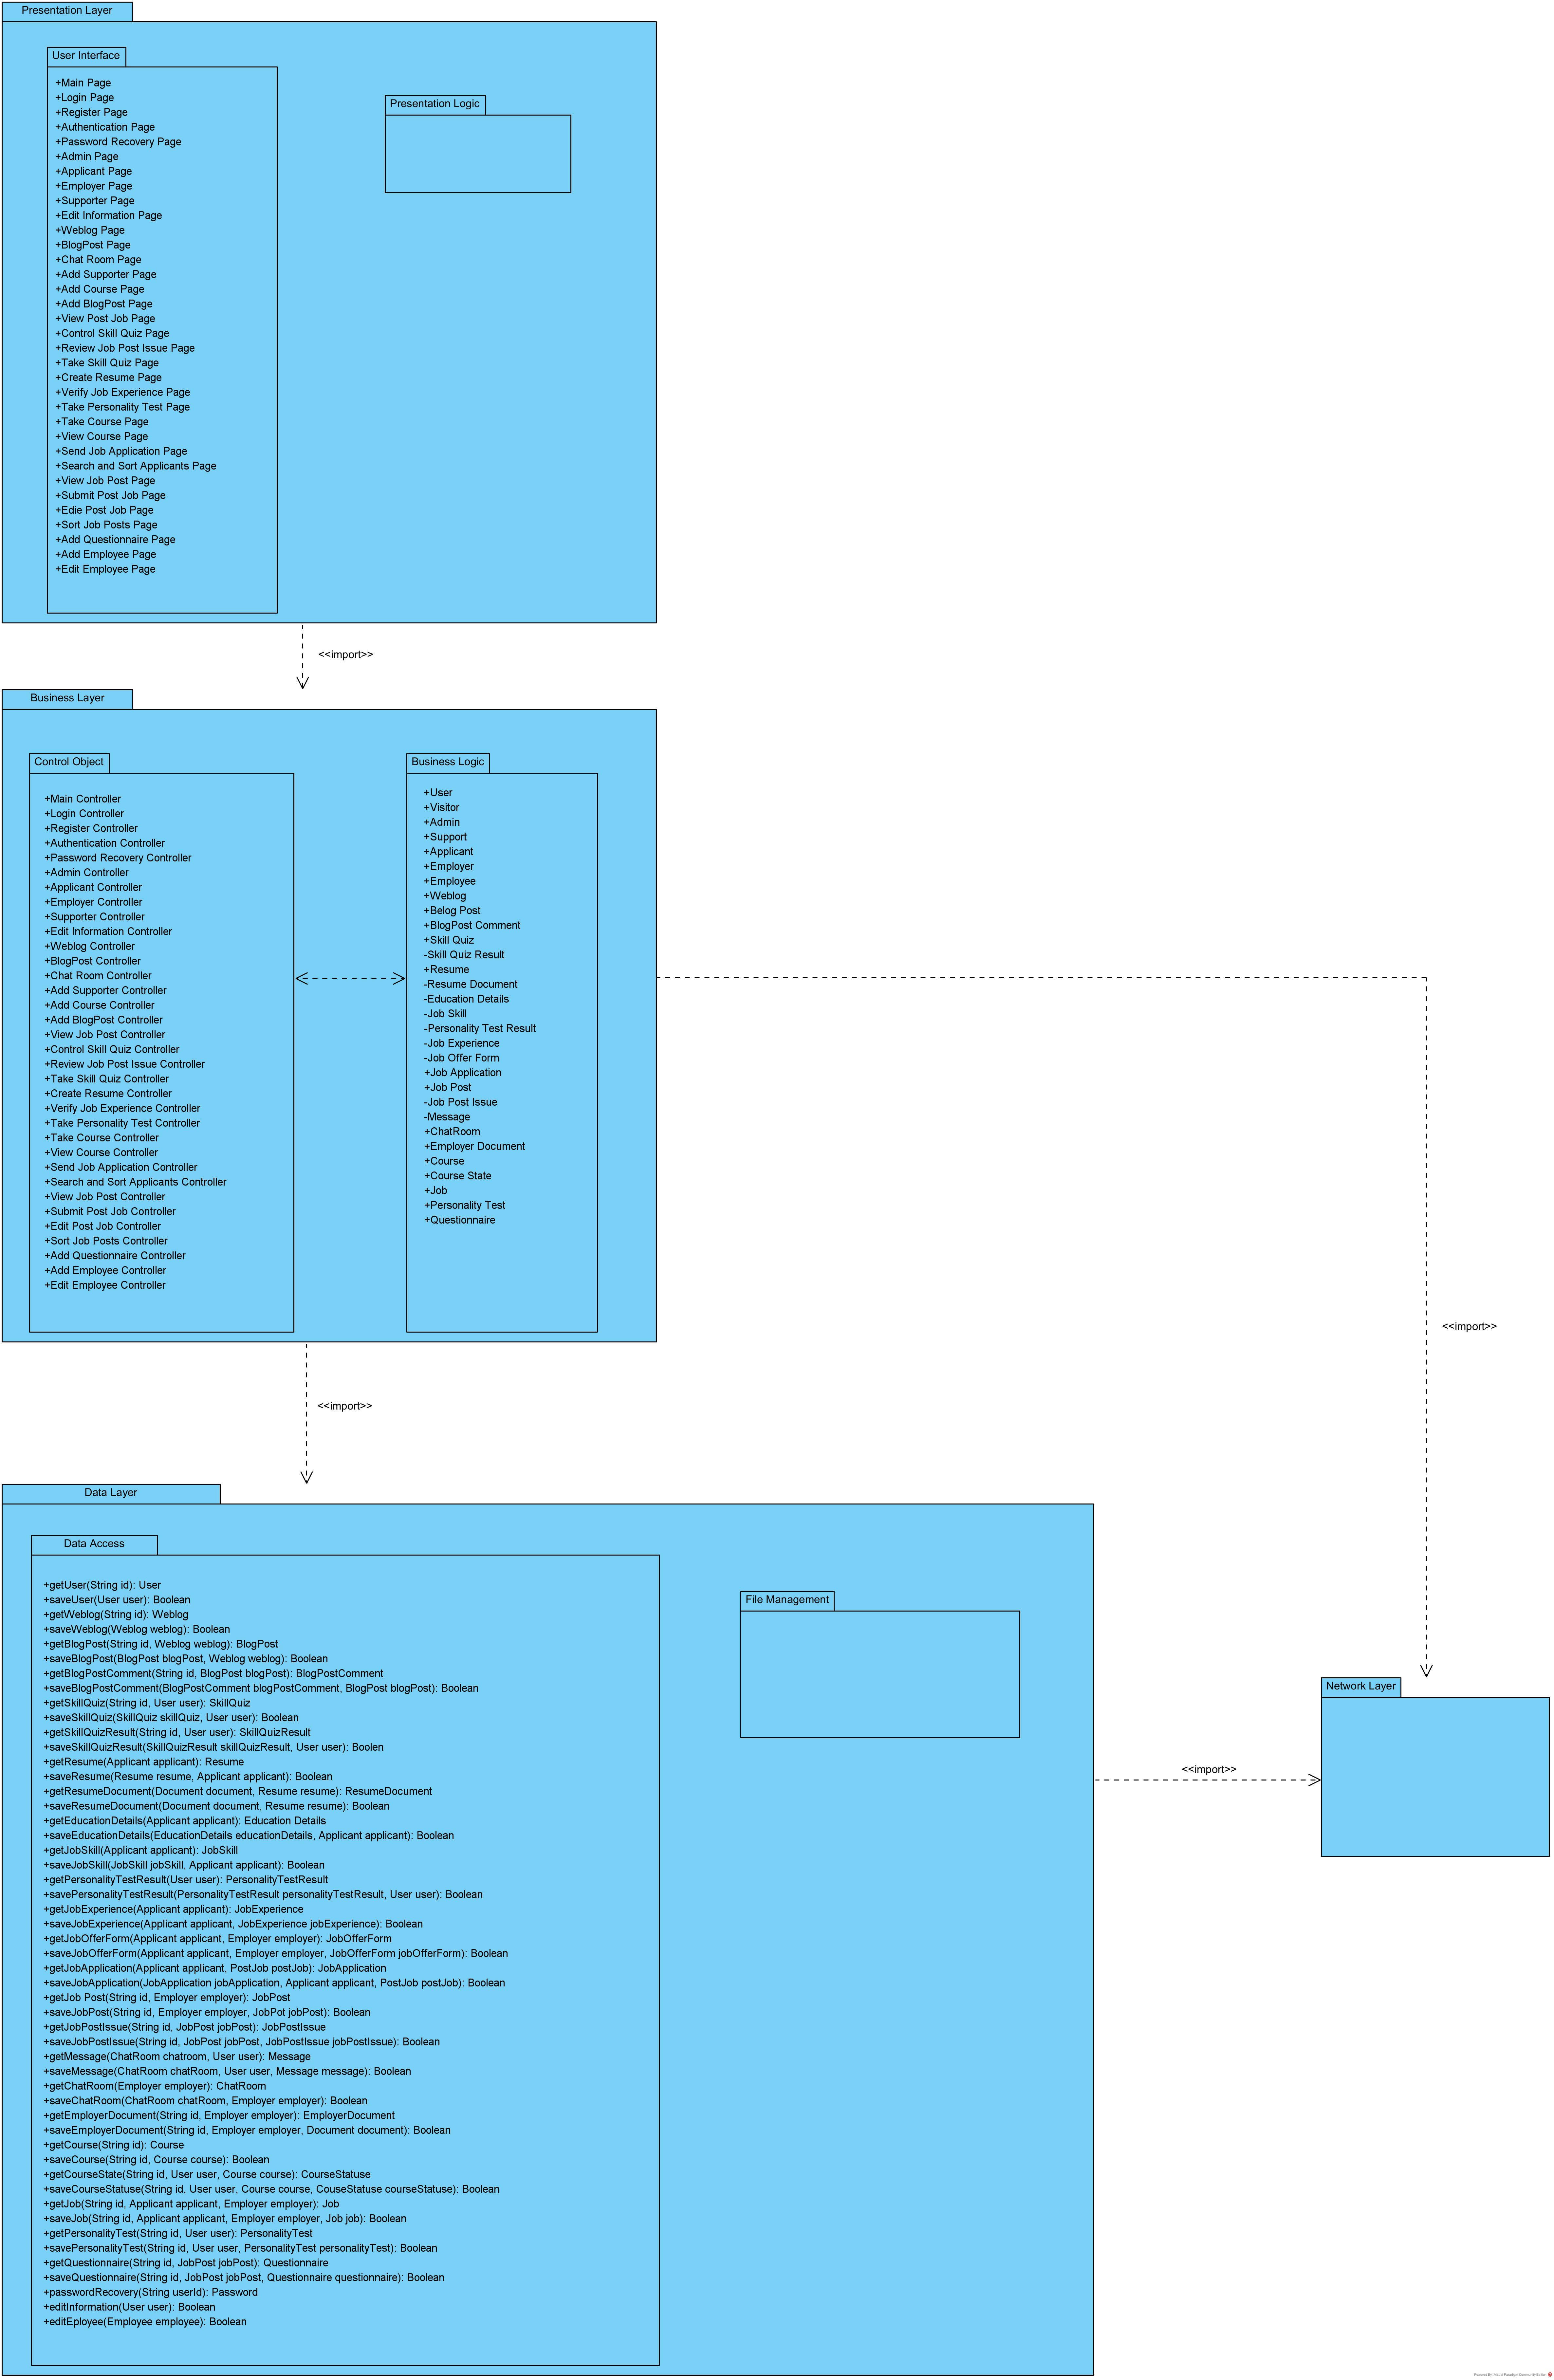
\includegraphics[width=0.5\linewidth]{files/Project_OOAD_Phase2_PackageDiagram}
		\caption{نمودار بسته}
		\label{fig:packagediagram}
	\end{figure}

	\subsection{اعمال قوانین طراحی نرم‌افزار}
	قوانین طراحی نرم‌افزار، قوانین تایید شده‌ای هستند که اعمال صحیح آن‌ها در طراحی نرم‌افزار، می‌تواند کیفیت و بهره‌وری نرم‌افزار را به شدت افزایش دهد و هزینه‌های نگه‌داری آن را نیز کاهش دهد؛ لذا اعمال این قوانین برای غلبه بر مشکلات طراحی ضروری بوده و در ادامه تعریف می‌شوند.
	\subsubsection{طراحی برای تغییر}
	با در نظر گرفتن زیرسیستم‌های سامانه به صورت مجزا و معماری چند لایه، وابستگی بخش‌های مختلف به یکدیگر به حداقل رسیده و امکان تغییر و بروزرسانی در هر یک از این بخش‌ها به ساده‌ترین حالت ممكن است و باعث بروز نگرانی برای تغییر در سایر بخش‌ها نمی‌شود.\\
	به عنوان مثال تغییر در لایه پایگاه داده در سامانه با در نظر گرفتن چند لایه بودن معماری، به راحتی قابل انجام است و هیچ گونه الزامی به ایجاد تغییر در سایر لایه‌ها نخواهد داشت.
	\subsubsection{جداسازی دغدغه‌ها}
	با توجه به اینکه تمرکز همزمان بر روی تمام بخش‌های سیستم باعث بروز مشکلات بسیاری در مراحل پیاده‌سازی می‌شود، قانون جداسازی ‌دغدغه‌ها می‌تواند به این امر کمک کند.\\
	طبق این قانون با در نظر گرفتن مسئله طراحی نرم‌افزار باید آن را در دو سطح در نظر گرفت، در سطح بالاتر چگونگی انجام فرایند کلی طراحی و در سطح پایین‌تر چگونگی طراحی اجزا و مولفه‌های سیستم، در واقع طراحی نرم‌افزار به هر دو فرایند طراحی و محصول طراحی توجه می‌کند. دید فرایند کلی طراحی به ما می‌گوید که باید بر یک جنبه از کل فرایند طراحی تمرکز کنیم و از جنبه‌های دیگر چشم‌پوشی کنیم.

	\begin{itemize}
		\item
		لایه واسط گرافیکی باید بر نمایش اطلاعات به کاربر نهایی تمرکز نماید.
		\item
		لایه پایگاه داده باید بر ذخیره و بازیابی اطلاعات تمرکز کند.
		\item
		لایه کسب و کار به پردازش تراکنش‌های کسب و کار می‌پردازد.
		\item
		لایه شبکه عملیات‌های مربوط به ارتباطات شبکه را فراهم می‌سازد.
	\end{itemize}
	این نیازها با استفاده از سبک‌های معماری چند لایه برآورده می‌شوند. استفاده از قانون جداسازی دغدغه‌ها برای طراحی معماری به این معنا است که مسئولیت‌های مربوط به دغدغه‌های مختلف، به زیر سیستم‌های مختلف اختصاص داده شود. این کار به چسبندگی عملیاتی بالا منجر خواهد شد و فهم و استفاده مجدد از زیر سیستم‌ها را آسان‌تر خواهد کرد.
	\subsubsection{پنهان‌سازی اطلاعات}
	قانون پنهان‌سازی اطلاعات، نخستین بار توسط دیوید پارناس\footnote{\lr{David Parnas}} به عنوان یک قانون طراحی معرفی گردید. مطابق این قانون، جزئیات پیاده‌سازی یک بدنه‌ی نرم‌افزاری، برای کاهش اثرات تغییر آن بر سایر قسمت‌های نرم‌افزاری، محافظت می‌شود. در این سیستم این امر با اختصاصی کردن داده‌های یک کلاس و ثابت نگه‌داشتن واسط آن کلاس انجام می‌‌گردد. این کار به شکل کارآمدی، اثرات موجی و پیامدهای تغییرات صورت گرفته در داده‌ساختارها و پیاده‌سازی توابع را در این سیستم، کاهش می‌دهد. به‌دلیل وجود معماری چند لایه و پنهان‌سازی برخی اجزای لایه از لایه‌های دیگر، رعایت کپسوله‌سازی\footnote{\lr{Encapsulation}} و شی‌گرایی\footnote{\lr{Object Oriented}} در این سامانه، اثرات تغییرات این گونه اجزا بر بخش‌های دیگر سیستم به حداقل رسیده است و این اصل به خوبی در این سیستم به کار برده شده است.
	\subsubsection{چسبندگی زیاد}
	مطابق این قانون، طراحی پیمانه‌ها لازم است به گونه‌ای باشد که توابع هر‌کدام، بیشترین درجه‌ی ارتباط با مسئولیت اصلی آن پیمانه را دارا باشد. در این سیستم با توجه به معماری چند لایه، مولفه‌ها و کلاس‌های هر زیرسیستم به مسئولیت‌های آن مرتبط است.

	\subsubsection{جفت‌شدگی کم}
	همان‌گونه که در قانون طراحی برای تغییر ذکر شد، زیرسیستم‌های سیستم اصلی به گونه‌ای انتخاب و طراحی شده‌اند که کمترین ارتباط را با یکدیگر داشته باشند. ارتباط کم بین این زیرسیستم‌ها باعث کاهش اثرات زمان اجرا می‌گردد.
	در معماری چند لایه که برای این سیستم انتخاب شده است، لایه‌ها جفت‌شدگی کمی دارند. هر لایه عملیات خود را به صورت مستقل انجام می‌دهد و نتایج خود را از طریق واسط‌ها در قالب خروجی به بقیه زیرسیستم‌ها منتقل می‌کند.

	\subsubsection{ساده و احمقانه فرض کن}
	به کارگیری این قانون در طراحی معماری، به معنای طراحی معماری برای استفاده از اشیای نادان است. شئ نادان به شئ‌ای تلقی می‌شود که ساده‌گیر است و صرفا روش انجام یک کار را می‌داند. این قانون منجر به تولید طراحی‌های ساده، سرراست و قابل فهم می‌شود. زیرسیستم‌ها در این سامانه به صورت اشیای نادان در نظر گرفته شده‌اند به این معنا که هر لایه به جز انجام یک وظیفه خاص، از دیگر وظایف یا مدیریت‌ها اطلاع ندارد.

	\newpage
	\section{استخراج مورد کابردها و مدل‌سازی تعامل کنشگر-سیستم}
	\subsection{شناسایی و تعیین قلمرو مورد کاربردها}
	در این بخش به استخراج مورد کاربردها و تعیین قلمرو می‌پردازیم. مورد کاربردها، نیازمندی‌ها را پالایش کرده و یک طراحی از رفتار سیستم را مشخص می‌کنند. قلمرو هر مورد کاربرد نیز مشخص می‌کند که آن مورد کاربرد کی شروع می‌شود؟ کنش کنشگر کجا اتفاق می‌افتد؟ مورد کاربرد کی تمام می‌شود؟\\
	لیست مورد کاربردهای سطح بالا به شرح زیر است:
	\begin{enumerate}
		\item
		ثبت‌نام اولیه (کنشگر:‌کاربر، سیستم: سامانه کارا)\\
		TUCBW کاربر در صفحه اصلی، روی پیوند «ثبت‌نام» کلیک می‌کند.\\
		TUCEW کاربر نتیجه ثبت‌نام خود را مشاهده می‌کند.\\

		\item
		ورود کاربران (کنشگر:‌کاربر، سیستم: سامانه کارا)\\
		TUCBW کاربر در صفحه اصلی، روی پیوند «ورود» کلیک می‌کند. \\
		TUCEW کاربر نتیجه ورود خود را مشاهده می‌کند.\\

		\item
		بازیابی رمز عبور (کنشگر:‌کاربر، سیستم: سامانه کارا)\\
		TUCBW کاربر در صفحه ورود، روی دکمه «بازیابی رمز عبور» کلیک می‌کند.\\
		TUCEW کاربر نتیجه بازیابی رمز عبور خود را طبق یک پیام مناسب مشاهده می‌کند.\\

		\item
	تعریف دوره‌های آموزشی (کنشگر:‌مدیر، سیستم: سامانه کارا)\\
		TUCBW  مدیر در صفحه کاربری خود، روی گزینه «تعریف دوره آموزشی» کلیک می‌کند.\\
		TUCEW مدیر پیام «دوره جدید تعریف شد.» را مشاهده می‌کند.\\

		\item
		مشاهده اسناد و اطلاعات محرمانه کاربران (کنشگر:‌مدیر، سیستم: سامانه کارا)\\
		TUCBW مدیر در صفحه کاربری خود، روی پیوند «اسناد و اطلاعات کاربر» کلیک می‌کند.\\
		TUCEW مدیر اسناد و اطلاعات کاربر مورد نظر را مشاهده می‌کند.\\

		\item
		رد یا تایید مدارک آپلود شده هنگام ثبت‌نام (کنشگر:‌مدیر، سیستم: سامانه کارا)\\
		TUCBW مدیر در صفحه کاربری خود، روی پیوند «مدارک آپلود شده» کلیک می‌کند.\\
		TUCEW مدیر نتیجه کنترل خود را مشاهده می‌کند.\\

		\item
		سلب دسترسی کاربران (کنشگر:‌مدیر، سیستم: سامانه کارا)\\
		TUCBW مدیر در صفحه کاربران، روی گزینه «سلب دسترسی کاربر» کلیک می‌کند.\\
		TUCEW مدیر پیام «سلب دسترسی این کاربر با موفقیت انجام شد.» را مشاهده می‌کند.\\

		\item
		تعریف حساب کاربری با عنوان «پشتیبان سامانه» (کنشگر:‌مدیر، سیستم: سامانه کارا)\\
		TUCBW مدیر در صفحه کاربری خود، روی گزینه «تعریف پشتیبان» کلیک می‌کند.\\
		TUCEW مدیر پیام «پشتیبان جدید تعریف شد.» را مشاهده می‌کند.\\

		\item
		مشاهده حقوق تخمین زده شده (کنشگر:‌کاربر، سیستم: سامانه کارا)\faStar\\
		TUCBW کاربر در صفحه اصلی، روی «پیوند ماشین حساب حقوق» کلیک می‌کند.\\
		TUCEW کاربر یک حقوق تخمین زده شده را مشاهده می‌کند.\\

		\item
	مشاهده پیام‌های خصوصی (کنشگر:‌کاربر، سیستم: سامانه کارا)\\
		TUCBW کاربر در صفحه اصلی، روی پیوند پیام خصوصی کلیک می‌کند.\\
		TUCEW کاربر پیام‌های خصوصی خود را مشاهده می‌کند.\\

		\item
		ارسال پیام خصوصی (کنشگر:‌کاربر، سیستم: سامانه کارا)\faStar\\
		TUCBW کاربر روی پیوند «پیام خصوصی» در صفحه اصلی کلیک می‌کند.\\
		TUCEW کاربر نتیجه ارسال پیام خصوصی خود را مشاهده می‌کند.\\

		\item
		جستجو سریع در آگهی‌ها (کنشگر:‌کاربر، سیستم: سامانه کارا)\\
		TUCBW کاربر در صفحه اصلی روی پیوند جستجوی سریع کلیک می‌کند.\\
		TUCEW کاربر نتایج جستجوی سریع خود را مشاهده می‌کند.\\

		\item
		جستجو پیشرفته در آگهی‌ها (کنشگر:‌کاربر، سیستم: سامانه کارا)\faStar\\
		TUCBW کاربر در صفحه اصلی، روی پیوند «جستجوی پیشرفته» در صفحه اصلی کلیک می‌کند.\\
		TUCEW کاربر نتیجه جستجوی خود را مشاهده می‌کند.\\

		\item
		تکمیل اطلاعات شخصی  (اجباری) (کنشگر:‌کاربر بازدید‌کننده، سیستم: سامانه کارا)\\
		TUCBW کاربر بازدید‌کننده در صفحه کاربری خود، روی پیوند اطلاعات شخصی کلیک می‌کند.\\
		TUCEW کاربر بازدید‌کننده پیام «اطلاعات شما با موفقیت تکمیل شد.» را مشاهده می‌کند.\\

		\item
		ویرایش اطلاعات شخصی (کنشگر:‌کاربر بازدید‌کننده، سیستم: سامانه کارا)\\
		TUCBW کاربر بازدید‌کننده در صفحه کاربری خود، روی پیوند «اطلاعات شخصی» کلیک می‌کند.\\
		TUCEW کاربر بازدید‌کننده پیام «اطلاعات شما با موفقیت ویرایش شد.» را مشاهده می‌کند.\\

		\item
		مشاهده آگهی‌های شغلی (کنشگر:‌کاربر بازدید‌کننده، سیستم: سامانه کارا)\\
		TUCBW کاربر بازدید‌کننده در صفحه آگهی‌های شغلی روی «عنوان آگهی شغلی» کلیک می‌کند.\\
		TUCEW بازدید‌کننده صفحه‌ای شامل اطلاعات مربوط به  آگهی شغلی مورد‌نظر را مشاهده می‌کند.\\

		\item
		نشان کردن آگهی (کنشگر:‌کارجو، سیستم: سامانه کارا)\\
		TUCBW کارجو در صفحه آگهی، روی دکمه «نشان کردن» کلیک می‌کند.\\
		TUCEW کارجو پیام «آگهی با موفقیت نشان شد» را مشاهده می‌کند.\\

		\item
		ارسال درخواست شغلی (کنشگر:کارجو، سیستم: سامانه کارا)\faStar\\
		TUCBW کارجو در صفحه آگهی، روی گزینه «ارسال درخواست شغلی» کلیک می‌کند.\\
		TUCEW کارجو نتیجه ارسال درخواست شغلی خود را در قالب پیام مناسب مشاهده می‌کند.\\

		\item
		لغو ارسال رزومه  (کنشگر:‌کارجو، سیستم: سامانه کارا)\\
		TUCBW کارجو در صفحه رزومه‌های ارسال شده، روی دکمه «لغو رزومه» کلیک می‌کند.\\
		TUCEW کارجو نتیجه‌ لغو رزومه را مشاهده می‌کند.\\

		\item
		انجام آزمونک‌ صحت‌سنجی (کنشگر:‌کارجو، سیستم: سامانه کارا)\\
		TUCBW کارجو در صفحه کاربری خود، روی دکمه «شروع آزمونک صحت‌سنجی» کلیک می‌کند.\\
		TUCEW کارجو نتیجه‌ آزمونک صحت‌سنجی را مشاهده می‌کند.\\


		\item
		ثبت مشکل آگهی (کنشگر:‌کارجو، سیستم: سامانه کارا)\faStar\\
		TUCBW کارجو در صفحه آگهی، روی «ثبت مشکل» کلیک می‌کند.\\
		TUCEW کارجو پیغام مناسب را مشاهده می‌کند.\\

		\item
		مشاهده صفحه کارفرما (کنشگر:‌کارجو، سیستم: سامانه کارا)\\
		TUCBW کارجو در صفحه آگهی، روی عنوان کارفرما کلیک می‌کند.\\
		TUCEW کارجو صفحه‌ای شامل اطلاعات مربوط به کارفرما را مشاهده می‌کند.\\

		\item
		انجام آزمون‌ شخصیتی (کنشگر:‌کارجو، سیستم: سامانه کارا)\\
		TUCBW کارجو در صفحه آزمون شخصیتی، روی دکمه «شروع آزمون شخصیتی» کلیک می‌کند.\\
		TUCEW کارجو نتیجه‌ آزمون شخصیتی را مشاهده می‌کند.\\

		\item
		ساخت رزومه (کنشگر:‌کارجو، سیستم: سامانه کارا)\faStar\\
		TUCBW کارجو در صفحه کاربری خود، روی گزینه «ساخت رزومه» کلیک می‌کند.\\
		TUCEW کارجو نتیجه ساخت رزومه خود را مشاهده می‌کند.\\

		\item
		مشاهده رزومه (کنشگر:‌کارجو، سیستم: سامانه کارا)\\
		TUCBW کارجو در صفحه کاربری خود، روی دکمه «مشاهده رزومه» کلیک می‌کند.\\
		TUCEW کارجو صفحه‌ای شامل اطلاعات رزومه خود را مشاهده می‌کند.\\

		\item
		ثبت‌نام دوره‌ آموزشی (کنشگر:‌کارجو، سیستم: سامانه کارا)\\
		TUCBW کارجو در صفحه دوره، روی پیوند «شروع دوره» کلیک می‌کند.\\
		TUCEW کارجو پیغام «ثبت‌نام دوره با موفقیت انجام شد» را مشاهده می‌کند.\\

		\item
		ثبت حقوق تخمین زده شده (کنشگر:‌کارجو، سیستم: سامانه کارا)\\
		TUCBW کاربر در صفحه اصلی، روی پیوند «ماشین حساب حقوق» کلیک می‌کند.\\
		TUCEW کاربر پیغام «اطلاعات وارد شده با موفقیت ثبت شد» را مشاهده می‌کند.\\

		\item
		ثبت آگهی (کنشگر:‌کارفرما، سیستم: سامانه کارا)\faStar\\
		TUCBW کارفرما در صفحه کاربری خود، روی گزینه «ثبت آگهی» کلیک می‌کند.\\
		TUCEW کارفرما نتیجه ساخت آگهی خود را مشاهده می‌کند.\\

		\item
		ویرایش آگهی (کنشگر:‌ کارفرما، سیستم: سامانه کارا)\\
		TUCBW کارفرما در صفحه آگهی، روی پیوند «ویرایش» کلیک می‌کند.\\
		TUCEW کارفرما پیغام «آگهی با موفقیت ویرایش شد» را مشاهده می‌کند.\\

		\item
		طبقه بندی آگهی‌های ثبت شده (کنشگر:‌ کارفرما، سیستم: سامانه کارا)\\
		TUCBW کارفرما در صفحه آگهی‌های خود، روی گزینه «طبقه‌بندی آگهی» کلیک می‌کند.\\
		TUCEW کارفرما آگهی‌های «طبقه‌بندی شده» را مشاهده می‌کند.\\

		\item
		مشاهده آگهی‌های ثبت شده کارفرما (کنشگر:‌کارفرما، سیستم: سامانه کارا)\\
		TUCBW کارفرما در صفحه کاربری خود، روی گزینه «آگهی‌های ثبت شده» کلیک می‌کند.\\
		TUCEW کارفرما آگهی‌های ثبت شده را مشاهده می‌کند.\\

		\item
		مشاهده صفحه کارجو (کنشگر:‌کارفرما، سیستم: سامانه کارا)\\
		TUCBW کارفرما در صفحه رزومه کارجو، روی نام کاربری کارجو کلیک می‌کند.\\
		TUCEW کارفرما صفحه کاربری کارجو را مشاهده می‌کند.\\

		\item
		جستجو در بانک رزومه (کنشگر:‌کارفرما، سیستم: سامانه کارا)\\
		TUCBW کارفرما در صفحه کاربری خود،‌ روی گزینه «جستجو در بانک رزومه» کلیک می‌کند.\\
		TUCEW کارفرما نتایج جستجو را مشاهده می‌کند.\\

		\item
		ارسال پیشنهاد همکاری (کنشگر: کارفرما، سیستم: سیستم کارا)\\
		TUCBW کارفرما در صفحه کاربری کارجو، روی گزینه «ارسال پیشنهاد همکاری» کلیک می‌کند.\\
		TUCEW کارفرما پیام «پیشنهاد همکاری برای کارجو با موفقیت ارسال شد.» را مشاهده می‌کند.\\

		\item
		بارگیری رزومه کارجویان (کنشگر: کارفرما، سیستم: سیستم کارا)\\
		TUCBW کارفرما در صفحه رزومه کارجو، روی گزینه «بارگیری رزومه» کلیک می‌کند.\\
		TUCEW کارفرما پیام «رزومه با موفقیت بارگیری شد.» را مشاهده می‌کند.\\

		\item
		تغییر سطح ارشدیت توسط کارفرما (کنشگر: کارفرما، سیستم: سامانه کارا)\\
		TUCBW کارفرما در صفحه تغییرات پیشنهادی، روی گزینه «اعمال تغییرات» کلیک می‌کند.\\
		TUCEW کارفرما نتایج تغییرات اعمال شده را مشاهده می‌کند.\\

		\item
		مشاهده فهرست تغییرات پیشنهادی سطح ارشدیت (کنشگر: کارفرما ، سیستم: سامانه کارا)\\
		TUCBW کارفرما در صفحه کارمندان، روی گزینه «به‌روزرسانی سطح ارشدیت» کلیک می‌کند.\\
		TUCEW کارفرما نتایج پیشنهادی سیستم را مشاهده می‌کند.\\

		\item
		مشاهده فهرست کارجویان پیشنهادی (کنشگر: کارفرما، سیستم: سامانه کارا)\\
		TUCBW کارفرما در صفحه آگهی، روی گزینه «کارجویان پیشنهادی» کلیک می‌کند.\\
		TUCEW کارفرما فهرست کارجویان پیشنهادی را مشاهده می‌کند.\\

		\item
		ثبت اعلان در سامانه (کنشگر: مدیر، سیستم: سامانه کارا)\\
		TUCBW مدیر در صفحه کاربری خود، روی گزینه «ثبت اعلان» کلیک می‌کند.\\
		TUCEW مدیر پیام «اعلان با موفقیت ثبت شد» را مشاهده می‌کند.\\

		\item
		مشاهده لیست آگهی‌های شغلی پیشنهادی (کنشگر: کارجو، سیستم: سامانه کارا)\\
		TUCBW کارجو در صفحه اصلی، روی پیوند آگهی‌های شغلی کلیک می‌کند.\\
		TECEW کارجو نتیجه پیشنهاد آگهی‌های شغلی را مشاهده می‌کند.\\
	\end{enumerate}

	\subsection{ترسیم نمودار مورد کاربرد}
	در این بخش برای نمایش بهتر مورد کاربردها نمودار مورد کاربرد آن‌ها رسم شدند. برای هر کدام از این نمودارها زیرسیستمی در نظر گرفته شده است و مورد کاربرد‌هایی به آن اختصاص داده شده است. قابل ذکر است که این نمودارها توسط نرم‌افزار
	\lr{Visual Paradigm}
	 رسم شده‌اند. مورد کاربرد‌ها را طبق نقش آن‌ها افراز می‌کنیم. مورد کاربردهای مربوط به زیر سیستم کاربر، بازدیدکننده، کارجو، کارفرما و مدیر به شرح زیر است:

	\begin{figure}[H]
		\centering
		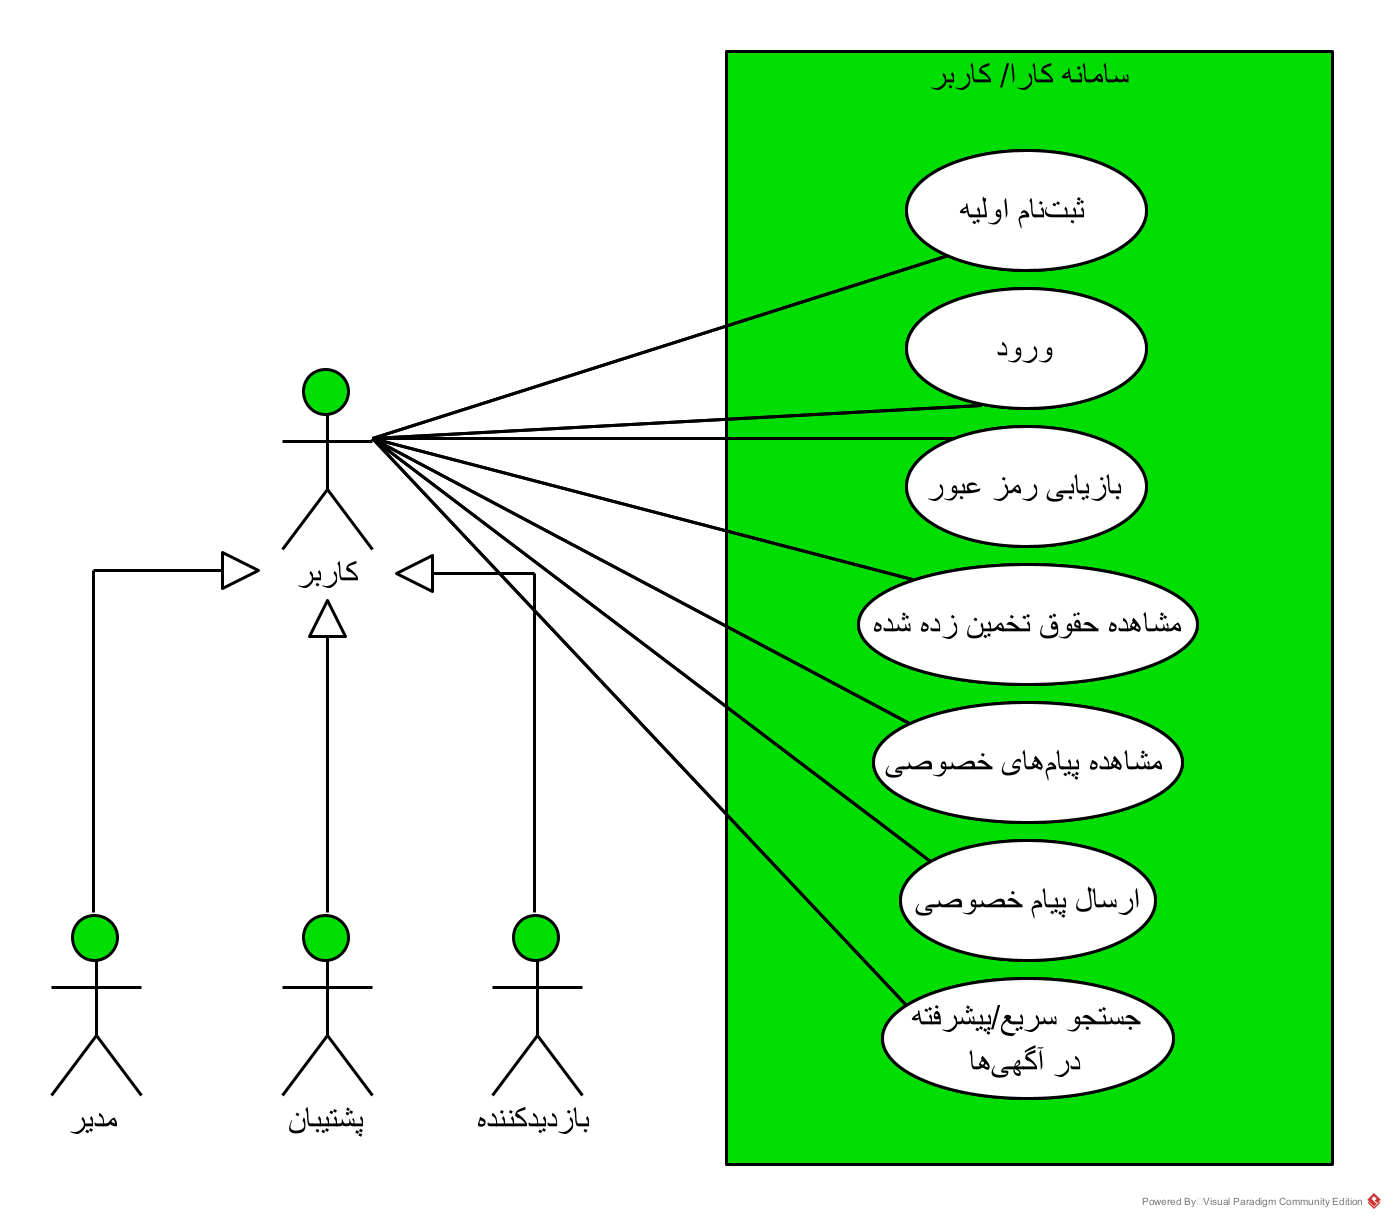
\includegraphics[width=0.7\linewidth]{files/UseCaseDiagram/UseCase_User}
		\caption{نمودار مورد کاربرد سامانه کارا برای کاربر}
		\label{fig:usecaseuser}
	\end{figure}
	\begin{figure}[H]
		\centering
		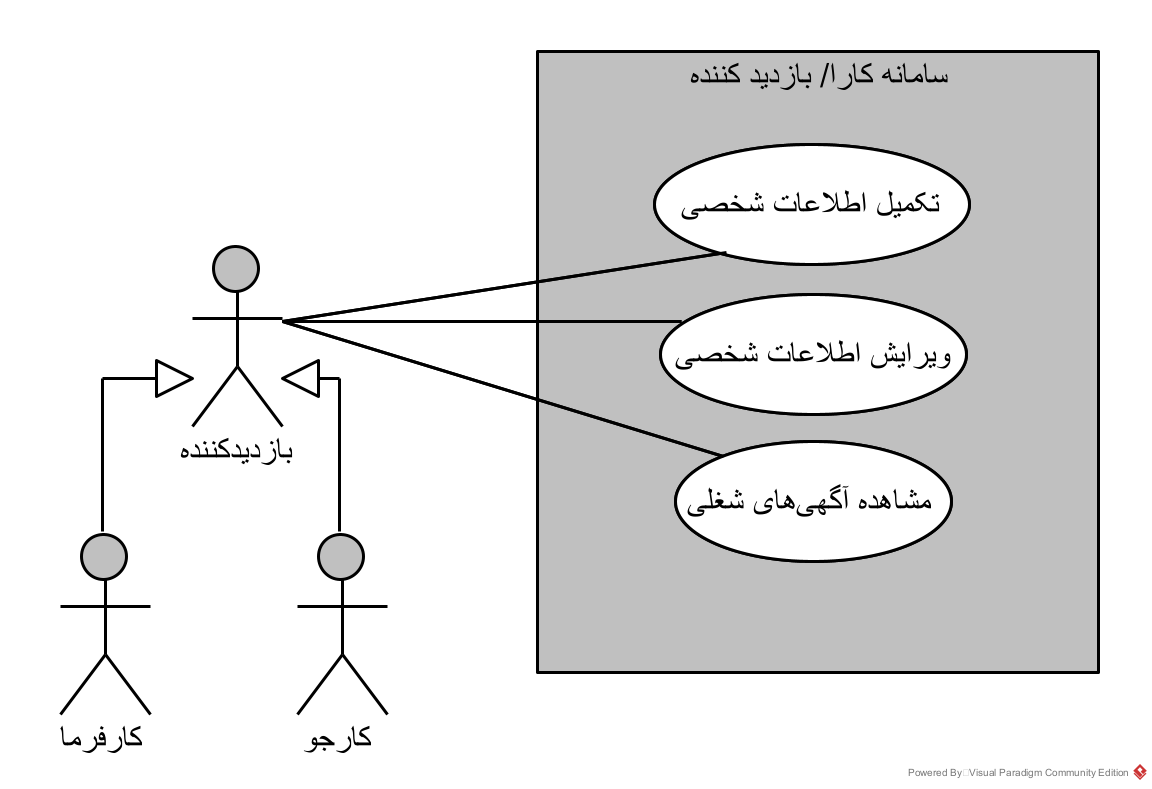
\includegraphics[width=0.7\linewidth]{files/UseCaseDiagram/UseCase_Visitor}
		\caption{نمودار مورد کاربرد سامانه کارا برای بازدیدکننده}
		\label{fig:usecasevisitor}
	\end{figure}
	\begin{figure}[H]
		\centering
		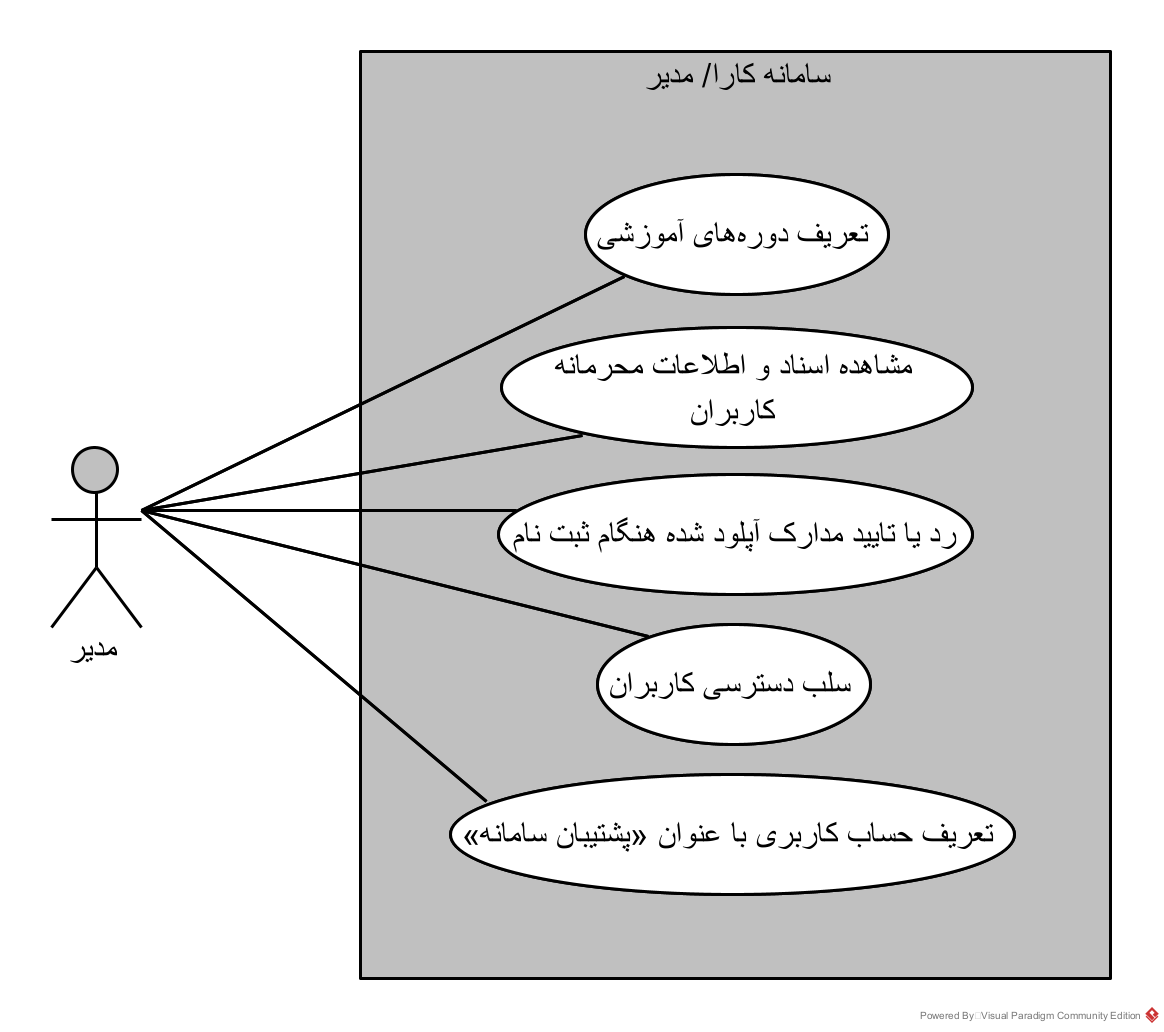
\includegraphics[width=0.7\linewidth]{files/UseCaseDiagram/UseCase_Admin}
		\caption{نمودار مورد کاربرد سامانه کارا برای مدیر}
		\label{fig:usecaseadmin}
	\end{figure}
	\begin{figure}[H]
		\centering
		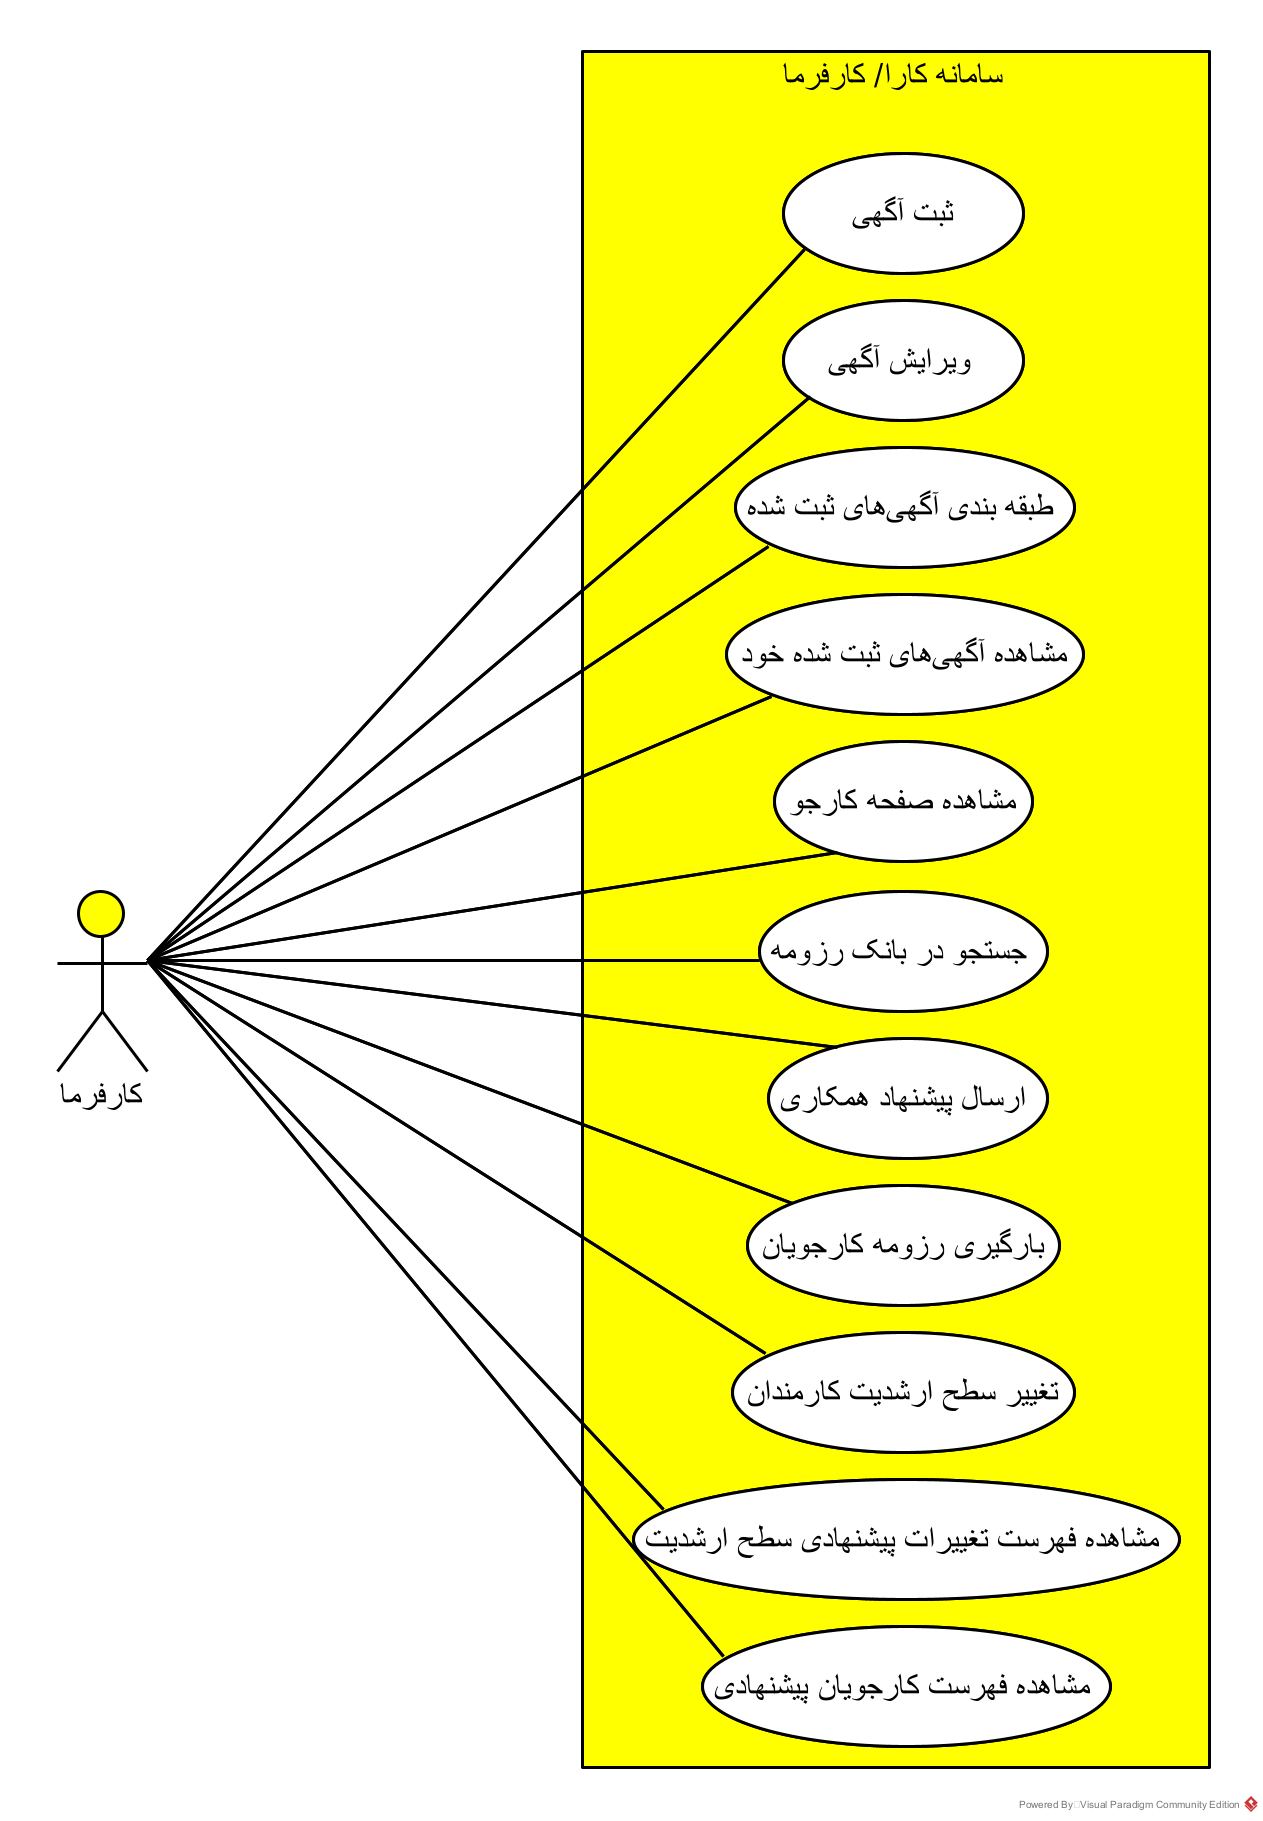
\includegraphics[width=0.7\linewidth]{files/UseCaseDiagram/UseCase_Applicant}
		\caption{نمودار مورد کاربرد سامانه کارا برای کارجو}
		\label{fig:usecaseapplicant}
	\end{figure}
	\begin{figure}[H]
		\centering
		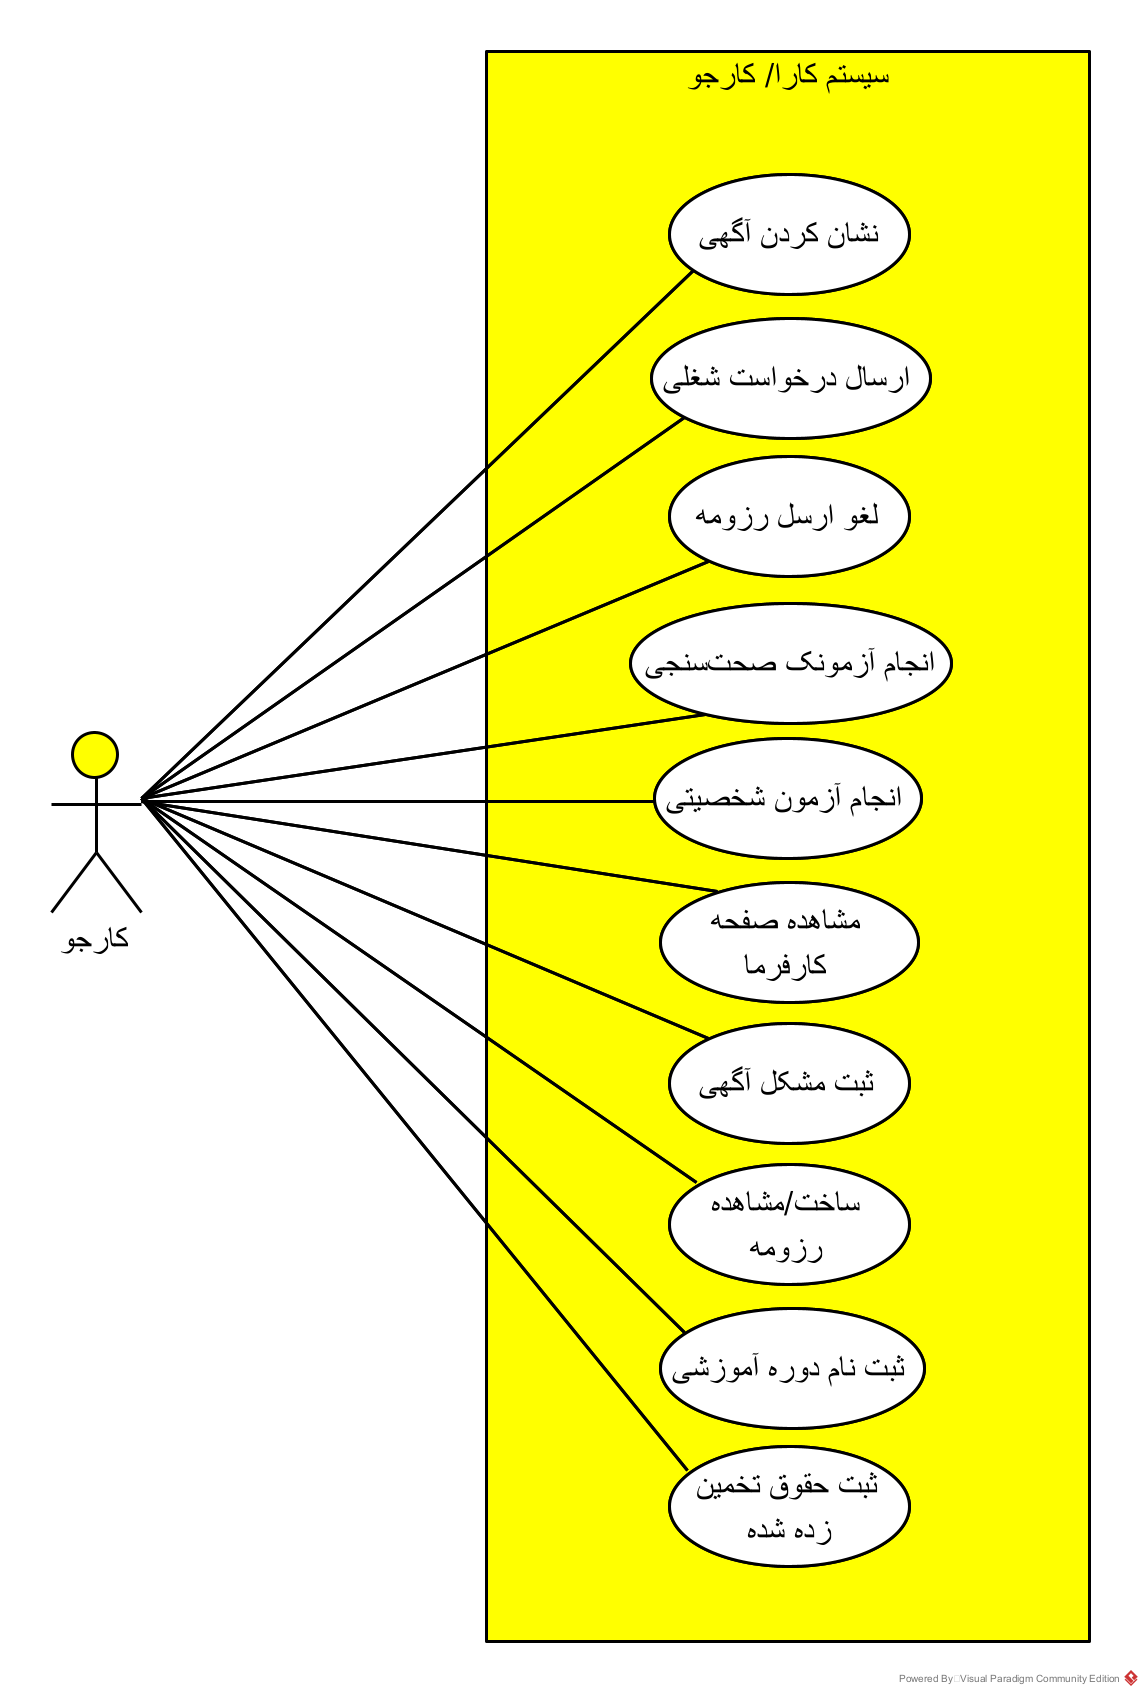
\includegraphics[width=0.7\linewidth]{files/UseCaseDiagram/UseCase_Employer}
		\caption{نمودار مورد کاربرد سامانه کارا برای کارفرما}
		\label{fig:usecaseemployer}
	\end{figure}

	\subsection{ماتریس ردیابی نیازمندی - مورد کاربرد}
در این بخش به جهت داشتن یک دید کلی از روابط بین مورد کاربردها و اولویت‌ها جدولی رسم خواهد شد که در آن مشخص می‌شود هر مورد کاربرد مربوط به کدام یک از نیازمندی‌ها است.
	\newpage
	\begin{longtable}{|c|c|c|c|c|c|c|c|c|c|c|c|}
		\caption{جدول ردیابی نیازمندی-مورد کاربرد، مورد کاربردهای 1 تا 10}
		\label{tab:req-uc-1-10}
		\endfirsthead
		\endhead
		\hline
		Req/UC      & R-Priority & U1       & U2       & U3       & U4       & U5       & U6       & U7       & U8       & U9       & U10      \\
		\hline
		R2          & 3          &           &           &           & \ding{51} &           &           &           &           &           &           \\
		\hline
		R5          & 2          &           &           &           &           & \ding{51} &           &           &           &           &           \\
		\hline
		R6          & 1          &           &           &           &           &           & \ding{51} &           &           &           &           \\
		\hline
		R9          & 3          &           &           &           &           &           &           & \ding{51} &           &           &           \\
		\hline
		R12         & 3          &           &           &           &           &           &           &           &           &           &           \\
		\hline
		R14         & 3          &           &           &           &           &           &           &           & \ding{51} &           &           \\
		\hline
		R15         & 1          & \ding{51} &           &           &           &           &           &           &           &           &           \\
		\hline
		R16         & 1          &           & \ding{51} &           &           &           &           &           &           &           &           \\
		\hline
		R17         & 1          &           &           & \ding{51} &           &           &           &           &           &           &           \\
		\hline
		R18         & 1          &           &           & \ding{51} &           &           &           &           &           &           &           \\
		\hline
		R19         & 3          &           &           &           &           &           &           &           &           & \ding{51} &           \\
		\hline
		R22         & 1          &           &           &           &           &           &           &           &           &           &           \\
		\hline
		R23         & 3          &           &           &           &           &           &           &           &           &           &           \\
		\hline
		R24         & 1          & \ding{51} &           &           &           &           &           &           &           &           &           \\
		\hline
		R25         & 1          & \ding{51} &           &           &           &           &           &           &           &           &           \\
		\hline
		R26         & 1          &           &           &           &           &           &           &           &           &           &           \\
		\hline
		R27         & 2          &           &           &           &           &           &           &           &           &           &           \\
		\hline
		R28         & 2          &           &           &           &           &           &           &           &           &           &           \\
		\hline
		R29         & 2          &           &           &           &           &           &           &           &           &           &           \\
		\hline
		R30         & 3          &           &           &           &           &           &           &           &           &           &           \\
		\hline
		R33         & 2          &           &           &           &           &           &           &           &           &           &           \\
		\hline
		R37         & 3          &           &           &           &           &           &           &           &           &           &           \\
		\hline
		R38         & 2          &           &           &           &           &           &           &           &           &           &           \\
		\hline
		R39         & 3          &           &           &           &           &           &           &           &           &           &           \\
		\hline
		R40         & 2          &           &           &           &           &           &           &           &           &           &           \\
		\hline
		R42         & 3          &           &           &           &           &           &           &           &           &           &           \\
		\hline
		R43         & 3          &           &           &           &           &           &           &           &           &           &           \\
		\hline
		R44         & 2          &           &           &           &           &           &           &           &           &           &           \\
		\hline
		R47         & 2          &           &           &           &           &           &           &           &           &           & \ding{51} \\
		\hline
		R50         & 3          &           &           &           &           &           &           &           &           &           &           \\
		\hline
		R52         & 1          &           &           &           &           &           &           &           &           &           &           \\
		\hline
		R53         & 2          &           &           &           &           &           &           &           &           &           &           \\
		\hline
		R55         & 1          &           &           &           &           &           &           &           &           &           &           \\
		\hline
		R61         & 3          &           &           &           &           &           &           &           &           &           &           \\
		\hline
		R63         & 3          &           &           &           &           &           &           &           &           &           &           \\
		\hline
		R66         & 1          &           &           &           &           &           &           &           &           &           &           \\
		\hline
		R67         & 1          &           &           &           &           &           &           &           &           &           &           \\
		\hline
		R68         & 1          &           &           &           &           &           &           &           &           &           &           \\
		\hline
		R69         & 3          &           &           &           &           &           &           &           &           &           &           \\
		\hline
		R71         & 2          &           &           &           &           &           &           &           &           &           &           \\
		\hline
		R72         & 1          &           &           &           &           &           &           &           &           &           &           \\
		\hline
		R73         & 2          &           &           &           &           &           &           &           &           &           &           \\
		\hline
		R74         & 3          &           &           &           &           &           &           &           &           &           &           \\
		\hline
		R76         & 2          &           &           &           &           &           &           &           &           &           &           \\
		\hline
		R78         & 2          &           &           &           &           &           &           &           &           &           &           \\
		\hline
		R79         & 3          &           &           &           &           &           &           &           &           &           &           \\
		\hline
		R83         & 3          &           &           &           &           &           &           &           &           &           &           \\
		\hline
		R84         & 3          &           &           &           &           &           &           &           &           &           &           \\
		\hline
		R85         & 2          &           &           &           &           &           &           &           &           &           &           \\
		\hline
		R86         & 2          &           &           &           &           &           &           &           &           &           &           \\
		\hline
		R94         & 3          &           &           &           &           &           &           &           &           &           &           \\
		\hline
		R96         & 3          &           &           &           &           &           &           &           &           &           &           \\
		\hline
		R97         & 3          &           &           &           &           &           &           &           &           &           &           \\
		\hline
		UC-Priority &            & 1         & 3         & 1         & 5         & 4         & 3         & 5         & 5         & 5         & 5         \\
		\hline
	\end{longtable}
	\newpage
	\begin{longtable}{|c|c|c|c|c|c|c|c|c|c|c|c|}
		\caption{جدول ردیابی نیازمندی-مورد کاربرد، مورد کاربردهای 11 تا 20}
		\label{tab:req-uc-11-20}
		\endfirsthead
		\endhead
		\hline
		Req/UC      & R-Priority & U11      & U12      & U13      & U14      & U15      & U16      & U17      & U18      & U19      & U20      \\
		\hline
		R2          & 3          &           &           &           &           &           &           &           &           &           &           \\
		\hline
		R5          & 2          &           &           &           &           &           &           &           &           &           &           \\
		\hline
		R6          & 1          &           &           &           &           &           &           &           &           &           &           \\
		\hline
		R9          & 3          &           &           &           &           &           &           &           &           &           &           \\
		\hline
		R12         & 3          &           &           &           &           &           &           &           &           &           &           \\
		\hline
		R14         & 3          &           &           &           &           &           &           &           &           &           &           \\
		\hline
		R15         & 1          &           &           &           &           &           &           &           &           &           &           \\
		\hline
		R16         & 1          &           &           &           &           &           &           &           &           &           &           \\
		\hline
		R17         & 1          &           &           &           &           &           &           &           &           &           &           \\
		\hline
		R18         & 1          &           &           &           &           &           &           &           &           &           &           \\
		\hline
		R19         & 3          &           &           &           &           &           &           &           &           &           &           \\
		\hline
		R22         & 1          &           &           &           & \ding{51} & \ding{51} &           &           &           &           &           \\
		\hline
		R23         & 3          &           &           &           &           &           & \ding{51} &           &           &           &           \\
		\hline
		R24         & 1          &           &           &           &           &           &           &           &           &           &           \\
		\hline
		R25         & 1          &           &           &           &           &           &           &           &           &           &           \\
		\hline
		R26         & 1          &           &           &           &           &           &           & \ding{51} &           &           &           \\
		\hline
		R27         & 2          &           & \ding{51} &           &           &           &           &           &           &           &           \\
		\hline
		R28         & 2          &           &           & \ding{51} &           &           &           &           &           &           &           \\
		\hline
		R29         & 2          &           &           &           &           &           &           &           & \ding{51} &           &           \\
		\hline
		R30         & 3          &           &           &           &           &           &           &           &           & \ding{51} &           \\
		\hline
		R33         & 2          &           &           &           &           &           & \ding{51} &           &           &           &           \\
		\hline
		R37         & 3          &           &           &           &           &           &           &           &           &           &           \\
		\hline
		R38         & 2          &           &           &           &           &           &           &           &           &           &           \\
		\hline
		R39         & 3          &           &           &           &           &           &           &           &           &           & \ding{51} \\
		\hline
		R40         & 2          &           &           &           &           &           & \ding{51} &           &           &           &           \\
		\hline
		R42         & 3          &           &           &           &           &           & \ding{51} &           &           &           &           \\
		\hline
		R43         & 3          &           &           &           &           &           &           &           &           &           &           \\
		\hline
		R44         & 2          &           &           &           &           &           &           &           &           &           &           \\
		\hline
		R47         & 2          & \ding{51} &           &           &           &           &           &           &           &           &           \\
		\hline
		R50         & 3          &           &           &           &           &           &           &           &           &           &           \\
		\hline
		R52         & 1          &           &           &           &           &           &           &           &           &           &           \\
		\hline
		R53         & 2          &           &           &           &           &           &           &           &           &           &           \\
		\hline
		R55         & 1          &           &           &           &           &           &           &           &           &           &           \\
		\hline
		R61         & 3          &           &           &           &           &           &           &           &           &           &           \\
		\hline
		R63         & 3          &           &           &           &           &           &           &           &           &           &           \\
		\hline
		R66         & 1          &           &           &           & \ding{51} &           &           &           &           &           &           \\
		\hline
		R67         & 1          &           &           &           & \ding{51} & \ding{51} &           & \ding{51} &           &           &           \\
		\hline
		R68         & 1          &           &           &           &           &           &           &           &           &           &           \\
		\hline
		R69         & 3          &           &           &           &           &           &           &           &           &           &           \\
		\hline
		R71         & 2          &           &           &           &           &           &           &           &           &           &           \\
		\hline
		R72         & 1          &           &           &           &           &           &           &           &           &           &           \\
		\hline
		R73         & 2          &           &           &           &           &           &           &           &           &           &           \\
		\hline
		R74         & 3          &           &           &           &           &           &           &           &           &           &           \\
		\hline
		R76         & 2          &           &           &           &           &           &           &           &           &           &           \\
		\hline
		R78         & 2          & \ding{51} &           &           &           &           &           &           &           &           &           \\
		\hline
		R79         & 3          &           &           &           &           &           &           &           &           &           &           \\
		\hline
		R83         & 3          &           &           &           &           &           &           &           &           &           &           \\
		\hline
		R84         & 3          &           &           &           &           &           &           &           &           &           &           \\
		\hline
		R85         & 2          &           &           &           &           &           &           &           &           &           &           \\
		\hline
		R86         & 2          &           &           &           &           &           &           &           &           &           &           \\
		\hline
		R94         & 3          &           &           &           &           &           &           &           &           &           &           \\
		\hline
		R96         & 3          &           &           &           &           &           &           &           &           &           &           \\
		\hline
		R97         & 3          &           &           &           &           &           &           &           &           &           &           \\
		\hline
		UC-Priority &            & 3         & 4         & 4         & 1         & 1         & 1         & 5         & 4         & 5         & 5         \\
		\hline
	\end{longtable}
	\newpage
	\begin{longtable}{|c|c|c|c|c|c|c|c|c|c|c|c|}
		\caption{جدول ردیابی نیازمندی-مورد کاربرد، مورد کاربردهای 21 تا 30}
		\label{tab:req-uc-21-30}
		\endfirsthead
		\endhead
		\hline
		Req/UC      & R-Priority & U21      & U22      & U23      & U24      & U25      & U26      & U27      & U28      & U29      & U30      \\
		\hline
		R2          & 3          &           &           &           &           &           &           &           &           &           &           \\
		\hline
		R5          & 2          &           &           &           &           &           &           &           &           &           &           \\
		\hline
		R6          & 1          &           &           &           &           &           &           &           &           &           &           \\
		\hline
		R9          & 3          &           &           &           &           &           &           &           &           &           &           \\
		\hline
		R12         & 3          &           &           &           &           &           &           &           &           &           &           \\
		\hline
		R14         & 3          &           &           &           &           &           &           &           &           &           &           \\
		\hline
		R15         & 1          &           &           &           &           &           &           &           &           &           &           \\
		\hline
		R16         & 1          &           &           &           &           &           &           &           &           &           &           \\
		\hline
		R17         & 1          &           &           &           &           &           &           &           &           &           &           \\
		\hline
		R18         & 1          &           &           &           &           &           &           &           &           &           &           \\
		\hline
		R19         & 3          &           &           &           &           &           &           &           &           &           &           \\
		\hline
		R22         & 1          &           &           &           &           &           &           &           &           &           &           \\
		\hline
		R23         & 3          &           &           &           &           &           &           &           &           &           &           \\
		\hline
		R24         & 1          &           &           &           &           &           &           &           &           &           &           \\
		\hline
		R25         & 1          &           &           &           &           &           &           &           &           &           &           \\
		\hline
		R26         & 1          &           &           &           &           &           &           &           &           &           &           \\
		\hline
		R27         & 2          &           &           &           &           &           &           &           &           &           &           \\
		\hline
		R28         & 2          &           &           &           &           &           &           &           &           &           &           \\
		\hline
		R29         & 2          &           &           &           &           &           &           &           &           &           &           \\
		\hline
		R30         & 3          &           &           &           &           &           &           &           &           &           &           \\
		\hline
		R33         & 2          &           &           &           &           &           &           &           &           &           &           \\
		\hline
		R37         & 3          &           &           &           &           &           &           &           &           &           &           \\
		\hline
		R38         & 2          &           &           &           &           &           &           &           &           &           &           \\
		\hline
		R39         & 3          &           &           &           &           &           &           &           &           &           &           \\
		\hline
		R40         & 2          &           &           &           &           &           &           &           &           &           &           \\
		\hline
		R42         & 3          &           &           &           &           &           &           &           &           &           &           \\
		\hline
		R43         & 3          & \ding{51} &           &           &           &           &           &           &           &           &           \\
		\hline
		R44         & 2          &           & \ding{51} &           &           &           &           &           &           &           &           \\
		\hline
		R47         & 2          &           &           &           &           &           &           &           &           &           &           \\
		\hline
		R50         & 3          &           &           & \ding{51} &           &           &           &           &           &           &           \\
		\hline
		R52         & 1          &           &           &           & \ding{51} &           &           &           &           &           &           \\
		\hline
		R53         & 2          &           &           &           &           & \ding{51} &           &           &           &           &           \\
		\hline
		R55         & 1          &           &           &           &           & \ding{51} &           &           &           &           &           \\
		\hline
		R61         & 3          &           &           &           &           &           & \ding{51} &           &           &           &           \\
		\hline
		R63         & 3          &           &           &           &           &           &           & \ding{51} &           &           &           \\
		\hline
		R66         & 1          &           &           &           &           &           &           &           &           &           &           \\
		\hline
		R67         & 1          &           &           &           &           &           &           &           &           &           &           \\
		\hline
		R68         & 1          &           &           &           &           &           &           &           & \ding{51} &           &           \\
		\hline
		R69         & 3          &           &           &           &           &           &           &           & \ding{51} &           &           \\
		\hline
		R71         & 2          &           &           &           &           &           &           &           &           &           & \ding{51} \\
		\hline
		R72         & 1          &           &           &           &           &           &           &           &           &           &           \\
		\hline
		R73         & 2          &           &           &           &           &           &           &           &           &           &           \\
		\hline
		R74         & 3          &           &           &           &           &           &           &           &           & \ding{51} &           \\
		\hline
		R76         & 2          &           &           &           &           &           &           &           &           &           &           \\
		\hline
		R78         & 2          &           &           &           &           &           &           &           &           &           &           \\
		\hline
		R79         & 3          &           &           &           &           &           &           &           &           &           &           \\
		\hline
		R83         & 3          &           &           &           &           &           &           &           &           &           &           \\
		\hline
		R84         & 3          &           &           &           &           &           &           &           & \ding{51} &           &           \\
		\hline
		R85         & 2          &           &           &           &           &           &           &           & \ding{51} &           &           \\
		\hline
		R86         & 2          &           &           &           &           &           &           &           &           &           &           \\
		\hline
		R94         & 3          &           &           &           &           &           &           &           &           &           &           \\
		\hline
		R96         & 3          &           &           &           &           &           &           &           &           &           &           \\
		\hline
		R97         & 3          &           &           &           &           &           &           &           &           &           &           \\
		\hline
		UC-Priority &            & 5         & 4         & 5         & 3         & 2         & 5         & 5         & 1         & 5         & 4         \\
		\hline
	\end{longtable}
	\newpage
	\begin{longtable}{|c|c|c|c|c|c|c|c|c|c|c|c|}
		\caption{جدول ردیابی نیازمندی-مورد کاربرد، مورد کاربردهای 31 تا 40}
		\label{tab:req-uc-31-40}
		\endfirsthead
		\endhead
		\hline
		Req/UC      & R-Priority & U31      & U32      & U33      & U34      & U35      & U36      & U37      & U38      & U39      & U40      \\
		\hline
		R2          & 3          &           &           &           &           &           &           &           &           &           &           \\
		\hline
		R5          & 2          &           &           &           &           &           &           &           &           &           &           \\
		\hline
		R6          & 1          &           &           &           &           &           &           &           &           &           &           \\
		\hline
		R9          & 3          &           &           &           &           &           &           &           &           &           &           \\
		\hline
		R12         & 3          &           &           &           &           &           &           &           &           & \ding{51} &           \\
		\hline
		R14         & 3          &           &           &           &           &           &           &           &           &           &           \\
		\hline
		R15         & 1          &           &           &           &           &           &           &           &           &           &           \\
		\hline
		R16         & 1          &           &           &           &           &           &           &           &           &           &           \\
		\hline
		R17         & 1          &           &           &           &           &           &           &           &           &           &           \\
		\hline
		R18         & 1          &           &           &           &           &           &           &           &           &           &           \\
		\hline
		R19         & 3          &           &           &           &           &           &           &           &           &           &           \\
		\hline
		R22         & 1          &           &           &           &           &           &           &           &           &           &           \\
		\hline
		R23         & 3          &           &           &           &           &           &           &           &           &           &           \\
		\hline
		R24         & 1          &           &           &           &           &           &           &           &           &           &           \\
		\hline
		R25         & 1          &           &           &           &           &           &           &           &           &           &           \\
		\hline
		R26         & 1          &           &           &           &           &           &           &           &           &           &           \\
		\hline
		R27         & 2          &           &           &           &           &           &           &           &           &           &           \\
		\hline
		R28         & 2          &           &           &           &           &           &           &           &           &           &           \\
		\hline
		R29         & 2          &           &           &           &           &           &           &           &           &           &           \\
		\hline
		R30         & 3          &           &           &           &           &           &           &           &           &           &           \\
		\hline
		R33         & 2          &           &           &           &           &           &           &           &           &           &           \\
		\hline
		R37         & 3          &           &           &           &           &           &           &           &           &           & \ding{51} \\
		\hline
		R38         & 2          &           &           &           &           &           &           &           &           &           & \ding{51} \\
		\hline
		R39         & 3          &           &           &           &           &           &           &           &           &           &           \\
		\hline
		R40         & 2          &           &           &           &           &           &           &           &           &           &           \\
		\hline
		R42         & 3          &           &           &           &           &           &           &           &           &           &           \\
		\hline
		R43         & 3          &           &           &           &           &           &           &           &           &           &           \\
		\hline
		R44         & 2          &           &           &           &           &           &           &           &           &           &           \\
		\hline
		R47         & 2          &           &           &           &           &           &           &           &           &           &           \\
		\hline
		R50         & 3          &           &           &           &           &           &           &           &           &           &           \\
		\hline
		R52         & 1          &           &           &           &           &           &           &           &           &           &           \\
		\hline
		R53         & 2          &           &           &           &           &           &           &           &           &           &           \\
		\hline
		R55         & 1          &           &           &           &           &           &           &           &           &           &           \\
		\hline
		R61         & 3          &           &           &           &           &           &           &           &           &           &           \\
		\hline
		R63         & 3          &           &           &           &           &           &           &           &           &           &           \\
		\hline
		R66         & 1          &           &           &           &           &           &           &           &           &           &           \\
		\hline
		R67         & 1          &           &           &           &           &           &           &           &           &           &           \\
		\hline
		R68         & 1          &           &           &           &           &           &           &           &           &           &           \\
		\hline
		R69         & 3          &           &           &           &           &           &           &           &           &           &           \\
		\hline
		R71         & 2          & \ding{51} &           &           &           &           &           &           &           &           &           \\
		\hline
		R72         & 1          & \ding{51} &           &           &           &           &           &           &           &           &           \\
		\hline
		R73         & 2          & \ding{51} &           &           &           &           &           &           &           &           &           \\
		\hline
		R74         & 3          & \ding{51} &           &           &           &           &           &           &           &           &           \\
		\hline
		R76         & 2          &           & \ding{51} &           &           &           &           &           &           &           &           \\
		\hline
		R78         & 2          &           &           &           &           &           &           &           &           &           &           \\
		\hline
		R79         & 3          &           &           & \ding{51} &           &           &           &           &           &           &           \\
		\hline
		R83         & 3          &           &           &           & \ding{51} &           &           &           &           &           &           \\
		\hline
		R84         & 3          &           &           &           &           &           &           &           &           &           &           \\
		\hline
		R85         & 2          &           &           &           &           &           &           &           &           &           &           \\
		\hline
		R86         & 2          &           &           &           &           & \ding{51} &           &           &           &           &           \\
		\hline
		R94         & 3          &           &           &           &           &           & \ding{51} &           &           &           &           \\
		\hline
		R96         & 3          &           &           &           &           &           &           & \ding{51} &           &           &           \\
		\hline
		R97         & 3          &           &           &           &           &           &           &           & \ding{51} &           &           \\
		\hline
		UC-Priority &            & 1         & 4         & 5         & 5         & 4         & 5         & 5         & 5         & 5         & 4         \\
		\hline
	\end{longtable}
	\newpage

	\subsection{تخصیص مورد کاربردها به تکرارها}
	در گام‌های قبل مورد کاربردها شناسایی و نمودارهای آنها ترسیم شدند. سپس اولویت هر کدام از مورد کاربردها برای توسعه به دست آمد.\\
	حال باید یک زمان‌بندی برای توسعه و تحویل مورد کاربردها تولید شود که در آن برنامه‌ریزی شود که در هر تکرار چه مورد کاربردهایی توسعه یابند و به تحویل مشتری داده شوند.
	این زمان‌بندی به سه عامل بستگی دارد:
	\begin{itemize}
		\item اولویت مورد کاربردها
		این اولویت‌ها خود بر اساس اولویت نیازمندی‌ها بدست آمده اند؛ هر چه میزان اولویت کمتر باشد به این معنی است که مورد کاربرد مورد نظر باید زودتر توسعه و تحویل داده شود. در این جدول اولویت‌ها بر اساس تکرارهای موجود از بین یک تا پنج شماره گذاری شده‌اند.
		\item وابستگی مورد کاربردها به یکدیگر
		به این صورت که اگر مورد کاربرد "ب" به مورد کاربرد "الف" وابسته باشد، بدون وجود مورد کاربرد "الف"، کاربر به مورد کاربرد "ب" دسترسی نخواهد داشت.
		\item توانایی تیم توسعه دهنده
		از آن‌جایی که یک تیم هفت نفره بر روی این پروژه کار می‌کنند، میزان تلاش هفت نفر در هفته در نظر گرفته شده و از سمت دیگر به علت اینکه هر تکرار به صورت یک بازه‌ پنج هفته‌ای در نظر گرفته شده، حداکثر میزان تلاش در تکرارها، 35 نفر در هفته می‌باشد. بر این اساس به هر یک از مورد کاربردها یک میزان تلاش تخمینی نسبت داده شده است.
	\end{itemize}

	\begin{longtable}{|c|ccc|l|l|l|}
		\caption{جدول تخصیص مورد کاربردها به تکرارها}
		\label{tab:uc-to-rep}
		\endfirsthead
		\endhead
		\hline
		\textbf{مورد کاربرد} & \multicolumn{1}{c|}{\textbf{اولویت}} & \multicolumn{1}{c|}{\textbf{\begin{tabular}[c]{@{}c@{}}میزان تلاش\\ (نفر- هفته)\end{tabular}}} & \textbf{وابسته به} & \multicolumn{1}{c|}{\textbf{\begin{tabular}[c]{@{}c@{}}تکرار اول\\ (پنج هفته)\end{tabular}}} & \multicolumn{1}{c|}{\textbf{\begin{tabular}[c]{@{}c@{}}تکرار دوم\\ (پنج هفته)\end{tabular}}} & \multicolumn{1}{c|}{\textbf{\begin{tabular}[c]{@{}c@{}}تکرار سوم\\ (پنج هفته)\end{tabular}}} \\ \hline
		UC1                  & \multicolumn{1}{c|}{1}               & \multicolumn{1}{c|}{2}                                                                         & None               & \multicolumn{1}{c|}{2}                                                                     &                                                                                               &                                                                                            \\ \hline
		UC2                  & \multicolumn{1}{c|}{3}               & \multicolumn{1}{c|}{2}                                                                         & UC1                & \multicolumn{1}{c|}{2}                                                                     &                                                                                               &                                                                                            \\ \hline
		UC3                  & \multicolumn{1}{c|}{1}               & \multicolumn{1}{c|}{1}                                                                         & UC5                & \multicolumn{1}{c|}{1}                                                                     &                                                                                               &                                                                                            \\ \hline
		UC4                  & \multicolumn{1}{c|}{5}               & \multicolumn{1}{c|}{3}                                                                         & UC1                &                                                                                            &                                                                                               & \multicolumn{1}{c|}{3}                                                                     \\ \hline
		UC5                  & \multicolumn{1}{c|}{4}               & \multicolumn{1}{c|}{1}                                                                         & None               & \multicolumn{1}{c|}{1}                                                                     &                                                                                               &                                                                                            \\ \hline
		UC6                  & \multicolumn{1}{c|}{3}               & \multicolumn{1}{c|}{1}                                                                         & None               & \multicolumn{1}{c|}{1}                                                                     &                                                                                               &                                                                                            \\ \hline
		UC7                  & \multicolumn{1}{c|}{5}               & \multicolumn{1}{c|}{1}                                                                         & UC1                &                                                                                            &                                                                                               & \multicolumn{1}{c|}{1}                                                                     \\ \hline
		UC8                  & \multicolumn{1}{c|}{5}               & \multicolumn{1}{c|}{2}                                                                         & UC1                &                                                                                            &                                                                                               & \multicolumn{1}{c|}{2}                                                                     \\ \hline
		UC9                  & \multicolumn{1}{c|}{5}               & \multicolumn{1}{c|}{5}                                                                         & UC27               &                                                                                            & \multicolumn{1}{c|}{5}                                                                        &                                                                                            \\ \hline
		UC10                 & \multicolumn{1}{c|}{5}               & \multicolumn{1}{c|}{4}                                                                         & UC11               & \multicolumn{1}{c|}{4}                                                                     &                                                                                               &                                                                                            \\ \hline
		UC11                 & \multicolumn{1}{c|}{3}               & \multicolumn{1}{c|}{4}                                                                         & None               & \multicolumn{1}{c|}{4}                                                                     &                                                                                               &                                                                                            \\ \hline
		UC12                 & \multicolumn{1}{c|}{4}               & \multicolumn{1}{c|}{2}                                                                         & UC28               &                                                                                            & \multicolumn{1}{c|}{2}                                                                        &                                                                                            \\ \hline
		UC13                 & \multicolumn{1}{c|}{4}               & \multicolumn{1}{c|}{2}                                                                         & UC28               &                                                                                            & \multicolumn{1}{c|}{2}                                                                        &                                                                                            \\ \hline
		UC14                 & \multicolumn{1}{c|}{1}               & \multicolumn{1}{c|}{2}                                                                         & UC6                & \multicolumn{1}{c|}{2}                                                                     &                                                                                               &                                                                                            \\ \hline
		UC15                 & \multicolumn{1}{c|}{1}               & \multicolumn{1}{c|}{2}                                                                         & UC6                & \multicolumn{1}{c|}{2}                                                                     &                                                                                               &                                                                                            \\ \hline
		UC16                 & \multicolumn{1}{c|}{1}               & \multicolumn{1}{c|}{3}                                                                         & UC28               & \multicolumn{1}{c|}{3}                                                                     &                                                                                               &                                                                                            \\ \hline
		UC17                 & \multicolumn{1}{c|}{5}               & \multicolumn{1}{c|}{2}                                                                         & UC16               &                                                                                            &                                                                                               & \multicolumn{1}{c|}{2}                                                                     \\ \hline
		UC18                 & \multicolumn{1}{c|}{4}               & \multicolumn{1}{c|}{3}                                                                         & UC16, UC24         &                                                                                            & \multicolumn{1}{c|}{3}                                                                        &                                                                                            \\ \hline
		UC19                 & \multicolumn{1}{c|}{5}               & \multicolumn{1}{c|}{1}                                                                         & UC18               &                                                                                            &                                                                                               & \multicolumn{1}{c|}{1}                                                                     \\ \hline
		UC20                 & \multicolumn{1}{c|}{5}               & \multicolumn{1}{c|}{4}                                                                         & UC15               &                                                                                            &                                                                                               & \multicolumn{1}{c|}{4}                                                                     \\ \hline
		UC21                 & \multicolumn{1}{c|}{5}               & \multicolumn{1}{c|}{2}                                                                         & UC16               &                                                                                            &                                                                                               & \multicolumn{1}{c|}{2}                                                                     \\ \hline
		UC22                 & \multicolumn{1}{c|}{4}               & \multicolumn{1}{c|}{1}                                                                         & UC16               &                                                                                            & \multicolumn{1}{c|}{1}                                                                        &                                                                                            \\ \hline
		UC23                 & \multicolumn{1}{c|}{5}               & \multicolumn{1}{c|}{2}                                                                         & None               &                                                                                            &                                                                                               & \multicolumn{1}{c|}{2}                                                                     \\ \hline
		UC24                 & \multicolumn{1}{c|}{3}               & \multicolumn{1}{c|}{4}                                                                         & UC15               & \multicolumn{1}{c|}{4}                                                                     &                                                                                               &                                                                                            \\ \hline
		UC25                 & \multicolumn{1}{c|}{2}               & \multicolumn{1}{c|}{1}                                                                         & UC24               & \multicolumn{1}{c|}{1}                                                                     &                                                                                               &                                                                                            \\ \hline
		UC26                 & \multicolumn{1}{c|}{5}               & \multicolumn{1}{c|}{2}                                                                         & UC4                &                                                                                            &                                                                                               & \multicolumn{1}{c|}{2}                                                                     \\ \hline
		UC27                 & \multicolumn{1}{c|}{5}               & \multicolumn{1}{c|}{2}                                                                         & UC1                &                                                                                            & \multicolumn{1}{c|}{2}                                                                        &                                                                                            \\ \hline
		UC28                 & \multicolumn{1}{c|}{1}               & \multicolumn{1}{c|}{4}                                                                         & None               & \multicolumn{1}{c|}{4}                                                                     &                                                                                               &                                                                                            \\ \hline
		UC29                 & \multicolumn{1}{c|}{5}               & \multicolumn{1}{c|}{3}                                                                         & UC28               & \multicolumn{1}{c|}{3}                                                                     &                                                                                               &                                                                                            \\ \hline
		UC30                 & \multicolumn{1}{c|}{4}               & \multicolumn{1}{c|}{2}                                                                         & UC28               &                                                                                            & \multicolumn{1}{c|}{2}                                                                        &                                                                                            \\ \hline
		UC31                 & \multicolumn{1}{c|}{1}               & \multicolumn{1}{c|}{1}                                                                         & UC28               &                                                                                            & \multicolumn{1}{c|}{1}                                                                        &                                                                                            \\ \hline
		UC32                 & \multicolumn{1}{c|}{4}               & \multicolumn{1}{c|}{1}                                                                         & UC18               &                                                                                            & \multicolumn{1}{c|}{1}                                                                        &                                                                                            \\ \hline
		UC33                 & \multicolumn{1}{c|}{5}               & \multicolumn{1}{c|}{4}                                                                         & UC24               &                                                                                            & \multicolumn{1}{c|}{4}                                                                        &                                                                                            \\ \hline
		UC34                 & \multicolumn{1}{c|}{5}               & \multicolumn{1}{c|}{3}                                                                         & UC32               &                                                                                            &                                                                                               & \multicolumn{1}{c|}{3}                                                                     \\ \hline
		UC35                 & \multicolumn{1}{c|}{4}               & \multicolumn{1}{c|}{1}                                                                         & UC32               &                                                                                            & \multicolumn{1}{c|}{1}                                                                        &                                                                                            \\ \hline
		UC36                 & \multicolumn{1}{c|}{5}               & \multicolumn{1}{c|}{1}                                                                         & UC37               &                                                                                            &                                                                                               & \multicolumn{1}{c|}{1}                                                                     \\ \hline
		UC37                 & \multicolumn{1}{c|}{5}               & \multicolumn{1}{c|}{4}                                                                         & None               &                                                                                            &                                                                                               & \multicolumn{1}{c|}{4}                                                                     \\ \hline
		UC38                 & \multicolumn{1}{c|}{5}               & \multicolumn{1}{c|}{4}                                                                         & UC28               &                                                                                            &                                                                                               & \multicolumn{1}{c|}{4}                                                                     \\ \hline
		UC39                 & \multicolumn{1}{c|}{5}               & \multicolumn{1}{c|}{2}                                                                         & None               &                                                                                            & \multicolumn{1}{c|}{2}                                                                        &                                                                                            \\ \hline
		UC40                 & \multicolumn{1}{c|}{4}               & \multicolumn{1}{c|}{3}                                                                         & UC28               &                                                                                            & \multicolumn{1}{c|}{3}                                                                        &                                                                                            \\ \hline
		\textbf{جمع تلاش}    & \multicolumn{3}{l|}{94}                                                                                                                                    & 34                                                                                         & 29                                                                                            & 31                                                                                         \\ \hline
	\end{longtable}

	\subsection{مدل‌سازی تعامل کنشگر سیستم}
	بعد از مشخص شدن مورد کاربردها، برای برخی از آنها چگونگی تعامل کنشگر با سیستم را مشخص کرده‌ایم. مورد کاربردهایی برای این کار انتخاب شده‌اند که جزئیات آنها از اهمیت بالاتری برخوردار هستند.
	برای این کار از یک جدول دو ستونی استفاده شده است که ستون راست ورودی کنشگرهای مورد نظر و ستون سمت چپ پاسخ‌های سیستم را مشخص می‌کند.

	\begin{center}
		\begin{table}[H]
			\caption{جدول مورد کاربرد گسترده 9}
			\label{tab:ext-uc9}
			\begin{tabular}{|rr|}
				\hline
				\rowcolor{Gainsboro!60}
				\multicolumn{2}{|r|}{\textbf{:UC9 مشاهده حقوق تخمین زده شده از ماشین حساب حقوق}}                                                                                                                                                                           \\ \hline
				\multicolumn{2}{|r|}{\textbf{پیش شرط: -}}                                                                                                                                                                                                                                          \\ \hline
				\multicolumn{1}{|c|}{\textbf{کنشگر: کاربر بازدیدکننده}}                                                                                            & \multicolumn{1}{c|}{\textbf{سیستم:سامانه کارا}}                                                                               \\ \hline
				\multicolumn{1}{|c|}{\textbf{}}                                                                                                                    & ۰-  سیستم صفحه اصلی را نشان می‌دهد.                                                                                           \\ \hline
				\multicolumn{1}{|r|}{\begin{tabular}[c]{@{}r@{}}۱- TUCBW کاربر بازدیدکننده در صفحه  روی پیوند \\ «ماشین حساب حقوق» کلیک می‌کند.\end{tabular}}      & \begin{tabular}[c]{@{}r@{}}۲- سیستم دو گزینه «ثبت حقوق دریافتی» \\ و «تخمین حقوق» را نمایش می‌دهد.\end{tabular}               \\ \hline
				\multicolumn{1}{|r|}{\begin{tabular}[c]{@{}r@{}}۳- کاربر بازدیدکننده روی گزینه «تخمین حقوق»\\  کلیک می‌کند.\end{tabular}}                          & \begin{tabular}[c]{@{}r@{}}۴- سیستم فرمی شامل اطلاعات عنوان شغلی، \\ سطح ارشدیت، سابقه کاری و … را نمایش می‌دهد.\end{tabular} \\ \hline
				\multicolumn{1}{|r|}{\begin{tabular}[c]{@{}r@{}}۵- کاربر بازدیدکننده اطلاعات خود را وارد می‌کند\\  سپس روی دکمه «تخمین» کلیک می‌کند.\end{tabular}} & \begin{tabular}[c]{@{}r@{}}۶- سیستم براساس اطلاعات موجود یک \\ حقوق تخمین زده شده را نمایش می‌دهد.\end{tabular}               \\ \hline
				\multicolumn{1}{|r|}{\begin{tabular}[c]{@{}r@{}}۷- TUCEW کاربر بازدیدکننده حقوق\\  تخمین زده شده را مشاهده می‌کند.\end{tabular}}                   & \multicolumn{1}{l|}{}                                                                                                         \\ \hline

			\end{tabular}
		\end{table}

		\begin{table}[H]
			\caption{جدول مورد کاربرد گسترده 11}
			\label{tab:ext-uc11}
			\begin{tabular}{|rr|}
				\hline
				\rowcolor{Gainsboro!60}
				\multicolumn{2}{|r|}{\textbf{:UC11 ارسال پیام خصوصی}}                                                                                                                                                                                                                                                                                                                                        \\ \hline
				\multicolumn{2}{|r|}{\textbf{پیش شرط: کاربر باید وارد حساب کاربری خود شده باشد.}}                                                                                                                                                                                                                                                                                                                                    \\ \hline
				\multicolumn{1}{|c|}{\textbf{کنشگر:کاربر}}                                                                                                                                                                                                                    & \multicolumn{1}{c|}{\textbf{سیستم:سامانه کارا}}                                                                                                      \\ \hline
				\multicolumn{1}{|l|}{\textbf{}}                                                                                                                                                                                                                               & ۰- سیستم صفحه اصلی را نمایش می‌دهد.                                                                                                                  \\ \hline
				\multicolumn{1}{|r|}{\begin{tabular}[c]{@{}r@{}}۱- TUCBW کاربر روی پیوند "پیام خصوصی"\\  در صفحه اصلی کلیک می‌کند.\end{tabular}}                                                                                                                              & ۲- سیستم صفحه پیام‌رسان را نمایش می‌دهد.                                                                                                             \\ \hline
				\multicolumn{1}{|r|}{\begin{tabular}[c]{@{}r@{}}۳-\\ الف) اگر این اولین پیام خصوصی به کاربر مورد نظر \\ است، کاربر ایمیل شخص مورد نظر را وارد می‌کند.\\  ب) درغیر این‌صورت، کاربر مورد نظر را از\\ لیست گفتگوها برای ارسال پیام انتخاب می‌کند.\end{tabular}} & \begin{tabular}[c]{@{}r@{}}۴- در صورت موجود بودن شخص، صفحه‌ی گفتگو \\ شخص مورد نظر به همراه فیلد شرح پیام و پیوست \\ نمایش داده می‌شود.\end{tabular} \\ \hline
				\multicolumn{1}{|r|}{\begin{tabular}[c]{@{}r@{}}۵- کاربر صفحه گفتگو را مشاهده می‌کند و \\ متن پیام خود را وارد می‌کند. در نهایت روی دکمه \\ "ارسال" کلیک می‌کند.\end{tabular}}                                                                                & \begin{tabular}[c]{@{}r@{}}۶- سیستم پیامی متناسب با نتیجه\\  ارسال پیام نمایش می‌دهد.\end{tabular}                                                   \\ \hline
				\multicolumn{1}{|r|}{\begin{tabular}[c]{@{}r@{}}۷- TUCEW کاربر نتیجه ارسال پیام خصوصی \\ خود را مشاهده می‌کند.\end{tabular}}                                                                                                                                  & \multicolumn{1}{l|}{}                                                                                                                                \\ \hline

			\end{tabular}
		\end{table}

		\begin{table}[H]
			\caption{جدول مورد کاربرد گسترده 13}
			\label{tab:ext-uc13}
			\begin{tabular}{|rr|}
				\hline
				\rowcolor{Gainsboro!60}
				\multicolumn{2}{|r|}{\textbf{:UC13 جستجوی پیشرفته}}                                                                                                                                                                                                                                           \\ \hline
				\multicolumn{2}{|r|}{\textbf{پیش شرط: -}}                                                                                                                                                                                                                                                                             \\ \hline
				\multicolumn{1}{|c|}{\textbf{کنشگر: کاربر}}                                                                                           & \multicolumn{1}{c|}{\textbf{سیستم: سامانه کارا}}                                                                                                                              \\ \hline
				\multicolumn{1}{|l|}{\textbf{}}                                                                                                       & ۰- سیستم صفحه اصلی را نمایش می‌دهد.                                                                                                                                           \\ \hline
				\multicolumn{1}{|r|}{\begin{tabular}[c]{@{}r@{}}۱- TUCBW کاربر روی پیوند «جستجوی \\ پیشرفته» در صفحه اصلی کلیک می‌کند.\end{tabular}}  & \begin{tabular}[c]{@{}r@{}}۲- سیستم صفحه جستجوی پیشرفته و گزینه‌های\\  پالایه جستجوی پیشرفته مانند گروه شغلی،\\  شهر، نوع همکاری، سبک تعامل و … را نمایش می‌دهد.\end{tabular} \\ \hline
				\multicolumn{1}{|r|}{\begin{tabular}[c]{@{}r@{}}۳- کاربر اطلاعات مورد نظر خود را \\ در صفحه جستجوی پیشرفته وارد می‌کند.\end{tabular}} & \begin{tabular}[c]{@{}r@{}}۴- سیستم نتیجه‌ی جستجوی کاربر\\  را در قالب یک لیست نمایش می‌دهد.\end{tabular}                                                                     \\ \hline
				\multicolumn{1}{|r|}{\begin{tabular}[c]{@{}r@{}}۵- TUCEW کاربر نتیجه جستجوی خود\\  را مشاهده می‌کند.\end{tabular}}                    & \multicolumn{1}{l|}{}                                                                                                                                                         \\ \hline

			\end{tabular}
		\end{table}

		\begin{table}[H]
			\caption{جدول مورد کاربرد گسترده 18}
			\label{tab:ext-uc18}
			\begin{tabular}{|rr|}
				\hline
				\rowcolor{Gainsboro!60}
				\multicolumn{2}{|r|}{\textbf{:UC18 ارسال درخواست شغلی}}                                                                                                                                                                                                                                                                                                                                                    \\ \hline
				\multicolumn{2}{|r|}{\textbf{پیش شرط: کارجو باید وارد حساب کاربری خود شده باشد و رزومه ساخته باشد.}}                                                                                                                                                                                                                                                                                                                               \\ \hline
				\multicolumn{1}{|c|}{\textbf{کنشگر: کارجو}}                                                                                                                                        & \multicolumn{1}{c|}{\textbf{سیستم:سامانه کارا}}                                                                                                                                                                                               \\ \hline
				\multicolumn{1}{|l|}{\textbf{}}                                                                                                                                                    & ۰- سیستم صفحه آگهی را به کارجو نمایش می‌دهد.                                                                                                                                                                                                  \\ \hline
				\multicolumn{1}{|r|}{\begin{tabular}[c]{@{}r@{}}۱- TUCBW کارجو روی گزینه «ارسال \\ درخواست شغلی» در صفحه آگهی کلیک می‌کند.\end{tabular}}                                           & \begin{tabular}[c]{@{}r@{}}۲- سیستم صفحه تایید اطلاعات و پیش شرط‌های\\  لازم مانند تست شخصیتی و فرم پرسشنامه\\  برای ارسال درخواست را به کارجو نمایش می‌دهد.\end{tabular}                                                                     \\ \hline
				\multicolumn{1}{|r|}{\begin{tabular}[c]{@{}r@{}}3- در صورت وجود فرم پرسشنامه، کاربر\\  آن را تکمیل می‌کند.در نهایت روی گزینه \\ "تایید و ارسال درخواست" کلیک می‌کند.\end{tabular}} & \begin{tabular}[c]{@{}r@{}}4- \\ الف) در صورتی که درصد تطابق رزومه و آگهی\\  بالاتر از ۵۰ درصد بود سیستم پیام \\ "ارسال درخواست شغلی با موفقیت انجام شد." \\  را نمایش می‌دهد.\\ ب) درغیر این‌صورت سیستم پیام خطا نمایش می‌دهد.\end{tabular} \\ \hline
				\multicolumn{1}{|r|}{\begin{tabular}[c]{@{}r@{}}5- TUCEW کارجو نتیجه ارسال درخواست\\  شغلی خود را در قالب پیام مناسب \\ مشاهده می‌کند.\end{tabular}}                            & \multicolumn{1}{l|}{}                                                                                                                                                                                                                         \\ \hline

			\end{tabular}
		\end{table}

		\begin{table}[ht]
			\caption{جدول مورد کاربرد گسترده 21}
			\label{tab:ext-uc21}
			\centering

			\begin{tabular}{|rr|}
				\hline
				\rowcolor{Gainsboro!60}
				\multicolumn{2}{|r|}{\textbf{:UC21 ثبت مشکل آگهی}}                                                                                                                                                                        \\ \hline
				\multicolumn{2}{|r|}{\textbf{پیش شرط: -  کارجو باید وارد حساب کاربری خود شده باشد.}}                                                                                                                                                              \\ \hline
				\multicolumn{1}{|c|}{\textbf{کنشگر: کارجو}}                                                                                   & \multicolumn{1}{c|}{\textbf{سیستم:سامانه کارا}}                                                                   \\ \hline
				\multicolumn{1}{|l|}{\textbf{}}                                                                                               & \begin{tabular}[c]{@{}r@{}}۰- سیستم صفحه آگهی شغلی را\\  نمایش می‌دهد.\end{tabular}                               \\ \hline
				\multicolumn{1}{|r|}{\begin{tabular}[c]{@{}r@{}}۱- TUCBW کارجو بر روی «ثبت مشکل»\\  در صفحه آگهی کلیک می‌کند.\end{tabular}}   & \begin{tabular}[c]{@{}r@{}}۲- سیستم یک فرم ثبت مشکل که شامل عنوان\\  و شرح مشکل است را نمایش می‌دهد.\end{tabular} \\ \hline
				\multicolumn{1}{|r|}{\begin{tabular}[c]{@{}r@{}}۳- کارجو اطلاعات را وارد کرده\\  و روی گزینه "ثبت" کلیک می‌کند.\end{tabular}} & \begin{tabular}[c]{@{}r@{}}۴- سیستم پیغام «مشکل با موفقیت\\  ثبت شد» را نمایش می‌دهد.\end{tabular}                \\ \hline
				\multicolumn{1}{|r|}{\begin{tabular}[c]{@{}r@{}}۵- TUCEW کارجو پیغام مناسب\\  را مشاهده می‌کند.\end{tabular}}                 & \multicolumn{1}{l|}{}                                                                                             \\ \hline

			\end{tabular}
		\end{table}

		\begin{table}[H]
			\caption{جدول مورد کاربرد گسترده 24}
			\label{tab:ext-uc24}
			\begin{tabular}{|rr|}
				\hline
				\rowcolor{Gainsboro!60}
				\multicolumn{2}{|r|}{\textbf{:UC24 ساخت رزومه}}                                                                                                                                                                                                                                                                                           \\ \hline
				\multicolumn{2}{|r|}{\textbf{پیش‌ شرط: کارجو باید اطلاعات کاربری خود را تکمیل کرده باشد.}}                                                                                                                                                                                                                                                                        \\ \hline
				\multicolumn{1}{|c|}{\textbf{کنشگر: کارجو}}                                                                                                             & \multicolumn{1}{c|}{\textbf{سیستم: سامانه کارا}}                                                                                                                                                        \\ \hline
				\multicolumn{1}{|l|}{\textbf{}}                                                                                                                         & ۰- سیستم صفحه کاربری کارجو را نمایش می‌دهد.                                                                                                                                                             \\ \hline
				\multicolumn{1}{|r|}{\begin{tabular}[c]{@{}r@{}}۱- TUCBW کارجو بر روی گزینه "ساخت رزومه" \\ در صفحه کاربری خود کلیک می‌کند.\end{tabular}}               & \begin{tabular}[c]{@{}r@{}}۲- سیستم صفحه ساخت رزومه که شامل فرمی \\ از اطلاعات مانند درباره من، اطلاعات تحصیلی، \\ سوابق شغلی، مهارت‌ها و … را به دو\\  زبان انگلیسی و فارسی نمایش می‌دهد.\end{tabular} \\ \hline
				\multicolumn{1}{|r|}{\begin{tabular}[c]{@{}r@{}}۳- کاربر اطلاعات خود را به فارسی یا \\ انگلیسی وارد می‌کند و روی دکمه\\  ثبت کلیک می‌کند.\end{tabular}} & \begin{tabular}[c]{@{}r@{}}۴- سیستم نتیجه ساخت رزومه \\ را به کاربر نمایش می‌دهد.\end{tabular}                                                                                                          \\ \hline
				\multicolumn{1}{|r|}{\begin{tabular}[c]{@{}r@{}}۵- TUCEW کارجو نتیجه ساخت رزومه \\ خود را مشاهده می‌کند.\end{tabular}}                                  & \multicolumn{1}{l|}{}                                                                                                                                                                                   \\ \hline

			\end{tabular}
		\end{table}

		\begin{table}[H]
			\caption{جدول مورد کاربرد گسترده 28}
			\label{tab:ext-uc28}
			\begin{tabular}{|rr|}
				\hline
				\rowcolor{Gainsboro!60}
				\multicolumn{2}{|r|}{\textbf{:UC28 ثبت آگهی}}                                                                                                                                                                                                                                                 \\ \hline
				\multicolumn{2}{|r|}{\textbf{پیش شرط: کارفرما باید وارد حساب کاربری خود شده باشد.}}                                                                                                                                                                                                                                   \\ \hline
				\multicolumn{1}{|c|}{\textbf{کنشگر: کارفرما}}                                                                                          & \multicolumn{1}{c|}{\textbf{سیستم: سامانه کارا}}                                                                                                                             \\ \hline
				\multicolumn{1}{|l|}{\textbf{}}                                                                                                        & ۰- سیستم صفحه کاربری کارفرما را نمایش می‌دهد.                                                                                                                                \\ \hline
				\multicolumn{1}{|r|}{\begin{tabular}[c]{@{}r@{}}۱- TUCBW کارفرما روی گزینه «ثبت آگهی» در\\  صفحه کاربری خود کلیک می‌کند.\end{tabular}} & \begin{tabular}[c]{@{}r@{}}۲- سیستم صفحه‌ی ساخت آگهی را که شامل فرمی \\ از اطلاعاتی مانند عنوان شغلی، نوع همکاری، \\ بازه حقوق، سطح ارشدیت و … را نمایش می‌دهد.\end{tabular} \\ \hline
				\multicolumn{1}{|r|}{\begin{tabular}[c]{@{}r@{}}۳- کاربر اطلاعات خود را وارد می‌کند \\ و سپس روی دکمه «ثبت» کلیک می‌کند.\end{tabular}} & \begin{tabular}[c]{@{}r@{}}۴- سیستم در صورت معتبر بودن اطلاعات، \\ آگهی را می‌سازد و نتیجه را به کاربر نمایش می‌دهد.\end{tabular}                                            \\ \hline
				\multicolumn{1}{|r|}{\begin{tabular}[c]{@{}r@{}}۵- TUCEW کارفرما نتیجه ساخت آگهی خود\\  را مشاهده می‌کند.\end{tabular}}                & \multicolumn{1}{l|}{}                                                                                                                                                        \\ \hline

			\end{tabular}
		\end{table}
	\end{center}
	\newpage

\end{document}